% \documentclass[mat2, tisk]{fmfdelo}
% \documentclass[fin2, tisk]{fmfdelo}
% \documentclass[isrm2, tisk]{fmfdelo}
\documentclass[ped, tisk]{fmfdelo}
% Če pobrišete možnost tisk, bodo povezave obarvane,
% na začetku pa ne bo praznih strani po naslovu, …

%%%%%%%%%%%%%%%%%%%%%%%%%%%%%%%%%%%%%%%%%%%%%%%%%%%%%%%%%%%%%%%%%%%%%%%%%%%%%%%
% METAPODATKI
%%%%%%%%%%%%%%%%%%%%%%%%%%%%%%%%%%%%%%%%%%%%%%%%%%%%%%%%%%%%%%%%%%%%%%%%%%%%%%%

% - vaše ime
\avtor{Terezija Krečič}

% - naslov dela v slovenščini
\naslov{Origami konstrukcije in reševanje enačb s prepogibanjem papirja}

% - naslov dela v angleščini
\title{Origami constructions and solving equations by paper-folding}

% - ime mentorja/mentorice s polnim nazivom:
%   - doc.~dr.~Ime Priimek
%   - izr.~prof.~dr.~Ime Priimek
%   - prof.~dr.~Ime Priimek
%   za druge variante uporabite ustrezne ukaze
\mentor{prof.~dr.~Aleš Vavpetič}
% \somentor{...}
% \mentorica{...}
% \somentorica{...}
% \mentorja{...}{...}
% \somentorja{...}{...}
% \mentorici{...}{...}
% \somentorici{...}{...}

% - leto magisterija
\letnica{2025}

% - povzetek v slovenščini
%   V povzetku na kratko opišite vsebinske rezultate dela. Sem ne sodi razlaga
%   organizacije dela, torej v katerem razdelku je kaj, pač pa le opis vsebine.
\povzetek{Tukaj napišemo povzetek vsebine. Sem sodi razlaga vsebine in ne opis tega, kako je delo organizirano. NAPIŠI!}

% - povzetek v angleščini
\abstract{An abstract of the work is written here. This includes a short description of
the content and not the structure of your work. NAPIŠI!}

% - klasifikacijske oznake, ločene z vejicami
%   Oznake, ki opisujejo področje dela, so dostopne na strani https://www.ams.org/msc/
\klasifikacija{51M05, 11R04, 14N05}

% - ključne besede, ki nastopajo v delu, ločene s \sep
\kljucnebesede{prepogibanje papirja\sep origami operacije\sep origami konstrukcije\sep origami števila\sep Hagovi izreki\sep trisekcija kota\sep podvojitev kocke\sep prepogibanje tangent na stožnice\sep Belochin pregib\sep Lillova metoda\sep reševanje enačb}

% - angleški prevod ključnih besed
\keywords{Dopolni po slovensko in prevedi tukej}

% - neobvezna zahvala
\zahvala{
  Neobvezno.
  Zahvaljujem se \dots \textcolor{red}{DOPIŠI}
}

% - program dela, ki ga napiše mentor z osnovno literaturo
\programdela{
  Mentor naj napiše program dela skupaj z osnovno literaturo. \textcolor{red}{ZA DOPISAT!}
}

\osnovnaliteratura{
% Literatura mora biti tukaj posebej samostojno navedena (po pomembnosti) in ne
% le citirana. V tem razdelku literature ne oštevilčimo po svoje, ampak uporabljamo
% ukaz \vnosliterature, v katerega vpišemo citat
  \vnosliterature{hull2020}
}

% - ime datoteke z viri (vključno s končnico .bib), če uporabljate BibTeX
\literatura{literatura.bib}

%%%%%%%%%%%%%%%%%%%%%%%%%%%%%%%%%%%%%%%%%%%%%%%%%%%%%%%%%%%%%%%%%%%%%%%%%%%%%%%
% DODATNE DEFINICIJE
%%%%%%%%%%%%%%%%%%%%%%%%%%%%%%%%%%%%%%%%%%%%%%%%%%%%%%%%%%%%%%%%%%%%%%%%%%%%%%%

% naložite dodatne pakete, ki jih potrebujete
\usepackage{units}        % fizikalne enote kot \unit[12]{kg} s polovico nedeljivega presledka, glej primer v kodi
\usepackage{graphicx}     % za slike
% \usepackage{tikz}
% VEČ ZANIMIVIH PAKETOV
% \usepackage{array}      % več možnosti za tabele
% \usepackage[list=true,listformat=simple]{subcaption}  % več kot ena slika na figure, omogoči slika 1a, slika 1b
% \usepackage[all]{xy}    % diagrami
% \usepackage{doi}        % za clickable DOI entrye v bibliografiji
% \usepackage{enumerate}     % več možnosti za sezname

% Za barvanje source kode
% \usepackage{minted}
% \renewcommand\listingscaption{Program}

% Za pisanje psevdokode
% \usepackage{algpseudocode}  % za psevdokodo
% \usepackage{algorithm}
% \floatname{algorithm}{Algoritem}
% \renewcommand{\listalgorithmname}{Kazalo algoritmov}

% deklarirajte vse matematične operatorje, da jih bo LaTeX pravilno stavil
% \DeclareMathOperator{\...}{...}

% vstavite svoje definicije ...
\newcommand{\R}{\mathbb R}
\newcommand{\N}{\mathbb N}
\newcommand{\Z}{\mathbb Z}
% Lahko se zgodi, da je ukaz \C definiral že paket hyperref,
% zato dobite napako: Command \C already defined.
% V tem primeru namesto ukaza \newcommand uporabite \renewcommand
\newcommand{\C}{\mathbb C}
\newcommand{\Q}{\mathbb Q}


%%%%%%%%%%%%%%%%%%%%%%%%%%%%%%%%%%%%%%%%%%%%%%%%%%%%%%%%%%%%%%%%%%%%%%%%%%%%%%%
% ZAČETEK VSEBINE
%%%%%%%%%%%%%%%%%%%%%%%%%%%%%%%%%%%%%%%%%%%%%%%%%%%%%%%%%%%%%%%%%%%%%%%%%%%%%%%

\begin{document}

\section{Uvod}

\textbf{Napišite kratek zgodovinski in matematični uvod.  Pojasnite motivacijo za problem, kje nastopa, kje vse je bil obravnavan. Na koncu opišite tudi organizacijo dela -- kaj je v katerem razdelku.}

Začnimo z odzivom mojih prijateljev in sorodnikov, ko so izvedeli, da bom v svoji magistrski nalogi pisala o origamiju. Velika večina jih je bila zelo presenečena, saj si sploh ni predstavljala, da se v prepogibanju papirja skriva matematika. Kar je razumljivo, saj običajno ljudje, ki se s to kraljico znanosti po srednješolskem izobraževanju prenehajo aktivneje ukvarjati, njenega vpliva na vse okoli nas ne opazijo.

In resnica je, da se v origamiju razkriva toliko matematike, da je v tej nalogi ni bilo mogoče zajeti v celoti. Ne da se niti oceniti, kolikšen delež je tu opisan, saj se origami ne dotika le (že tako izjemno širokega) področja geometrije, temveč tudi analize, teorije števil, abstraktne algebre, diferencialne topologije \ldots Prav tako njegova uporaba zajema široko polje znanosti in inženirstva -- od arhitekture in robotike do fizike in astrofizike, če naštejemo le nekaj primerov. Kdo bi si mislil, da lahko origami uporabimo za zlaganje šotorov in ogromnih kupol nad športnimi stadioni ali celo za pošiljanje solarnih objektov v vesolje?~\cite{hull2020}.

Origami je umetnost prepogibanja papirja, ki se razvija že več kot tisočletje (trdnih dokazov o zlaganju papirja, kot ga poznamo danes, pred l.\ 1600 po Kr.\ ni). V 19.\ stoletju je nemški učitelj Friedrich Froebel (1782--1852), izumitelj vrtca, v prepogibanju papirja opazil visoko pedagoško vrednost, kar je uporabil pri izobraževanju in origami se je kot umetnost oblikovanja oblik iz lista papirja do konca 20.\ stoletja hitro razširil po vsem svetu~\cite{robinson2024}.

Ravno uporaba origamija v pedagoške namene je tista, ki nas v tej nalogi še posebej zanima. Prepričana sem, da prepogibanje papirja za namen reševanja problemov učence bolj motivira, saj je to neka nova oblika dela, ki je niso vajeni, hkrati pa vključuje neko motorično aktivnost in spretnost. Poleg fine motorike krepimo tudi raziskovalno delo učencev ter odkrivanje in uporabo geometrijskih načel in pravil v praksi. Še zdaleč ne bomo zajeli vsega, kar bi lahko v šoli s prepogibanjem papirja počeli, vendar je kljub vsemu v nalogi vključenih veliko primerov, predvsem iz geometrijskega področja.

V geometriji preko Evklidovih aksiomov ter uporabe evklidskih orodij (neoznačeno ravnilo ter šestilo) raziskujemo, kaj vse lahko skonstruiramo brez uporabe drugih pravil ali orodij. V prvem poglavju si bomo pogledali povezavo med evklidskimi ter origami konstrukcijami in ugotovili, da lahko z origamijem konstruiramo še kaj, česar z evklidskimi orodji ne moremo. Nato si bomo v naslednjem poglavju pogledali, kako konstruiramo tangente na stožnice in zakaj konstrukcije tako delujejo. V tretjem poglavju sledi prepogibanje kvadratnega lista papirja, ki nam lahko stranice kvadrata razdeli v zanimivih razmerjih. Pogledali si bomo Hagove izreke in se naučili, kako stranico razdelimo na poljubno število enako dolgih delov. Poleg kvadrata je zanimiva tudi konstrukcija enakostraničnega trikotnika, ki ga lahko dobimo na več načinov, poleg teh pa si bomo v četrtem poglavju pogledali še konstrukcije tudi kakih drugih pravilnih $n$-kotnikov.

Po tej bolj osnovni geometriji se bomo v petem poglavju podali na vznemirljivo reševanje dveh starogrških problemov, ki ju z evklidskimi orodji -- dokazano -- ne znamo rešiti; to sta \emph{podvojitev kocke} (oz. konstrukcija $\sqrt[3]{2}$) in \emph{trisekcija kota}. Izkaže se, da se da vsakega od njiju rešiti celo na več kot en način!

Nazadnje pa se bomo posvetili še najbolj obsežnemu poglavju, ki deloma zapusti področje geometrije. Pogledali si bomo, kako lahko s pomočjo prepogibanja papirja rešujemo kvadratne in kubične enačbe, za bolj zahtevne pa bosta zanimivi podpoglavji o reševanju enačb 4.\ in 5.\ reda.

Literature v slovenskem jeziku, ki opisuje uporabo origamija pri pouku matematike, še nisem zasledila. Na to temo je sicer že spisanih nekaj seminarskih, diplomskih in magistrskih del, vendar je tematika v njih ožja. Ta naloga zajema širše področje, zaradi česar je tudi daljša, vendar je tako tudi zaradi namena kasnejše uporabe pri pouku matematike ali matematičnem krožku. Opisane matematične teme so namreč dovolj enostavne, da se jih da večinoma pregledati v eni šolski uri. Zato iskreno upam, da bo naloga koristila še kateremu pedagogu, ki bi si želel svoj pouk matematike popestriti na nov način.
\newpage
\section{Evklidske in origami konstrukcije}
\label{pogl:aksiomi}

Kraj in čas izvora origamija nista jasno določena. Nekateri viri zatrjujejo, da izhaja iz Japonske, drugi ga pripisujejo Kitajski, tretji se ne strinjajo z nobeno od teh dveh možnosti. Verjetno so umetnost zlaganja odkrili še pred izumom papirja, za katerega je l. 105 po Kr. poskrbel kitajski dvorni uradnik Cai Lun, saj se da npr.\ zlagati tudi robce iz blaga~\cite{robinson2024}. Je pa papir idealen material za zlaganje. Japonska beseda \emph{origami} kot umetnost zgibanja papirja (``oru'' -- prepogibati, ``kami'' -- papir) se je na Daljnem vzhodu začela uporabljati proti koncu 19. stoletja.

Povečano zanimanje za origami v matematiki se je začelo v 2.\ pol.\ 20.\ stoletja in s seboj prineslo množično izhajanje literature o povezavi origamija z matematiko, fiziko, astronomijo, računalništvom, kemijo in še mnogimi drugimi vedami~\cite{zore2022}. V angleščini je tako za matematično raziskovanje s prepogibanjem papirja nastalo poimenovanje ``\emph{origamics}''. V slovenščini uradnega prevoda še ni, Grahor pa v~\cite[str.\ 5]{sgv2016} po zgledu poimenovanj veliko znanstvenih disciplin (\emph{mathematics} -- matematika, \emph{physics} -- fizika itd.) predlaga termin ``origamika''.

\subsection{Evklidovi postulati in evklidske konstrukcije}

Preden si pogledamo, kaj lahko s prepogibanjem papirja konstruiramo, se spomnimo, na čem temelji evklidska geometrija. Za njenega očeta štejemo grškega matematika Evklida\footnote{O življenju tega aleksandrijskega učenjaka ne vemo nič gotovega, je pa zelo verjetno živel za časa prvega Ptolemaja (faraon v času 306--283 pr.\ Kr.)~\cite[str.\ 61]{struik1986}.}, ki je napisal zelo znano zbirko trinajstih knjig pod skupnim imenom \emph{Elementi}. V njih obravnavana snov temelji na strogo logični izpeljavi izrekov iz definicij\footnote{\emph{Definicija} je nedvoumno jasna opredelitev novega pojma.}, aksiomov\footnote{\emph{Aksiom} je temeljna resnica ali načelo, ki ne potrebuje dokazov (oz.\ dokaz sploh ne obstaja) in vedno velja.} in postulatov\footnote{\emph{Postulat} je predpostavka oz.\ zahteva. Evklid med aksiomi in postulati ni postavil jasne razlike, Aristotel pa je postulat od aksioma ločil po tem, da gre pri prvem bolj za hipotezo kot temeljno resnico, vendar se njene veljavnosti ne dokazuje, temveč privzame kot veljavno~\cite[str.\ 122]{euclidI}. V primeru petega Evklidovega postulata se bomo spomnili, da nam to, ali ga privzamemo ali ne, poda različne geometrije. Danes med pojmoma ne ločujemo~\cite[str.\ 2]{geometricconstructions}.}. Še danes večina osnovno- in srednješolske geometrije izvira prav iz prvih šestih knjig Elementov.

Prva knjiga nas še posebej zanima. V njej je Evklid najprej definiral osnovne pojme -- točka, premica, površina, ravnina, ravninski kot, pravi kot, ostri kot, topi kot, krog, središče kroga, premer, enakostranični in enakokraki trikotnik, kvadrat \ldots ter nazadnje upeljal še pojem vzporednih premic~\cite{euclidI}. Nato je zapisal znamenitih pet postulatov, iz katerih izhaja vsa evklidska geometrija:

\renewcommand{\thepostulat}{P\arabic{postulat}}

\begin{postulat}
    \label{post:P1}
    Med dvema poljubnima točkama je mogoče narisati ravno črto.
\end{postulat}
\begin{postulat}
    \label{post:P2}
    Vsako ravno črto je mogoče na obeh koncih podaljšati.
\end{postulat}
\begin{postulat}
    \label{post:P3}
    Mogoče je narisati krožnico s poljubnim središčem in poljubnim polmerom.
\end{postulat}
\begin{postulat}
    \label{post:P4}
    Vsi pravi koti so med seboj skladni.
\end{postulat}
\begin{postulat}
    \label{post:P5}
    Če poljubni ravni črti sekamo s tretjo ravno črto (prečnico) in je vsota notranjih kotov eni strani prečnice manjša od dveh pravih kotov, potem se dani premici, če ju dovolj podaljšamo, sekata na tej strani prečnice.
    \opomba{Vemo že, da je postulat~\ref{post:P5} ekvivalenten \emph{aksiomu o vzporednicah}, ki pravi, da skozi dano točko, ki ne leži na dani premici, poteka natanko ena vzporednica k tej premici.}
\end{postulat}

\begin{definicija}
    \emph{Evklidske konstrukcije} so konstrukcije točk, daljic, premic in krožnic, ki jih je mogoče konstruirati le z uporabo t.\ i.\ \emph{evklidskih orodij}:
    \begin{itemize}
        \item neoznačeno in neskončno dolgo ravnilo (angl.\ \emph{straightedge})
        \item šestilo, ki ne prenaša razdalj (ko ga dvignemo od podlage, se njegova kraka zložita skupaj)
    \end{itemize}
\end{definicija}

\begin{opomba}
    \label{opom:solsko_sestilo}
    Da se pokazati, da lahko za konstrukcije ekvivalentno uporabimo tudi šestilo, ki prenaša razdalje~\cite[str.\ 6--7]{geometricconstructions}. Zato imamo odslej z izrazom \emph{šestilo} v mislih kar moderno šolsko šestilo.
\end{opomba}

Formalno so torej edine dovoljene operacije tiste iz postulatov~\ref{post:P1}--\ref{post:P3}. Seveda privzamemo, da so konstruktibilne tudi točke, ki jih dobimo kot že dane ali kot presečišča dveh premic, dveh krožnic ali premice in krožnice. Vendar je to dovolj, da lahko le z neoznačenim ravnilom in šestilom konstruiramo premice, kote, simetrale kotov in daljic, krožnice in še mnogo drugega. V resnici se da skonstruirati toliko geometrijskih figur, da se matematiki raje vprašamo, česa pa se s tem orodjem \emph{ne} da skonstruirati. In tu pridemo do motivacije za uvedbo origami konstrukcij, saj lahko z njimi npr.\ rešimo kar dva od treh znamenitih starogrških problemov, ki jih z evklidskim orodjem ne moremo (gl.\ podpoglavje~\ref{podpogl:starogrskiproblemi}).

\subsection{Origami konstrukcije}
\label{origami_konstrukcije}

V nalogi se bomo omejili le na prepogibanje v ravnini. Za model evklidske ravnine vzamemo kvadraten list papirja, saj s prepogibanjem očitno v tej ravnini tudi ostanemo. Dogovorimo se, da pregibe konsktruiramo le po enega naenkrat (po vsakem prepogibu papir nazaj razgrnemo) ter v ravni črti, po vsakem prepogibu papir znova odgrnemo in prepovedana je uporaba kakršnegakoli orodja (npr.\ škarje in lepilo, izjemoma lahko za vidnejšo označbo \emph{že konstruiranih} pregibov ali točk uporabimo pisalo).  Bralec je ob branju povabljen, da opisane konstrukcije praktično preizkusi tudi sam. Pri izbiri papirja je priporočljiv rahlo prosojen papir, skozi katerega se vidijo morebitne označbe točk in premic s svinčnikom (npr.\ navaden kuhinjski papir za peko).

Ker so pregibi torej ravne črte, nam služijo kot modeli premic. Na začetku, ko imamo pred seboj le kvadraten list papirja, so naše premice njegove stranice, nove premice pa dobimo kot pregibi skozi točke. Določimo še te -- začetni modeli točk so ravno oglišča našega lista papirja, nadaljne točke pa dobimo kot presečišča premic, torej presečišča pregibov (ki gredo skozi dane ali že skonstruirane točke). Torej imamo le pet možnosti, kako prepogniti papir -- tako, da zložimo (slikovni prikaz v~\cite[str.\ 25--26]{hull2020}):
\begin{itemize}
    \item točko na drugo točko (en možen pregib),
    \item točko samo vase (neskončno možnih pregibov),
    \item točko na premico (neskončno možnih pregibov),
    \item premico na drugo premico (en ali dva možna pregiba) in
    \item premico samo vase (neskončno možnih pregibov).
\end{itemize}

\begin{definicija}
    \label{def:origami_konstruktibilnost}
    Vzemimo kvadraten list papirja. Začetne premice so njegove stranice, začetne točke pa njegova oglišča. Nove premice so pregibi papirja skozi dane ali že skonstruirane točke, nove točke pa so presečišča premic oz.\ pregibov. Konstrukcije, ki jih izvajamo z z zgoraj naštetimi ter ravnimi in enkratnimi pregibi, imenujemo \emph{origami konstrukcije}.
\end{definicija}

\subsubsection{Origami operacije}
\label{podpodpogl:operacije}

V zadnjem stoletju se je preko različnih matematikov (Jacques Justin, Peter Messer, Benedetto Scimemi, Humiaki Huzita, Koshiro Hatori, George E.\ Martin idr.; nekateri so med seboj sodelovali, drugi so delovali neodvisno) izoblikoval seznam operacij, ki nam jih omogočajo zgoraj naštete konstrukcije. Seznam se je med avtorji razlikoval v številu (gl.\ ~\cite[str.\ 29--30]{hull2020}), skupno pa se je izoblikovalo osem -- na prvi pogled različnih -- operacij. Najprej jih naštejmo, potem pa si ob sledečih slikah poglejmo še prikaz opisanih konstrukcij. Videli bomo, da moramo pri nekaterih operacijah ločiti več primerov~\cite{michael2005, zore2022}.

\renewcommand{\theoperacija}{O\arabic{operacija}}

\begin{operacija}
    \label{op:O1}
    Za poljubni točki $A$ in $B$ obstaja natanko en pregib $p$, ki gre skoznju.
\end{operacija}
\begin{operacija}
    \label{op:O2}
    Za poljubni premici lahko določimo njuno presečišče, če obstaja.
\end{operacija}
\begin{operacija}
    \label{op:O3}
    Za poljubni točki $A$ in $B$ obstaja natanko en pregib $p$, da se točki pokrijeta.
\end{operacija}
\begin{operacija}
    \label{op:O4}
    Za poljubni premici $a$ in $b$ obstaja pregib $p$, ki ju položi eno na drugo.
\end{operacija}
\begin{operacija}
    \label{op:O5}
    Za poljubno točko $A$ in premico $a$ obstaja natanko en pregib $p$ skozi točko $A$, ki je pravokoten na premico $a$.
\end{operacija}
\begin{operacija}
    \label{op:O6}
    Za primerno izbrani točki $A$ in $B$ ter premico $a$ obstaja pregib $p$ skozi točko $B$, ki točko $A$ položi na premico $a$.
\end{operacija}
\begin{operacija}
    \label{op:O7}
    Za primerno izbrani točki $A$ in $B$ ter premici $a$ in $b$ obstaja pregib $p$, ki točko $A$ položi na premico $a$ in točko $B$ na premico $b$.
\end{operacija}
\begin{operacija}
    \label{op:O8}
    Za poljubno točko $A$ ter nevzporedni premici $a$ in $b$ obstaja pregib $p$, ki je pravokoten na premico $b$ in točko $A$ položi na premico $a$.
\end{operacija}

Sedaj za vsako operacijo posebej poglejmo njeno konstrukcijo. Takoj opazimo, da je operacija~\ref{op:O1} ekvivalentna postulatu~\ref{post:P1}, kar nam lahko vzbudi zanimanje za povezavo med evklidskimi in origami konstrukcijami. Operacija~\ref{op:O2} je izvedljiva v vsakem primeru nevzporednih pregibov in nam omogoča določitev novih točk v našem modelu ravnine. Operacija~\ref{op:O3} pa nam poda konstrukcijo simetrale daljice $AB$ (slika~\ref{fig:O1-O3}) -- ko opravimo pregib in pustimo papir še zapognjen, je očitno, da so točke na pregibu enako oddaljene od točk $A$ in $B$.

\begin{figure}[h]
    \centering
    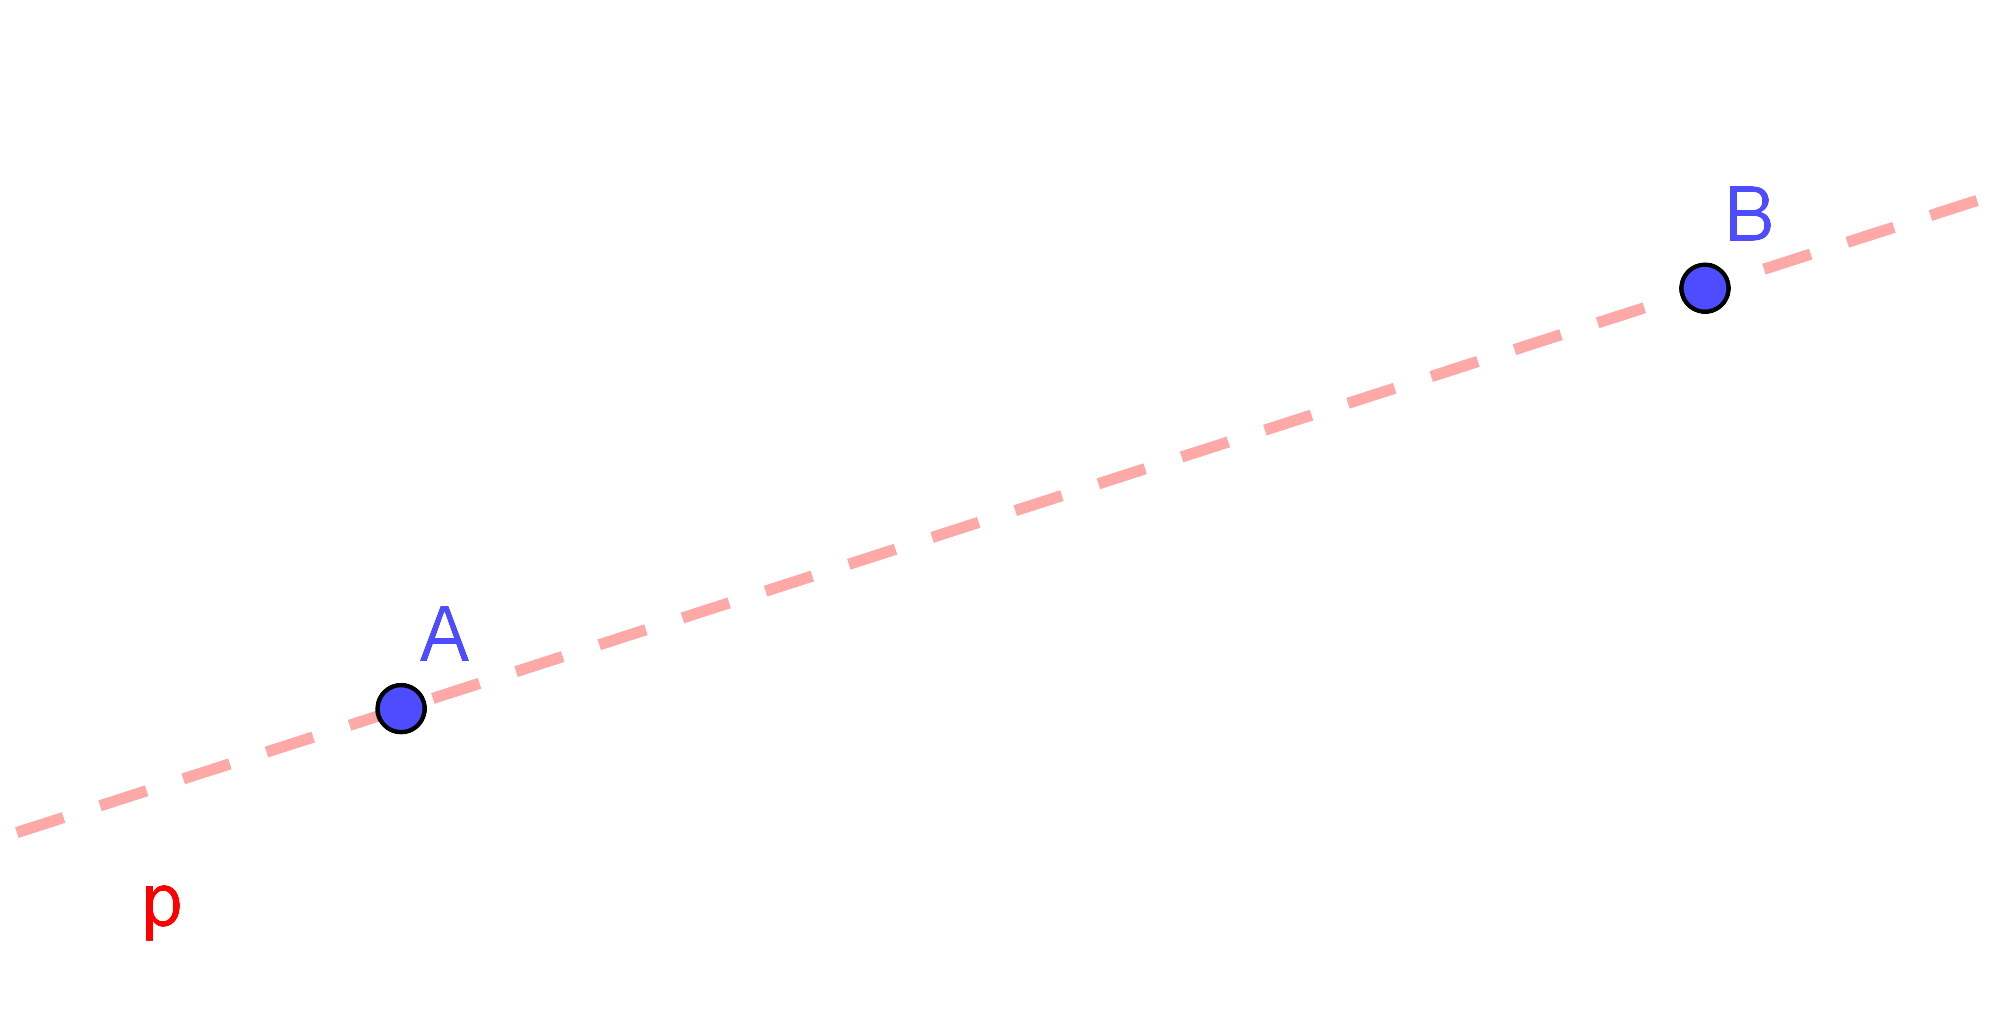
\includegraphics[width=0.4\textwidth]{images/origami_operacije/O1.png}
    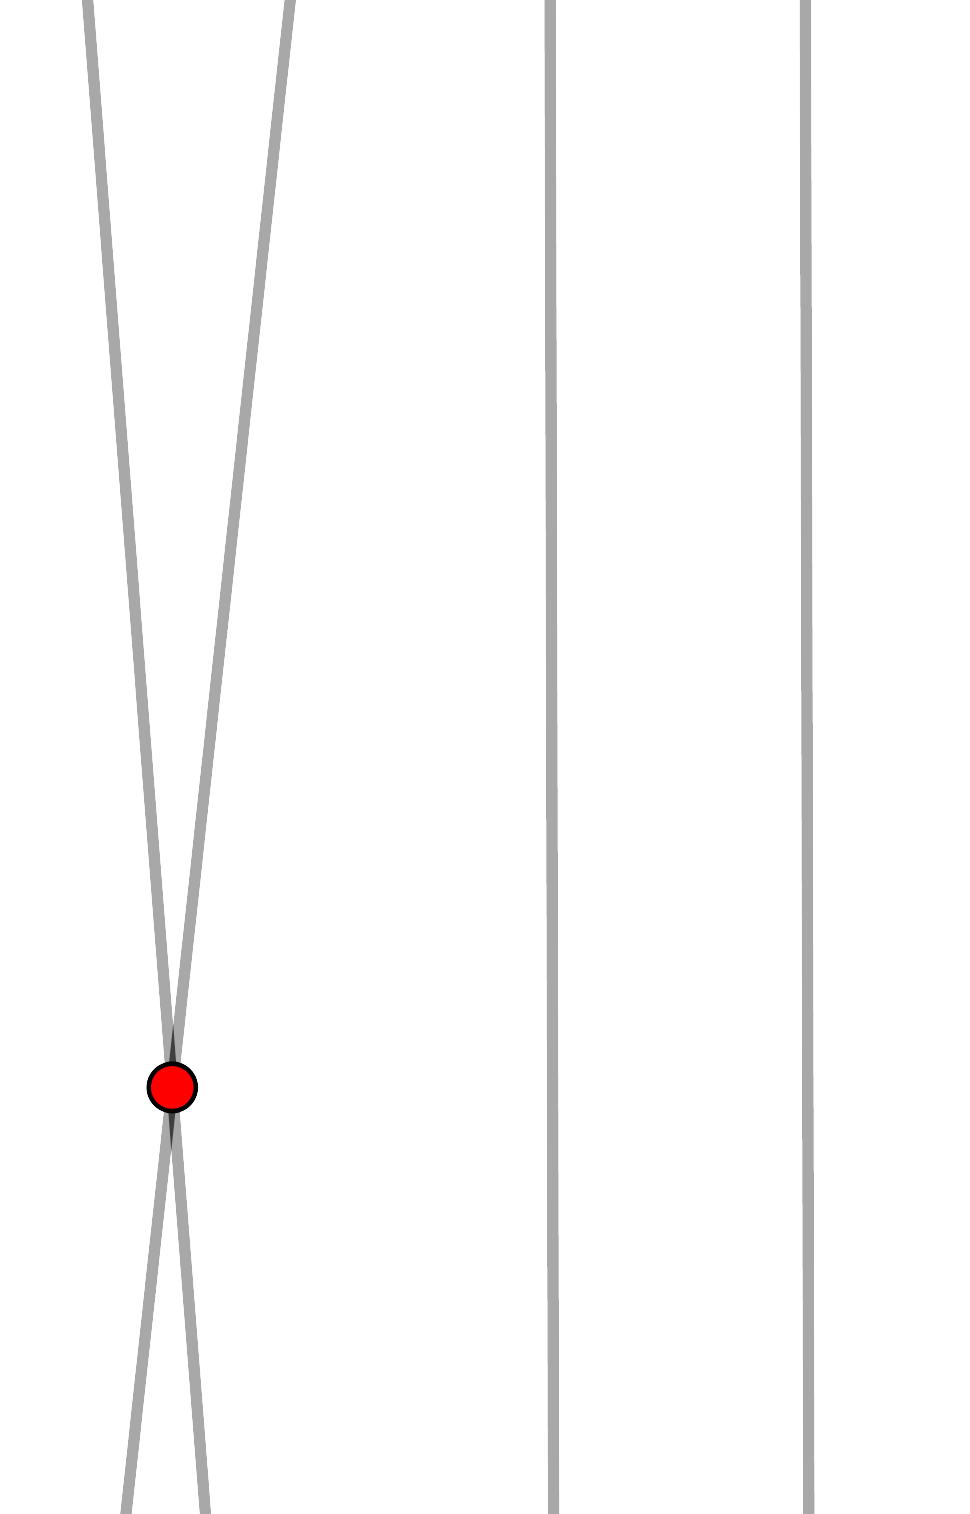
\includegraphics[width=0.2\textwidth]{images/origami_operacije/O2.png}
    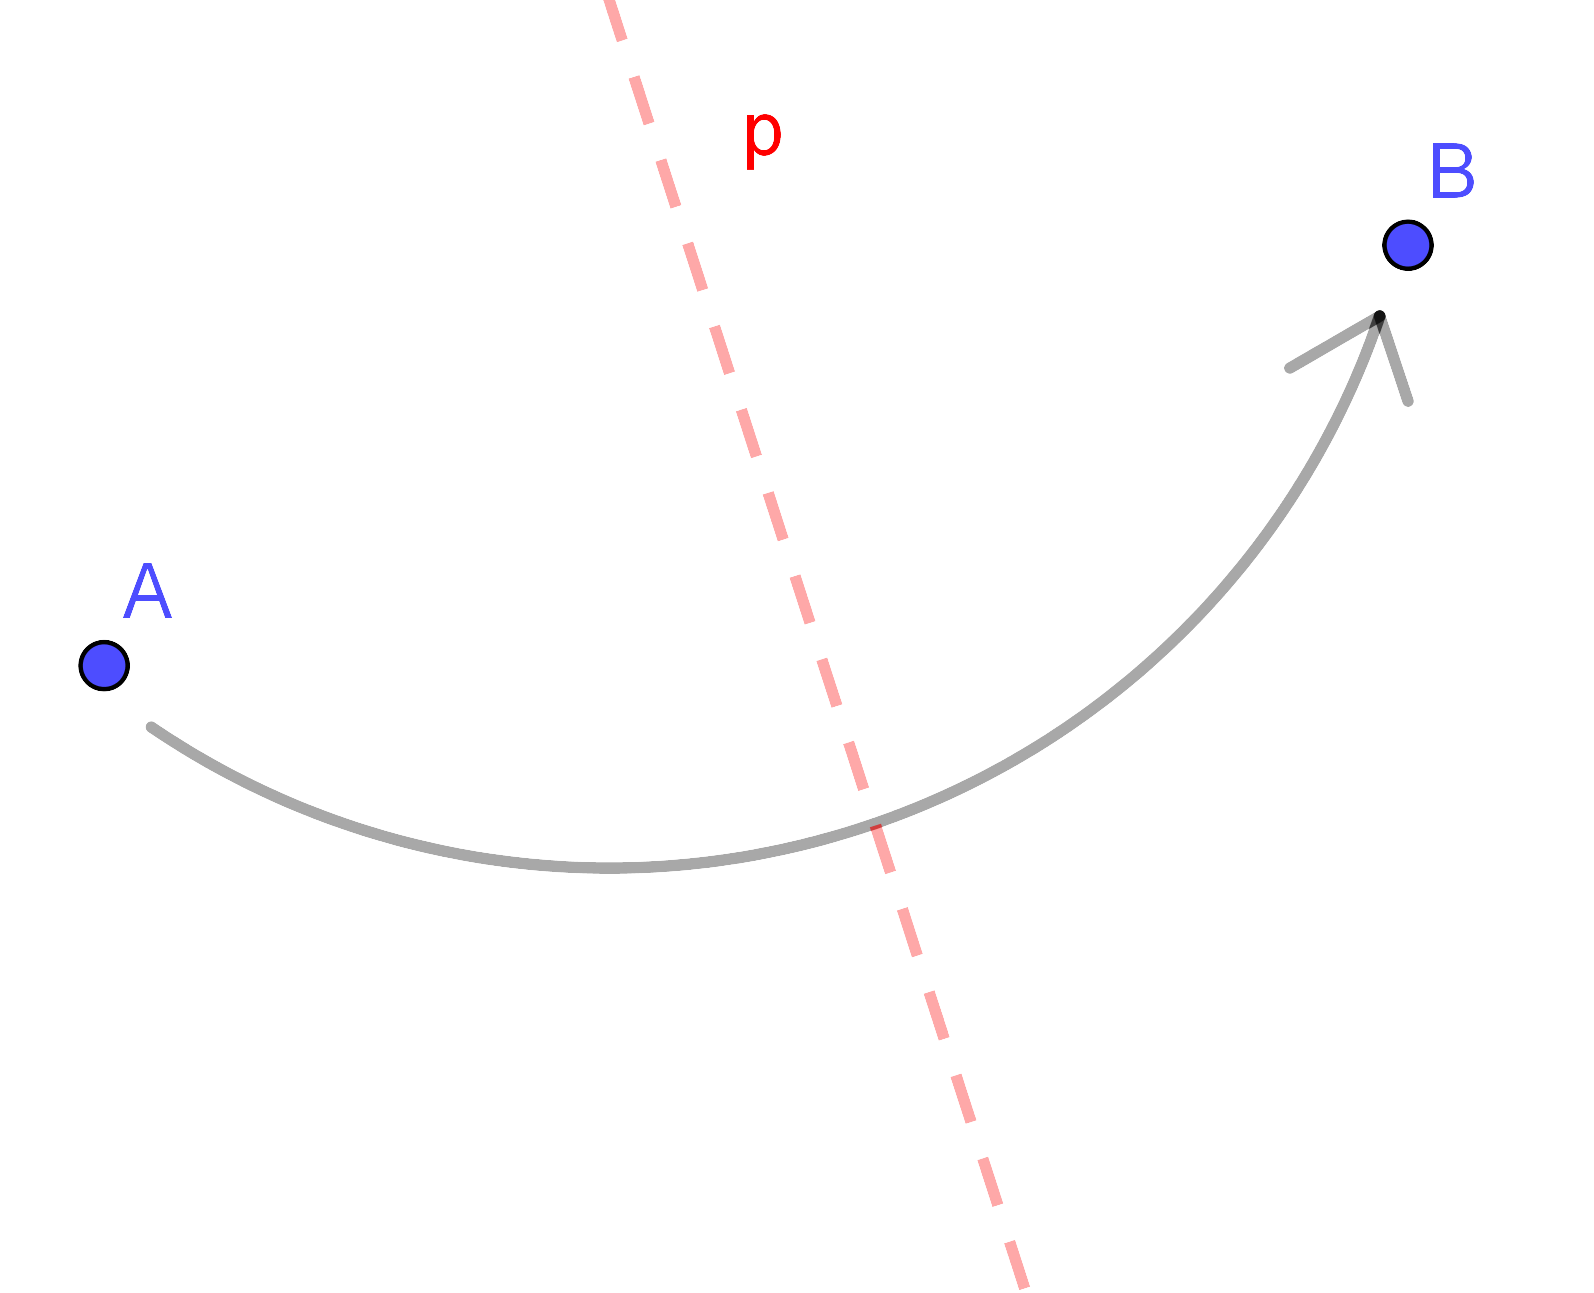
\includegraphics[width=0.35\textwidth]{images/origami_operacije/O3.png}
    \caption[Operacije~\ref{op:O1},~\ref{op:O2} in~\ref{op:O3}]{Operacije (od leve proti desni)~\ref{op:O1},~\ref{op:O2} in~\ref{op:O3}.}
    \label{fig:O1-O3}
\end{figure}

Nadalje opazimo, da nam operacija~\ref{op:O4} konstruira obe simetrali kota, ki ga določata premici in njuno presečišče, v primeru vzporednih premic pa dobimo tretjo vzporednico, ki leži na sredi med njima (slika~\ref{fig:O4}). Zato sta tu možna po dva ali, v posebnem primeru, en pregib.

\begin{figure}[h]
    \centering
    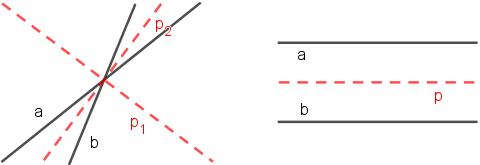
\includegraphics[width=0.5\textwidth]{images/origami_operacije/O4.png}
    \caption[Operacija~\ref{op:O4}]{Operacija~\ref{op:O4} v obeh možnih primerih.}
    \label{fig:O4}
\end{figure}

Operacija~\ref{op:O5} nam podaja konstrukcijo pravokotnice na premico skozi dano točko (slika~\ref{fig:O5}). Pri tem je vseeno, ali točka leži na premici ali ne. Pregib opravimo tako, da premico položimo samo nase in pazimo, da je točka $A$ v pregibu. Zaradi simetrije je pregib res pravokoten na premico in tako tudi en sam.

\begin{figure}[h]
    \centering
    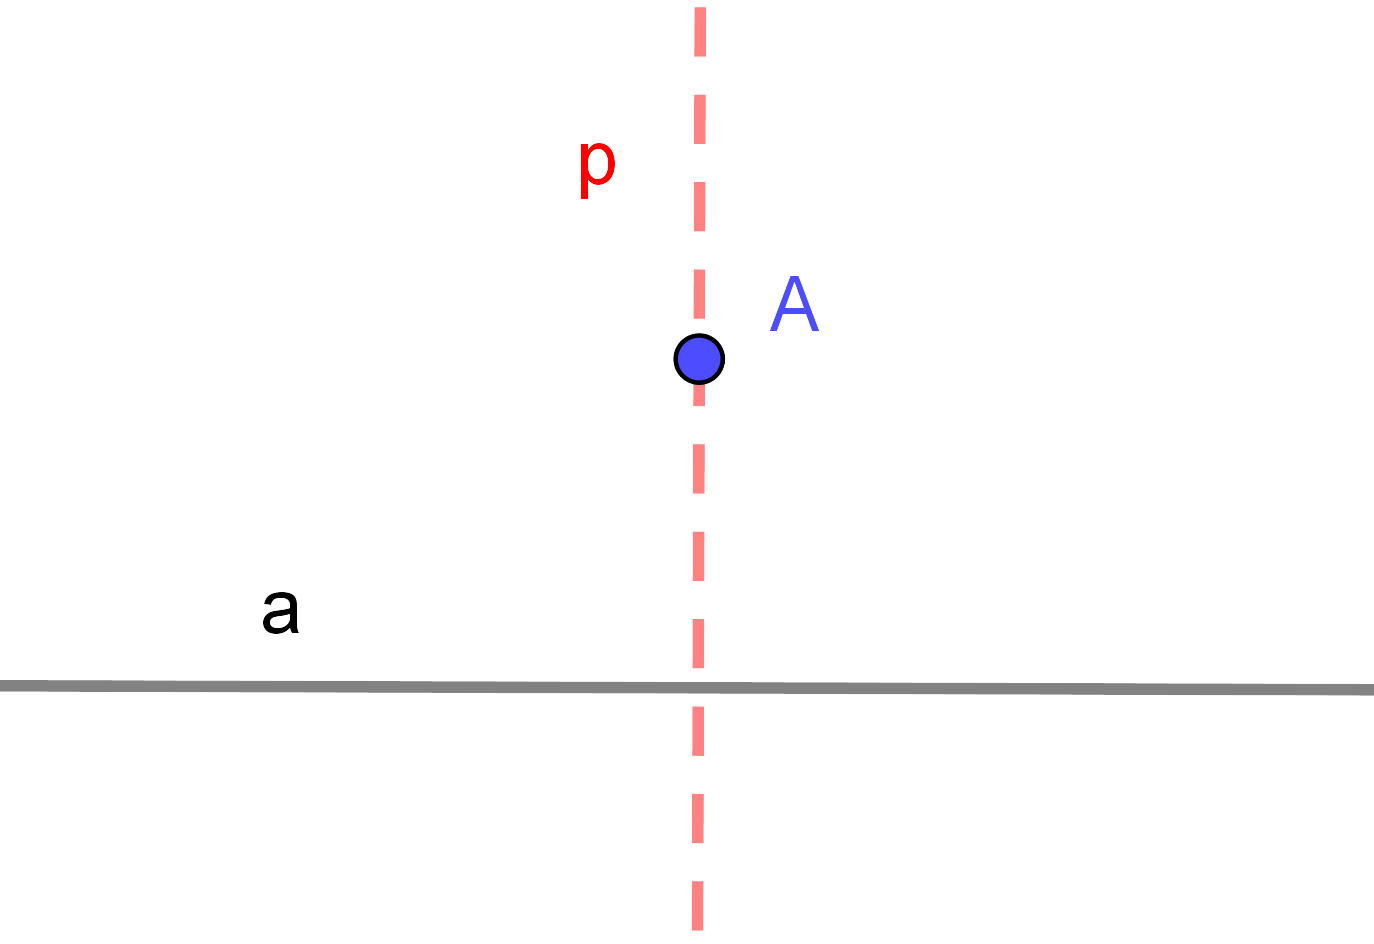
\includegraphics[width=0.35\textwidth]{images/origami_operacije/O5.png}
    \caption[Operacija~\ref{op:O5}]{Operacija~\ref{op:O5}.}
    \label{fig:O5}
\end{figure}

Operacija~\ref{op:O6} je še posebej zanimiva. Najprej si poglejmo njeno konstrukcijo. Vzemimo točki $A$ in $B$ ter premico $a$. Iščemo pregib skozi $B$, ki $A$ položi na premico $a$. Ker točka $B$ leži na pregibu, je enako oddaljena tako od točke $A$ kot tudi njene slike $A'$ na premici $a$, torej je $A'$ ravno presečišče premice $a$ in krožnice s središčem v $B$ ter polmerom $AB$. Pregib je simetrala daljice $AA'$, ki po konstrukciji poteka skozi točko $B$. Če velja $ d(A,B) > d(B,a) $, sta presečišči s premico $a$ dve (in s tem tudi dva možna pregiba, gl.\ sliko~\ref{fig:O6} levo), v primeru $ d(A,B) = d(B,a) $ je presečišče eno samo (in s tem en možen pregib, gl.\ sliko~\ref{fig:O6} na sredi) in je premica $a$ takrat tangentna na omenjeno krožnico, v zadnjem primeru, ko velja $ d(A,B) < d(B,a) $, pa presečišč ni (in s tem tudi pregiba, gl.\ sliko~\ref{fig:O6} desno).

\begin{figure}[h]
    \centering
    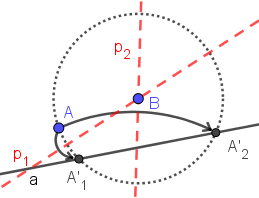
\includegraphics[width=0.55\textwidth]{images/origami_operacije/O6a.png}
    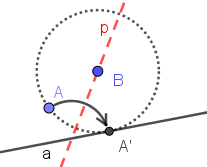
\includegraphics[width=0.2\textwidth]{images/origami_operacije/O6b.png}
    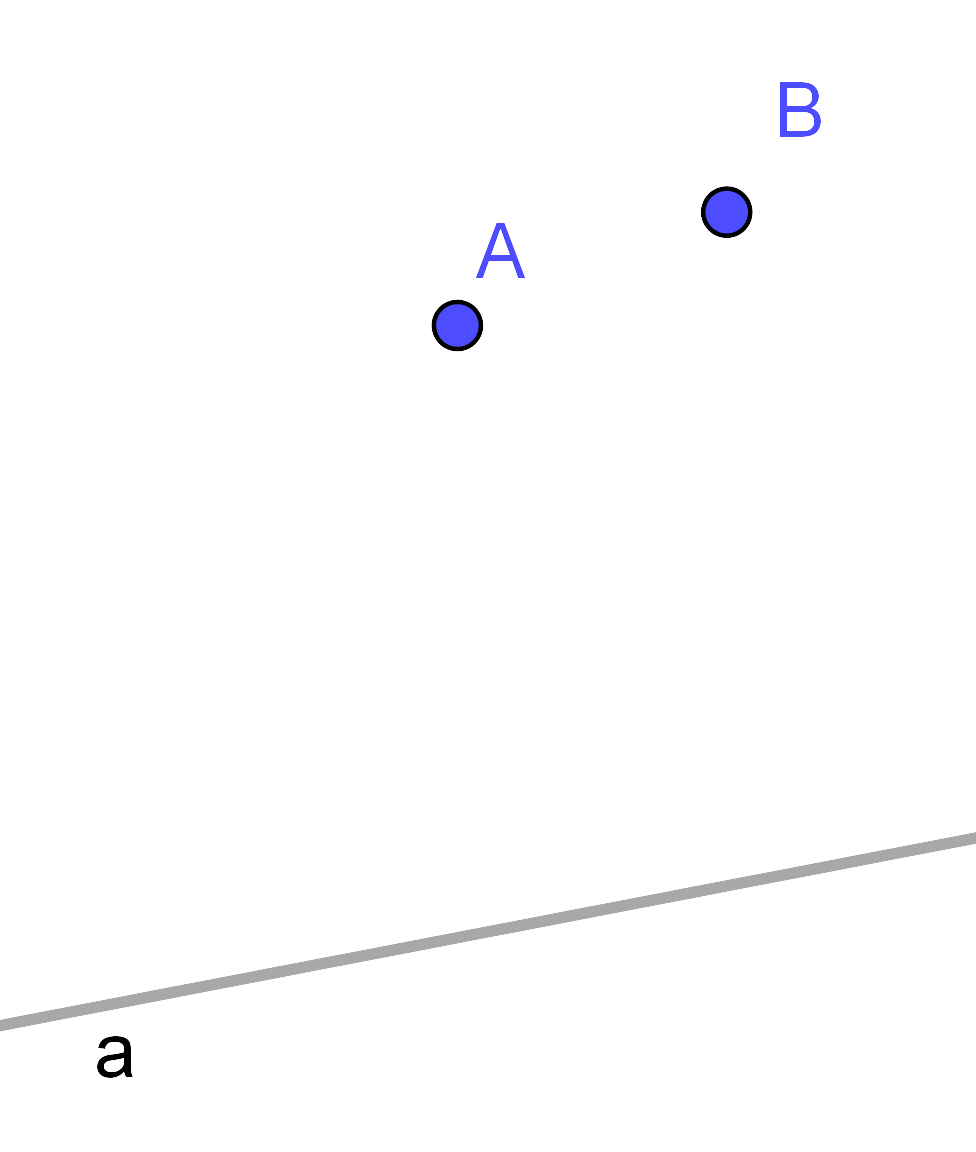
\includegraphics[width=0.2\textwidth]{images/origami_operacije/O6c.png}
    \caption[Operacija~\ref{op:O6}]{Operacija~\ref{op:O6} v vseh treh primerih.}
    \label{fig:O6}
\end{figure}

Zgodba operacije~\ref{op:O6} se tu še ne zaključi. Ker na pregibu ležijo vse točke, ki so enako oddaljene od točke $A$ in $A'$, to velja tudi za točko $P$, ki jo dobimo kot presečišče pregiba in pravokotnice na premico $a$ skozi $A'$ (slika~\ref{fig:O6_parabola}). Zanjo velja $ d(A,P) = d(P,a) $ in je enolično določena (v srednjem primeru na sliki~\ref{fig:O6} je to kar točka $B$). Torej točka $P$ leži na paraboli z goriščem $A$ in premico vodnico $a$. Bralec lahko sam premisli, da je $P$ edina točka na pregibu, ki je enako oddaljena od gorišča in premice vodnice. Pregib torej seka parabolo le v eni točki, kar pomeni, da je to \emph{tangenta na to parabolo}. V levem primeru na sliki~\ref{fig:O6} smo dobili dve tangenti.

\begin{figure}[h]
    \centering
    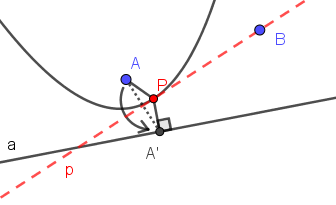
\includegraphics[width=0.6\textwidth]{images/origami_operacije/O6_parabola.png}
    \caption[Tangenta na parabolo]{Operacija~\ref{op:O6} kot konstrukcija tangente na parabolo z goriščem v $A$ in premico vodnico $a$.}
    \label{fig:O6_parabola}
\end{figure}

Poglejmo si naslednjo operacijo. Konstrukcijo~\ref{op:O7} začnemo z upogibom papirja, ki točko $A$ položi na premico $a$, potem pa točko premikamo po premici, dokler se tudi točka $B$ ne stakne s premico $b$. Takrat naredimo pregib. Za enako izbiro točk in premic je lahko možnih več pregibov (\textcolor{red}{(baje največ trije~\cite[str.\ 38 spodaj]{hull2020})}, gl.\ sliko~\ref{fig:O7}), če pa sta premici vzporedni in je njuna medsebojna razdalja večja od razdalje med točkama, pregib sploh ne obstaja -- pregib namreč razdaljo med točkama $A$ in $B$ ohrani, premici pa sta na večji medsebojni razdalji kot sta točki med seboj.

\begin{figure}[h]
    \centering
    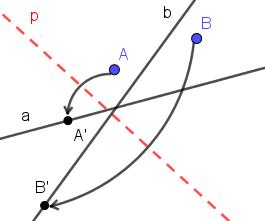
\includegraphics[width=0.35\textwidth]{images/origami_operacije/O7b.png}
    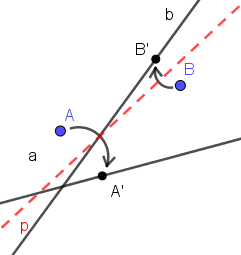
\includegraphics[width=0.3\textwidth]{images/origami_operacije/O7a.png}
    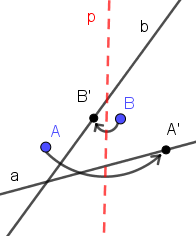
\includegraphics[width=0.3\textwidth]{images/origami_operacije/O7c.png}
    \caption[Operacija~\ref{op:O7}]{Operacija~\ref{op:O7} (primer treh pregibov za isti točki in premici).}
    \label{fig:O7}
\end{figure}

Kaj je geometrijski pomen te operacije? Če smo pri operaciji~\ref{op:O6} dobili tangento na parabolo, potem lahko takoj vidimo, da pri operaciji~\ref{op:O7} dobimo \emph{skupno tangento na dve paraboli} -- ena ima gorišče v točki $A$ in premico vodnico $a$, druga pa gorišče v točki $B$ ter premico vodnico $b$ (slika~\ref{fig:O7_paraboli}).

\begin{figure}[h]
    \centering
    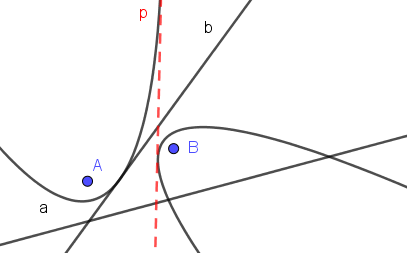
\includegraphics[width=0.7\textwidth]{images/origami_operacije/O7c_paraboli.png}
    \caption[Skupna tangenta na dve paraboli]{Operacija~\ref{op:O7} kot konstrukcija skupne tangente na dve paraboli.}
    \label{fig:O7_paraboli}
\end{figure}

\begin{opomba}
    O operaciji~\ref{op:O7} naj bi prva pisala italijanski matematičarki Margherita P.\ Beloch, po kateri operacijo imenujemo tudi \emph{Belochin pregib}.
\end{opomba}

Zadnja operacija~\ref{op:O8} zahteva nevzporedni premici, saj v nasprotnem primeru ne moremo konstruirati pregiba, ki bi bil pravokoten na obe premici in točko $A$ položil na premico $a$ (razen če le-ta že leži na njej). Premislimo geometrijsko konstrukcijo: ker mora biti pregib pravokoten na premico $b$, bo slika točke $A$ (označena z $A'$) ležala na vzporednici skozi točko $A$ k premici $b$. Prav tako mora točka $A'$ ležati na premici $a$, torej je slika ravno presečišče omenjene vzporednice in premice $a$. Iskan pregib je simetrala daljice $AA'$, ki je po konstrukciji pravokoten na premico $b$ (slika~\ref{fig:O8}).

\begin{figure}[h]
    \centering
    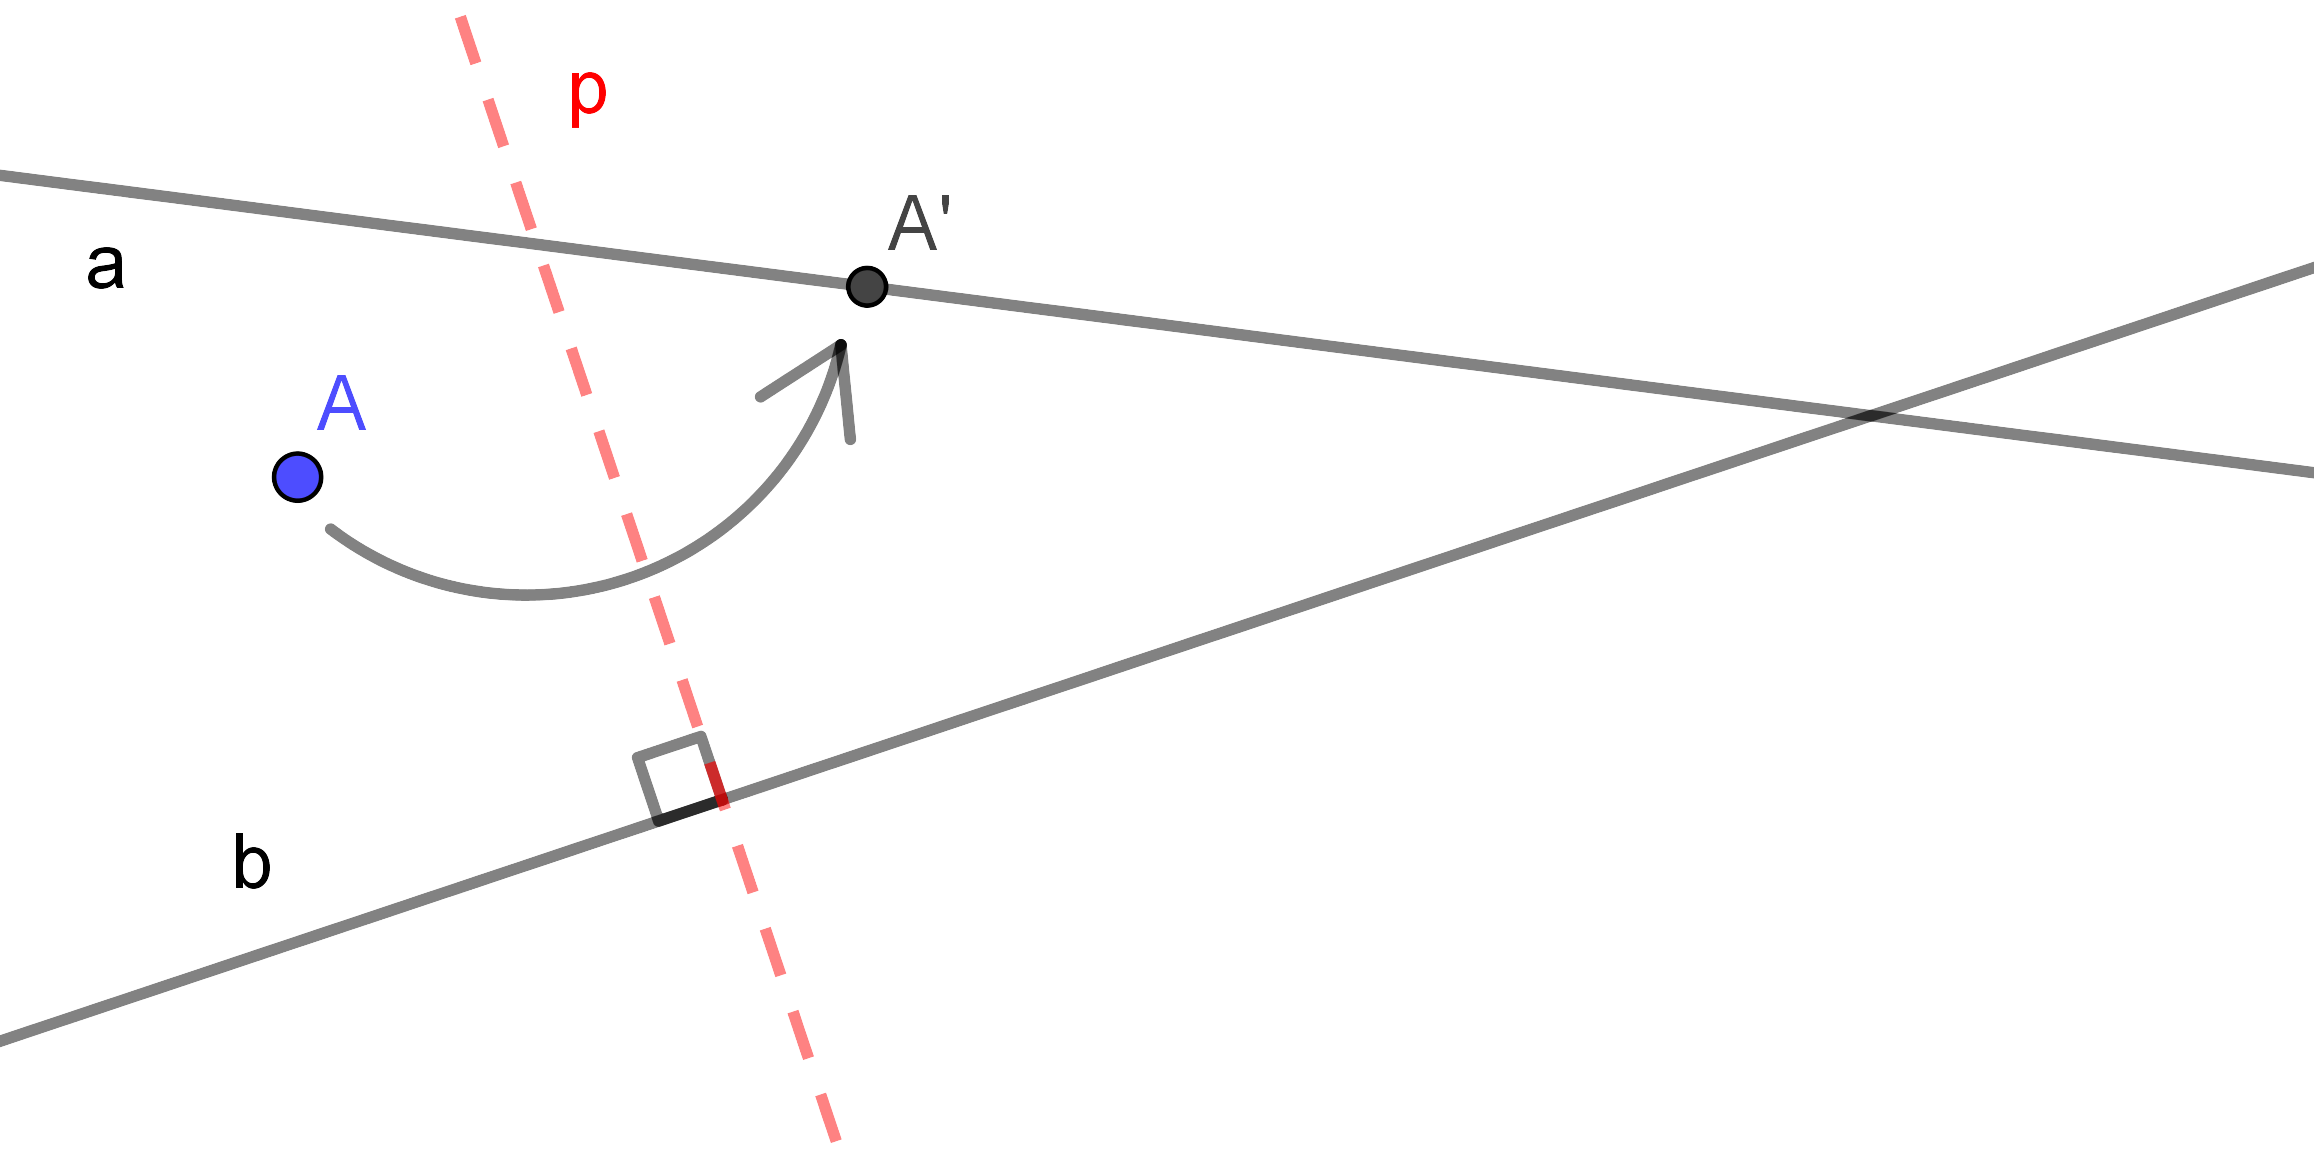
\includegraphics[width=0.6\textwidth]{images/origami_operacije/O8.png}
    \caption[Operacija~\ref{op:O8}]{Operacija~\ref{op:O8}.}
    \label{fig:O8}
\end{figure}

\opomba{Natančen bralec lahko opazi, da nam origami operacije ne podajajo konstrukcije slik točk, temveč samo pregibe, ki točke preslikajo na premice. Sliko točke konstruiramo šele po uporabi operacije~\ref{op:O5} -- skozi originalno točko naredimo pregib, pravokoten na prvi pregib (iz~\ref{op:O6}), in slika je potem presečišče pravokotnice in premice, na katero smo prepognili originalno točko.}

\subsubsection{Zadostne in potrebne origami operacije}

Izkaže se, da je teh osem operacij zadostnih za katerokoli origami konstrukcijo.

\begin{izrek}
    \label{izr:op1do8}
    Če dovolimo le enkratne in ravne pregibe, so edine možne operacije prepogibanja operacije~\ref{op:O1}--\ref{op:O8}.
\end{izrek}

Ideja dokaza je, da za vsak možen prepogib, ki prekrije točko ali premico s točko ali premico (gl.\ seznam na začetku podpoglavja \ref{origami_konstrukcije}) pogledamo vse možnosti. Izkaže se, da res dobimo prepogibe iz operacij~\ref{op:O1}--\ref{op:O8}. Za natančen dokaz s slikovno ponazoritvijo gl.\ \cite[str.\ 24--26 (izrek 1.1)]{hull2020}.

Vendar ali so vse te operacije tudi potrebne ali lahko kakšno izpustimo? Operacija~\ref{op:O2} je očitno potrebna, saj nam določa nove točke. Če podrobneje opazujemo ostale konstrukcije, pa opazimo, da so vse posebni primeri operacije~\ref{op:O7} (t.\ j.\ konstrukcija pregiba, ki točko $A$ položi na premico $a$ in točko $B$ na premico $b$), ko premici $a$ in $b$ sovpadata ali ko ena ali obe izmed točk $A$ in $B$ ležita na premici:
\begin{itemize}
    \item Operacija~\ref{op:O1}: Naj točka $A$ leži na premici $a$, točka $B$ pa na premici $b$. Pregib skozi točki $A$ in $B$ točko $A$ ohrani na premici $a$ in točko $B$ na premici $b$.
    \item Operacija~\ref{op:O3}: Naj točka $A$ leži na premici $b$, točka $B$ pa na premici $a$. Pregib, ki položi točki drugo na drugo, točko $A$ položi na premico $a$ in hkrati točko $B$ na premico $b$ .
    \item Operacija~\ref{op:O4}: Naj točka $A$ leži na premici $b$, točka $B$ pa na premici $a$. Simetrala kota v presečišču premic (ali vmesna vzporednica, če sta premici $a$ in $b$ vzporedni), točko $A$ položi na premico $a$ in hkrati točko $B$ na premico $b$.
    \item Operacija~\ref{op:O5}: Naj točka $A$ leži na premici $a$, točka $B$ pa na premici $b$. Pregib skozi točko $A$ (ali $B$), ki je pravokoten na premico $b$ (ali $a$), točko $A$ ohrani na premici $a$ in točko $B$ na premici $b$.
    \item Operacija~\ref{op:O6}: Naj točka $B$ leži na premici $b$. Pregib skozi točko $B$, ki točko $A$ preslika na premico $a$ (če tak pregib obstaja), točko $B$ ohrani na premici $b$.
    \item Operacija~\ref{op:O8}: Naj točka $B$ leži na premici $b$. Pregib, ki točko $A$ položi na premico $a$ in je pravokoten na premico $b$, točko $B$ ohrani na premici $b$.
\end{itemize}

Ker lahko vse konstrukcije po izreku~\ref{izr:op1do8} opišemo z operacijami~\ref{op:O1}--\ref{op:O8}, smo s tem dokazali spodnji izrek:

\begin{izrek}
    \label{izr:dve_operaciji}
    Če imamo dani vsaj dve točki in dve nevzporedni (lahko tudi identični) premici, ki vsebujeta dane točke, potem lahko vse origami konstrukcije z enkratnimi in ravnimi pregibi opišemo s kombinacijo operacij~\ref{op:O2} in~\ref{op:O7}.
\end{izrek}

Vseeno bomo ohranili vseh osem aksiom operacij, saj bomo kakšen pregib lažje razložili preko ene od ostalih petih operacij kot pa opisovali, na kakšen način je to operacija~\ref{op::O7}.

\subsubsection{Zrcaljenje točke čez premico}
\label{zrcaljenje_origami}

Operacija~\ref{op:O3} nam poda simetralo daljice $AB$. Torej je točka $B$ zrcalna slika točke $A$ čez to premico. Kaj pa, če imamo za neko točko $A$ že dano premico $a$ in iščemo njeno zrcalno sliko? Bralec bi lahko naivno predlagal, da naredimo pregib po premici in s svinčnikom označimo zrcalno sliko. A definicija~\ref{def:origami_konstruktibilnost} pravi, da lahko točke dobimo le kot presečišča pregibov, poleg tega pa je uporaba pisala dovoljena le za vidnejšo označbo že konstruiranih točk.

Zato moramo najti zaporedje pregibov, kjer na koncu kot presečišče nekih dveh premic dobimo želeno točko. Za dano premico $a$ in točki $A$, ki ne leži na tej premici (sicer je točka $A$ zrcalna slika sama sebi), lahko zrcalno sliko točke konstruiramo z naslednjimi koraki (prikazani na sliki~\ref{fig:zrcaljenje_cez_premico}, postopek vzet iz~\cite[str.\ 28]{hull2020}):
\begin{enumerate}
    \item Z operacijo~\ref{op:O5} prepognemo pravokotnico na premico $a$ skozi točko $A$.
    \item Z operacijo~\ref{op:O4} prepognemo simetralo kota, ki ga oklepata premica $a$ in pravokotnica iz prvega koraka.
    \item Z operacijo~\ref{op:O5} prepognemo pravokotnico na simetralo skozi točko $A$. Njeno presečišče s premico $a$ označimo z $B$.
    \item Z operacijo~\ref{op:O5} prepognemo pravokotnico na pregib iz tretjega koraka skozi točko $B$. Presečišče novega pregiba in pravokotnice iz prvega koraka označimo z $A'$.
\end{enumerate}

\begin{figure}[h]
    \centering
    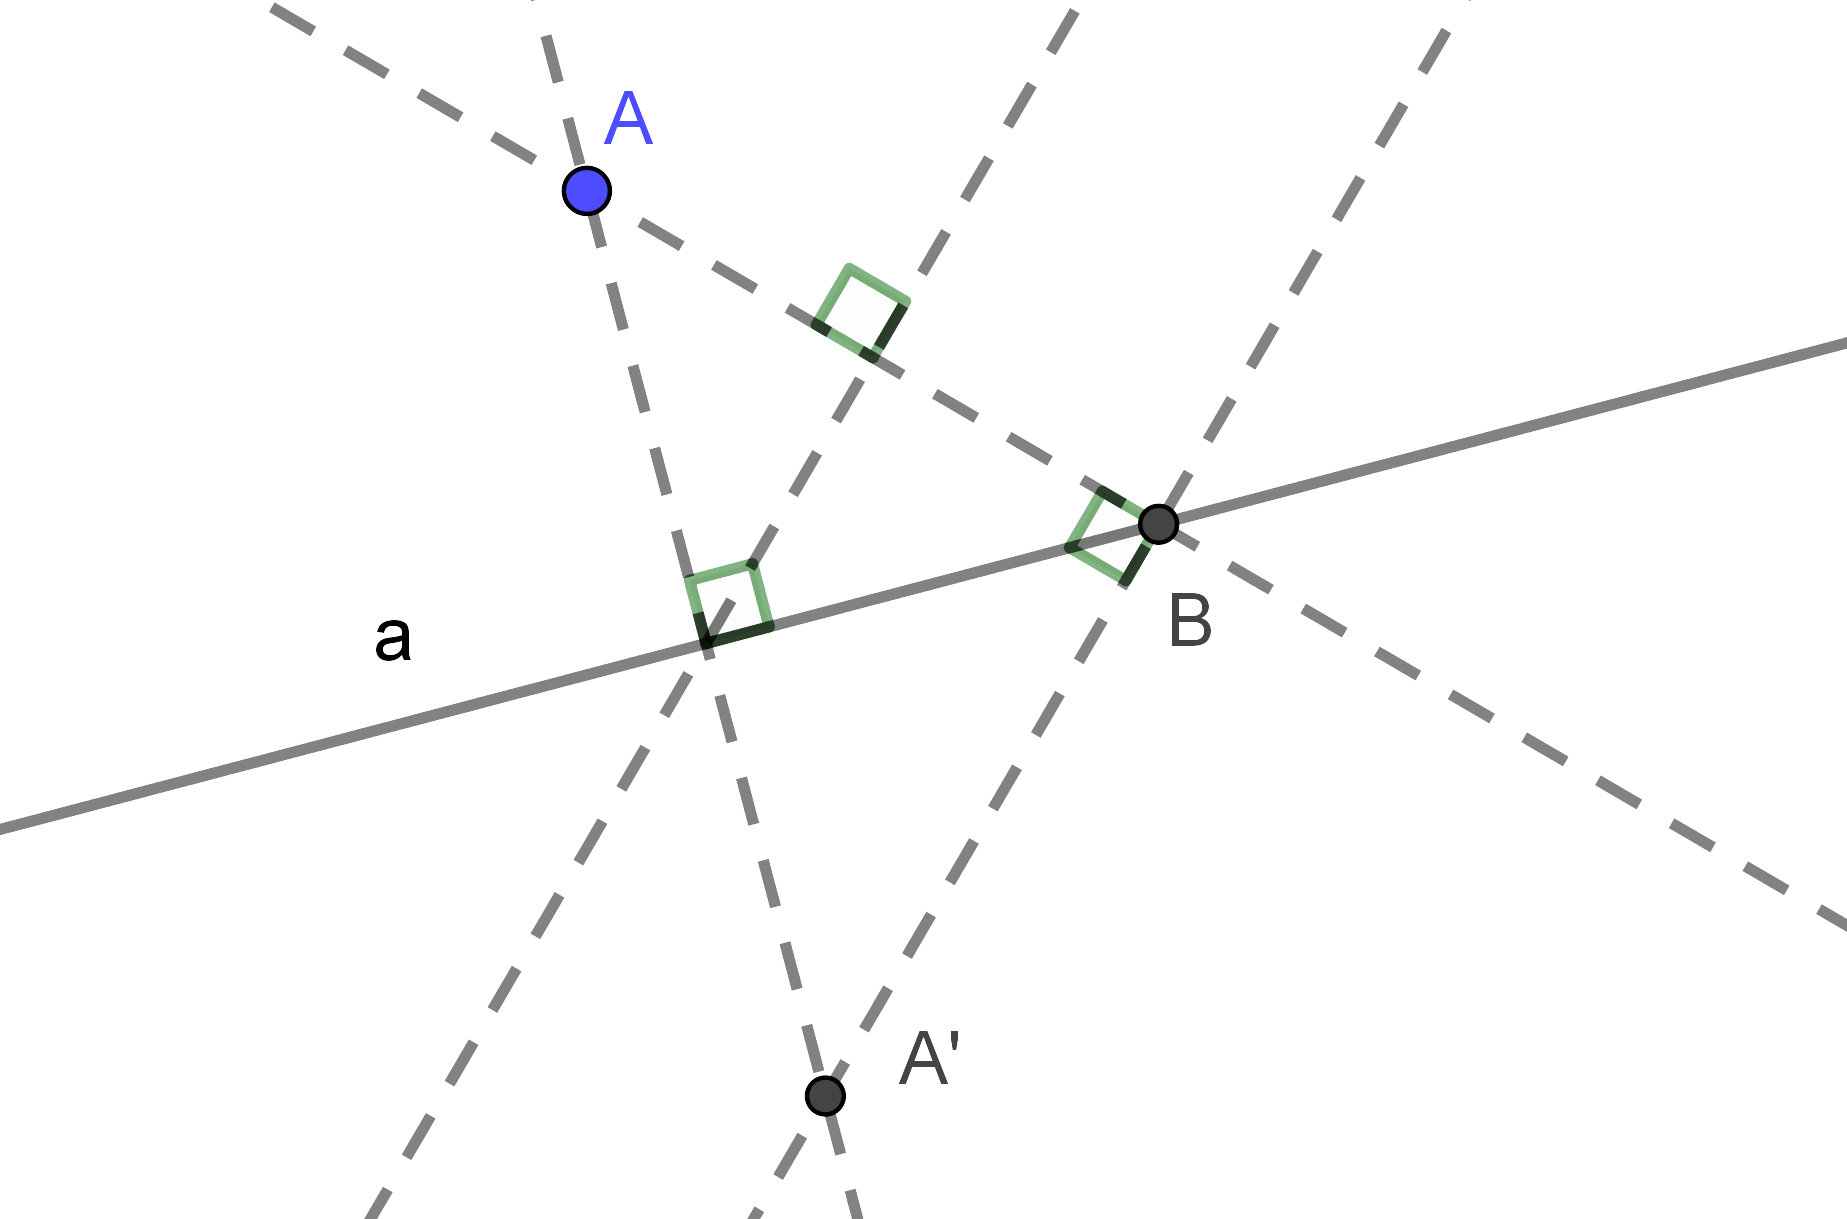
\includegraphics[width=0.5\textwidth]{images/zrcaljenje_tocke_cez_premico.png}
    \caption[Zrcaljenje čez premico]{Zrcaljenje točke $A$ čez premico $a$ s prepogibanjem papirja.}
    \label{fig:zrcaljenje_cez_premico}
\end{figure}

\begin{trditev}
    Točka $A'$ iz opisane konstrukcije je zrcalna slika točke $A$.
\end{trditev}

\begin{dokaz}
    Trikotnik, ki ga dobimo po 3.\ koraku, je pravokoten in enakokrak, saj je simetrala (pravega kota) iz 2.\ koraka pravokotna na njegovo osnovnico. Zato kot ob točki $A$ znaša $45^{\circ}$. Ker je trikotnik $\triangle A'BA$ pravokoten, je zato tudi enakokrak, torej premica $a$ razpolavlja daljico $AA'$, torej je $A'$ res zrcalna slika točke $A$.
\end{dokaz}

Ker lahko čez premico zrcalimo točke, lahko čeznjo zrcalimo tudi daljice oz.\ premice -- to storimo tako, da zrcalimo dve točki z daljice in naredimo pregib čez njuni sliki. Zrcaljenje pa nam omogoča še nekaj več, kar nam pove naslednja trditev.

% moja avtorska trditev in dokaz:)

\begin{trditev}
    \label{trd:prenasanje_razdalj}
    Z upoštevanjem pravil iz~\ref{origami_konstrukcije} in origami operacij lahko s prepogibanjem papirja prenašamo razdalje.
\end{trditev}

\begin{dokaz}
    V ravnini si izberimo poljubni točki $A$ in $B$, ki določata daljico z neko dolžino $r$. Naj bo $a$ poljubna premica in $A'$ poljubna točka na njej. Trditev pravi, da lahko z origami operacijami konstruiramo točko $B' \in a$, da je $d(A', B') =r$ (slika~\ref{fig:prenos_razdalje_konec}). Pri tem ni pomembno, na kateri strani točke $A'$ leži točka $B'$, saj jo lahko vedno zrcalimo čeznjo.

    \begin{figure}[h]
        \centering
        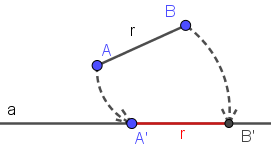
\includegraphics[width=0.5\textwidth]{images/zrcaljenje_konec.png}
        \caption[Prenašanje razdalj z origamijem]{Prenos dolžine daljice $AB$ na premico $a$ k izbrani točki $A'$.}
        \label{fig:prenos_razdalje_konec}
    \end{figure}
    
    Prenos razdalje razdelimo na dva koraka:
    \begin{enumerate}
        \item Če $A \ne A'$, daljico $AB$ zrcalimo čez tisto premico $p$, ki točko $A$ preslika v točko $A'$ (po~\ref{op:O3} je tak pregib oz.\ premica ena sama). Zrcalno sliko točke $B$ označimo z $B''$ (slika~\ref{fig:prenos_razdalje_koraki} levo). V posebnem primeru, ko daljica $AB$ leži na premici $a$, je to že konec konstrukcije. 
        \item Daljico $A'B''$ rotiramo okoli točke $A'$, da se točka $B''$ preslika na premico $a$. To storimo tako, da z operacijo~\ref{op:O4} konstruiramo simetralo kota med daljico $A'B''$ in premico $a$ in čeznjo zrcalimo točko $B''$ (slika~\ref{fig:prenos_razdalje_koraki} desno). S tem dobimo točko $B' \in a$, ki je po konstrukciji od točke $A'$ oddaljena za dolžino $r$.
    \end{enumerate}

    \begin{figure}[h]
        \centering
        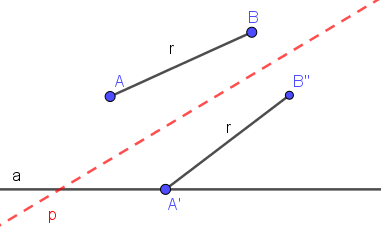
\includegraphics[width=0.45\textwidth]{images/zrcaljenje_korak1.png}
        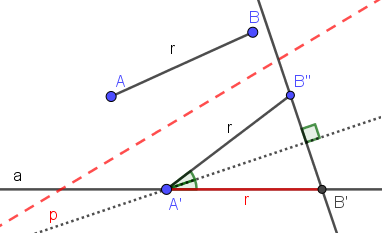
\includegraphics[width=0.45\textwidth]{images/zrcaljenje_korak2.png}
        \caption[Prenašanje razdalj z origamijem po korakih]{Zrcaljenje daljice $AB$ (levo) in rotacija daljice čez eno krajišče (desno).}
        \label{fig:prenos_razdalje_koraki}
    \end{figure}

    S tem smo razdaljo $r$ prenesli na poljubno mesto v ravnini.
\end{dokaz}

Tako lahko s prepogibanjem papirja zrcalimo točke (in premice), prenašamo razdalje pa tudi -- po 2.\ koraku iz zgornjega dokaza -- rotiramo točke (in premice). To novo znanje bomo uporabili v podpoglavju~\ref{origami_konstruktibilnost}. Od sedaj naprej bomo pri konstrukcijah, ki vključujejo zrcaljenje točk, zaradi preglednosti izpustili pregibe, ki so potrebni za zrcaljenje.

\subsection{Kje origami konstrukcije nadvladajo evklidske}
\label{podpogl:nadvlada_origamija}

Prišli smo do ključnega dela poglavja -- reševanje vprašanja, zakaj se nam z origami konstrukcijami sploh splača ukvarjati.

Za začetek naj bralec ob zgornjih opisih posamezne operacije premisli, da je mogoče operacije~\ref{op:O1}, \ref{op:O3}, \ref{op:O4}, \ref{op:O5}, \ref{op:O6} in \ref{op:O8} opraviti tudi z evklidskim orodjem (operacija~\ref{op:O2} le določa nove točke, zato tu o konstrukciji ne moremo govoriti). Do tu nam torej origami konstrukcije niso dale ničesar novega.

Ključna je sedma operacija. Izkaže se namreč, da operacije~\ref{op:O7} oz.\ Belochinega pregiba ne moremo opraviti z evklidskim orodjem. Prefinjen način, kako to dokazati, je preko rešitve starogrškega problema o trisekciji kota. V podpoglavju~\ref{podpogl:starogrskiproblemi} bomo spoznali več origami postopkov, ki nam poljuben kot razdelijo na tri skladne dele, pri tem pa uporabimo pregib iz operacije~\ref{op:O7}. Ker \emph{trisekcija kota z evklidskim orodjem ni mogoča} (dokaz v~\cite[str.\ 77--78]{jerman1998}), posledično tudi konstrukcija operacije~\ref{op:O7} s tem orodjem ne obstaja.

Tako z evklidskim orodjem kot s prepogibanjem papirja lahko torej konstruiramo premice in točke ter prenašamo razdalje. Le evklidskim orodjem lahko konstruiramo tudi krožne loke, le s prepogibanjem papirja pa lahko tretjinimo poljuben kot in še več kot to -- kot primer je uporaba Belochinega pregiba ključna za enega \textcolor{red}{(ali več???)} od postopkov reševanja kubičnih enačb, ki jih v splošnem z evklidskim orodjem ne moremo reševati (gl.\ poglavje~\ref{pogl:enacbe}).

Prednost origamija pred evklidskim orodjem je najbolj vidna, če evklidske in origami konstrukcije prevedemo v jezik abstraktne algebre.

\subsubsection{Algebrski pogled na evklidske konstrukcije}
\label{podpogl:evkl_konstruktibilnost}

\begin{definicija}
    Na listu papirja, ki nam služi kot model kompleksne ravnine $\C$, imejmo dano realno os, izhodišče $(0,0)$ in razdaljo 1. Če lahko le z neoznačenim ravnilom in šestilom konstruiramo točko $(x,0)$, rečemo, da je $x$ \emph{evklidsko-konstruktibilno} število. Pri tem upoštevamo tri pravila, ki izhajajo iz Evklidovih aksiomov in postulatov:
    \begin{itemize}
        \item točke dobimo kot presečišča dveh premic, dveh krožnic ali premice in krožnice,
        \item skozi vsaki točki lahko z ravnilom potegnemo ravno črto ter
        \item za vsako točko in razdaljo $r$ lahko s šestilom zarišemo krožnico, ki ima središče v tej točki in polmer $r$.
    \end{itemize}
\end{definicija}

\begin{opomba}
    Ker lahko uporabimo šestilo, ki prenaša razdalje (opomba~\ref{opom:solsko_sestilo}), je dovolj \emph{kjerkoli} v ravnini konstruirati točki z medsebojno razdaljo $x$.
\end{opomba}

Jerman bralca v~\cite{jerman1998} na zelo strukturiran in nazoren način popelje čez dokaz, da lahko z evklidskim orodjem konstruiramo natanko vsa racionalna števila, njihove vsote, razlike, zmnožke, količnike, kvadratne korene ter linearne kombinacije vsega naštetega. To je množica
$$
    \Q(r) = \{ a + b \sqrt{r}; a, b, r \in \Q; r > 0 \text{ in } \sqrt{r} \notin \Q \},
$$
ki je komutativen obseg oz.\ polje in hkrati tudi dvorazsežni vektorski prostor nad obsegom $\Q$ z bazo $ \{1, \sqrt{r} \} $.

Da pokažemo, da so to vsa možna evklidsko-konstruktibilna števila, je potrebna natančna obravnava vseh možnih enačb, ki jih dobimo pri iskanju presečišč dveh krožnic, dveh premic ter krožnice in premice, potem pa je potrebno še dokazati, da nam vse nadaljne rabe konstruiranih presečišč res podajo najmanjšo razširitev polja kompleksnih števil, ki je zaprta za operacijo kvadratnega korenjenja. Jerman s tem dokaže naslednji izrek.

\begin{izrek}
    \label{izr:evkl_konstr}
    Število $r \in \R$ se da konstruirati le s pomočjo ravnila in šestila natanko tedaj, ko je $r$ algebraičen nad $\Q$ in je razsežnost obsega $\Q(r)$, kot vektorskega prostora nad obsegom $\Q$, enaka $2^n$ za nek $n \in \N_0$.
\end{izrek}

\begin{opomba}
    \label{op:razseznost_obsega_evkl}
    Razsežnosti obsega $\Q(r)$ pravimo tudi \emph{stopnja razširitve obsega $\Q$}. Izkaže se, da je enaka stopnji minimalnega polinoma števila $r$ nad $\Q$~\cite[str.\ 77]{jerman1998}.
\end{opomba}

Izreku takoj sledita dokaza, da trisekcija kota v splošnem ter konstrukcija števila $ \sqrt[3]{2} $ z evklidskim orodjem nista mogoči~\cite[str.\ 77--78]{jerman1998}.

Iz izreka sledi tudi, da lahko vsa evklidsko-konstruktibilna števila analitično zapišemo kot rešitve kvadratne enačbe z racionalnimi koeficienti. O reševanju enačb se bomo natančneje ukvarjali v poglavju~\ref{pogl:enacbe}.

\subsubsection{Števila, konstruktibilna z origamijem}
\label{origami_konstruktibilnost}

Poiščimo še množico števil, ki jih lahko konstruiramo z origamijem.

\begin{definicija}
    Na listu papirja, ki nam služi kot model ravnine $\R^2$, imejmo dano abscisno os, izhodišče $(0,0)$ in točko $(1,0)$. Če lahko le z enkratnimi ravnimi prepogibi konstruiramo točko $(x,0)$, rečemo, da je $x$ \emph{origami-konstruktibilno} število. Pri tem upoštevamo pet pravil iz začetka podpoglavja~\ref{origami_konstrukcije}.
\end{definicija}

\begin{opomba}
    Vemo že, da operacije~\ref{op:O1}--~\ref{op:O8} zajamejo vse možne pregibe iz teh petih pravil, zato se jih še naprej poslužujmo.
\end{opomba}

\begin{opomba}
    Ker znamo konstruirati pravokotnice in prenašati razdalje (trditev~\ref{trd:prenasanje_razdalj}), lahko predpostavimo, da imamo dan kar celotnen koordinatni sistem z abscisno in ordinatno osjo, izhodiščem ter enoto $1$ na obeh oseh. Zato je tudi dovolj \emph{kjerkoli} v ravnini konstruirati točki z medsebojno razdaljo $x$.
\end{opomba}

\begin{izrek}
    \label{izr:origami_konstruktibilnost}
    Za poljuben $r \in \Q^{+}, \sqrt{r} \notin \Q$, so origami-konstruktibilna vsa števila iz množice $\Q(r) = \{a + b\sqrt{r}; a, b \in \Q\}$.
\end{izrek}

\begin{dokaz}
    Ekvivalentno to pomeni, da lahko konstruiramo realne rešitve poljubne kvadratne enačbe, saj je njena splošna rešitev ravno oblike $a + b\sqrt{r} $ za neke $ a, b \in \Q$ in $r \in \Q^{+}$. Torej moramo dokazati, da znamo s prepogibanjem seštevati, odštevati, množiti, deliti in koreniti dana oz.\ že konstruirana števila.
    
    Na začetku imamo dani točki $(0, 0)$ in $(1, 0)$, ki predstavljata števili 0 in 1. Brez težav lahko za poljuben $x \in \Z$ konstruiramo točko $(x, 0)$, saj znamo zrcaliti točke čez premice in prenašati razdalje. Zato je tudi seštevanje in odštevanje že konstruiranih števil enostavno. Deljenje je podrobneje obravnavano v poglavju~\ref{pogl:prepog_kvadrata}, kjer bomo spoznali, kako neko dolžino s prepogibanjem razdeliti na $n$ delov za poljubni $n \in \N$. S tem znanjem in uporabo množenja (ki je poseben primer seštevanja) lahko torej konstruiramo poljuben $x \in \Q$ oz.\ poljubno točko $(x, y)$ z racionalnima koordinatama v ravnini. Obstaja pa tudi več bolj direktnih metod za konstrukcijo števila $a/b \in \Q$ (glej~\cite[str.\ 12--21]{lang2013}).
    
    Manjka nam samo še konstrukcija kvadratnega korena poljubnega racionalnega števila. V ta namen si poglejmo naslednjo konstrukcijo (vzeto iz~\cite[str.\ 58]{hull2013}):
    Imejmo točko $A (0, 1) $, premico $y = -1$ in poljuben $r \in \Q^{+}$ (po zgornjem premisleku jih znamo konstruirati). Na ordinatni osi označimo točko $B (0, -\frac{r}{4})$ in naredimo pregib skoznjo, ki točko $A$ položi na premico $y = -1$. Njena zrcalna slika je $A' (t, 0) $ za nek $t \in \R$ (slika~\ref{fig:konstrukcija_korena}).
    
    \begin{figure}[h]
        \centering
        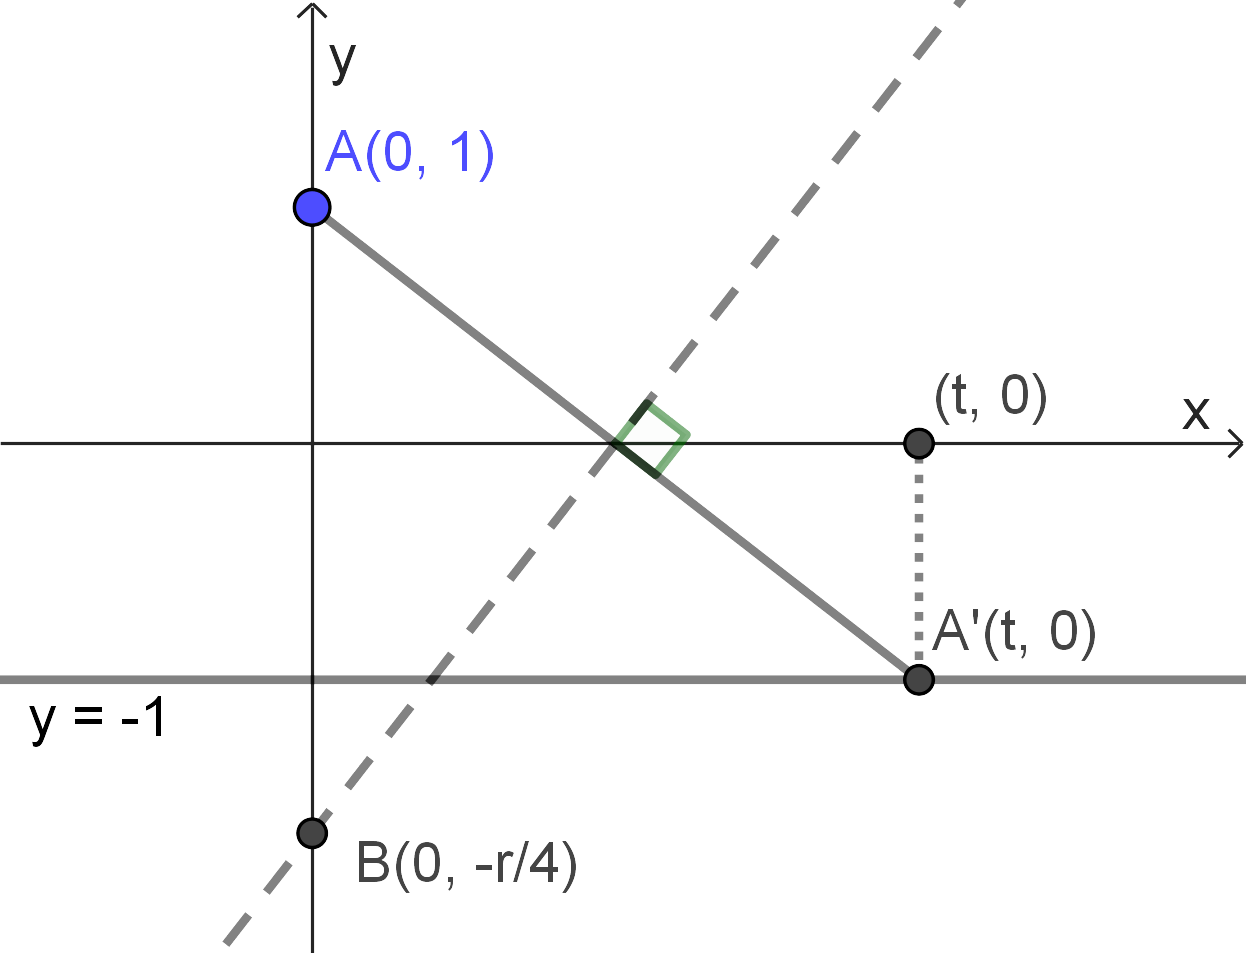
\includegraphics[width=0.5\textwidth]{images/kvadratni_koren.png}
        \caption[Konstrukcija korena]{Konstrukcija števila $\sqrt{r}$ za poljuben $r \in \Q^{+}$.}
        \label{fig:konstrukcija_korena}
    \end{figure}
    
    Pregib poteka skozi točko $B$ in razpolovišče daljice $AA'$, torej je njegov koeficient $k_B = \frac{r}{2t}$ (izpeljavo prepuščamo bralcu). Ker je pregib simetrala daljice $AA'$, njena nosilka pa ima koeficient $k_A = - \frac{2}{t}$, dobimo enačbo
    \begin{align*}
        k_B &= - \frac{1}{k_A}\\
        \frac{r}{2t} &= \frac{t}{2}\\
        r &= t^2 \text{ oz. } t = \sqrt{r}.
    \end{align*}
    Na koncu le še prepognemo pravokotnico na abscisno os skozi točko $A'$ in tako dobimo točko $(\sqrt{r}, 0)$. Torej smo konstruirali število $\sqrt{r}$ za poljuben $r \in \Q^{+}$.
\end{dokaz}

\begin{opomba}
    V razdelku~\ref{podpogl:kvadratna_enacba} bomo pokazali, kako s prepogibanjem rešimo poljubno kvadratno enačbo z racionalnimi koeficienti brez pomoči kvadratne formule, kar je v bistvu še en dokaz zgornjega izreka.
\end{opomba}

\begin{posledica}
    \label{posl:evkl_origami_konstruktibilnost}
    Vsa evklidsko-konstruktibilna števila so origami-konstruktibilna.
\end{posledica}

Do tega zaključka lahko pridemo tudi intuitivno. Operacija~\ref{op:O1} simulira uporabo neoznačenega ravnila, konstrukcija v operaciji~\ref{op:O6} podaja točke, ki so enako oddaljene od nekega središča, kar je ravno namen šestila.

Kot smo omenili že na začetku razdelka~\ref{podpogl:nadvlada_origamija}, se da s prepogibanjem konstruirati \emph{še kaj več} kot z evklidskim orodjem. Poleg trisekcije poljubnega kota in reševanja kubičnih enačb med drugim lahko med drugim konstruiramo tudi $\sqrt[3]{k} $ za poljuben\footnote{Za $k = 2$ je to rešitev starogrškega problema o podvojitvi kocke. Več o tem sledi v podpoglavju~\ref{podpogl:starogrskiproblemi}} konstruktibilen $k$ (dokaz v~\cite[str.\ 156]{geometricconstructions}). Prepogibanje papirja je torej res močnejše orodje od evklidskega.
\newpage
\section{Prepogibanje kvadrata}
\label{pogl:prepog_kvadrata}

Vzemimo v roke kvadraten list papirja in poglejmo, kaj lahko z njegovim prepogibanjem dobimo. V tem poglavju se bomo ukvarjali s preprostimi konstrukcijami, kot so konstrukcija enakostraničnega trikotnika in števila $\sqrt{r}$ za poljuben $r \in \mathcal{O}$. Pogledali si bomo vse tri Hagove izreke o razmerjih, na katere specifični pregibi kvadratnega lista papirja razdelijo njegove stranicE, nato pa to posplošili na iskanje metod za razdelitev daljice na poljubno število skladnih delov. Na koncu pa bomo končno preko več različnih konstrukcij rešili dva starogrška problema, zaradi katerih smo se sploh začeli ukvarjati s temo origamija.

\subsection{Nekaj kratkih in zanimivih konstrukcij za uvod}

\subsubsection*{Konstrukcija enakostraničnega trikotnika}

- kot 60° (smo že pri algebri)
- enakostranični trikotnik (smo že pri algebri, ma lahko še enkrat, pa več načinov)

\subsubsection*{Konstrukcija števila $\sqrt{r}$}

\textcolor{red}{Tu ne rabiš kvadratnega lista!}

Vzemimo $r \in \Q^+$ in si poglejmo naslednjo konstrukcijo (vzeto iz~\cite[str.\ 58]{hull2013}):
Imejmo točko $A (0, 1) $ in premico $y = -1$. Na ordinatni osi označimo točko $B (0, -r/4)$ in z operacijo~\ref{op:O6} skoznjo naredimo pregib, ki točko $A$ položi na premico $y = -1$. Njena zrcalna slika je $A' (t, 0) $ za nek $t \in \R$ (slika~\ref{fig:konstrukcija_korena}).

\begin{figure}[h]
    \centering
    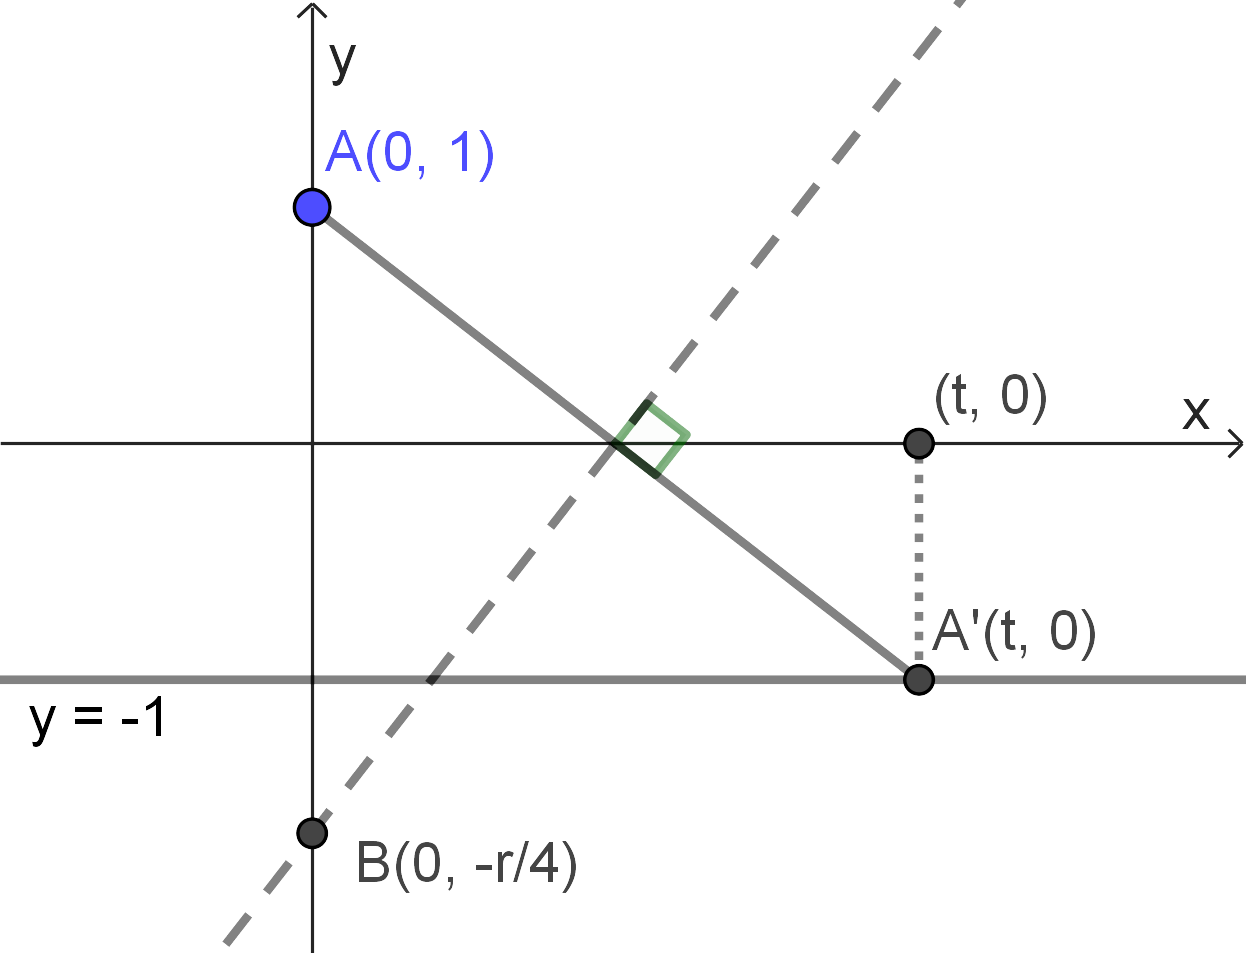
\includegraphics[width=0.5\textwidth]{images/kvadratni_koren.png}
    \caption[Konstrukcija korena]{Konstrukcija števila $\sqrt{r}$ za poljuben $r \in \Q^{+}$.}
    \label{fig:konstrukcija_korena}
\end{figure}

Pregib po konstrukciji poteka skozi točko $B$ in razpolovišče daljice $AA'$, torej je njegov koeficient $k_B = \frac{r}{2t}$ (izpeljavo prepuščamo bralcu). Ker je pregib simetrala daljice $AA'$, njena nosilka pa ima koeficient $k_A = - \frac{2}{t}$, dobimo
\begin{align*}
    k_B &= - \frac{1}{k_A},\\
    \frac{r}{2t} &= \frac{t}{2},\\
    r &= t^2 \text{ oz. } t = \sqrt{r}.
\end{align*}
Na koncu le še prepognemo pravokotnico na abscisno os skozi točko $A'$ in tako dobimo točko $(\sqrt{r}, 0)$. Torej smo konstruirali število $\sqrt{r}$ za poljuben $r \in \Q^{+}$.

\textcolor{red}{Še kakšna konstrukcija?}

\subsection{Hagovi izreki}

S prepogibanjem kvadratnega lista papirja se je veliko ukvarjal Kazuo Haga, sicer japonski profesor biologije. V svojem delu \emph{Origamics: Mathematical Explorations Through Paper Folding}~\cite{haga2008} je tako med drugim formuliral tri izreke, ki jih poznamo pod imenom \emph{Hagovi izreki}. Pri vsakem od njih gre za konstrukcijo specifičnega pregiba, ki povzroči delitev stranic kvadrata v različnih razmerjih. Vsak izrek posebej bomo najprej formulirali, si slikovno ogledali konstrukcijo in ga dokazali, nato pa si pogledali še nekaj dodatnih lastnosti, ki sledijo iz njega.

Da si olajšamo računanje, predpostavimo, da ima kvadrat, ki predstavlja naš list papirja, stranico dolžine $1$. Njegova oglišča označimo s črkami $A, B, C$ in $D$, začenši v zgornjem desnem oglišču in sledečimi v pozitivni smeri, torej nasprotni smeri urinega kazalca.

\textcolor{red}{Konstrukcija poljubnega $a/b \in \Q$~\cite[str.\ 20--21]{lang2013}}

\textcolor{red}{Hull2013, activity 11 (str. 103--)}

\subsubsection{Prvi Hagov izrek}

\begin{izrek}[Prvi Hagov izrek]
    Zgornjo stranico $AD$ kvadrata $ABCD$ razpolovimo v točki $E$ in s pregibom nanjo položimo oglišče $C$. S tem na levi in desni stranici kvadrata dobimo tri točke, ki jih označimo z $F, G$ in $H$ (slika~\ref{fig:hagov_izrek1}). Za te točke velja:
    \begin{itemize}
        \item točka $F$ deli desno stranico v razmeru $3:5$,
        \item točka $H$ deli levo stranico v razmerju $2:1$,
        \item točka $H$ deli spodnjo stranico v razmerju $1:5$,
        \item točke $G$ deli levo stranico v razmerju $7:1$.
    \end{itemize}
\end{izrek}

\begin{figure}[h]
    \centering
    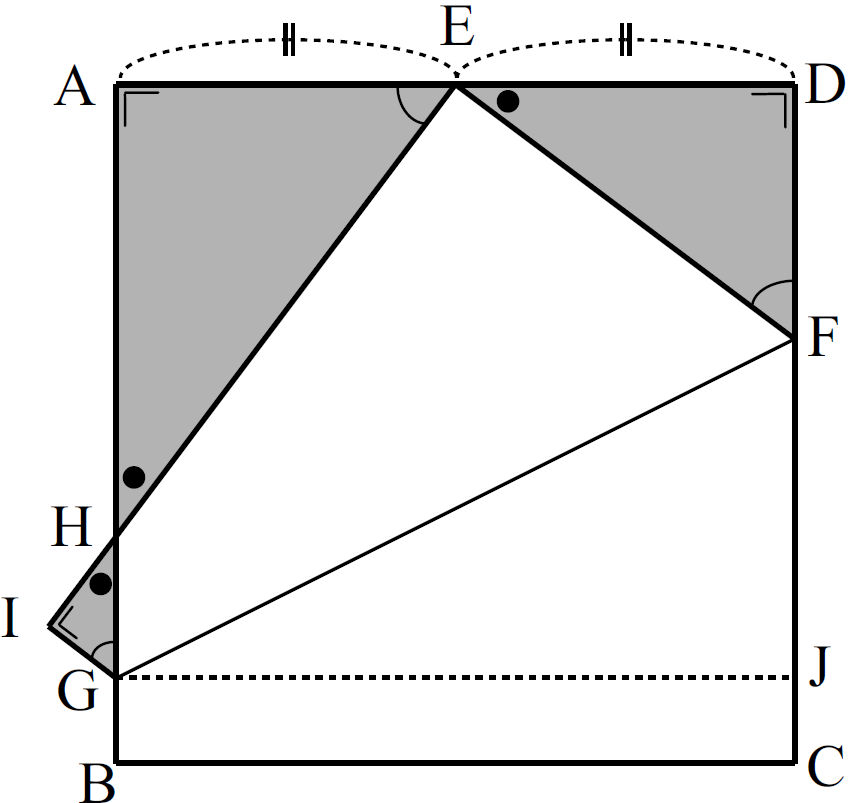
\includegraphics[width=0.45\textwidth]{images/hagovi_izreki/hagov_izrek1.png}
    \caption[Pregib iz prvega Hagovega izreka]{Konstrukcija pregiba iz prvega Hagovega izreka. Vzeto iz~\cite[str. 4]{haga2008}.}
    \label{fig:hagov_izrek1}
\end{figure}

\begin{dokaz}
    Kot kaže slika~\ref{fig:hagov_izrek1}, označimo še točki $I$ in $J$. Najprej lahko opazimo, da pregib iz izreka povzroči nastanek treh podobnih pravokotnih trikotnikov, ki so na sliki~\ref{fig:hagov_izrek1} pobarvani sivo. Za vsakega od njih lahko določimo dolžine njegovih stranic.

    Začnimo s trikotnikom $\triangle DEF$. Ker je $E$ razpolovišče stranice $AD$, je $|DE| = 1/2$. Če drugo kateto $DF$ označimo z $a$, je hipotenuza $EF$ dolga $1-a$, saj $|DF| + |EF| = |DF| + |FC| = 1$ po konstrukciji. Iz Pitagorovega izreka nato izračunamo $a = 3/8$. Torej točka $F$ res deli stranico $CD$ v razmerju $3:5$.

    Iz razmerja podobnih trikotnikov $\triangle DEF$ in $\triangle AHE$ dobimo
    $$ \frac{|AH|}{|AE|} = \frac{|DE|}{|DF|}, \; \text{ torej } \; |AH| = \frac{|AE|\cdot|DE|}{|DF|} = \frac{1/2 \cdot 1/2}{3/8} = \frac{2}{3}.$$
    Točka $H$ res deli stranico $AB$ v razmerju $2:1$. Drugače povedano -- s prvim Hagovim izrekom znamo poljubno daljico razdeliti na tri skladne dele.

    Sedaj lahko izračunamo dolžino hipotenuze $EH$ trikotnika $\triangle AHE$. Iz Pitagorovega izreka sledi $|EH| = 5/6$ (in posledično iz $|EI| = 1$ še $|HI| = 1/6$), torej točka $H$ res deli spodnjo stranico v razmerju $1:5$.

    Za izračun dolžine daljice $BG$, ki je po konstrukciji enaka dolžini katete $GI$, si spet pomagamo z razmerji podobnih trikotnikov; tokrat vzamemo trikotnika $\triangle IHG$ in $\triangle AHE$. Iz razmerja
    $$ \frac{|GI|}{|HI|} = \frac{|AE|}{|AH|} \; \text{ sledi } \; |BG| = |GI| = \frac{|AE|\cdot|HI|}{|AH|} = \frac{1/2 \cdot 1/6}{2/3} = \frac{1}{8},$$
    torej točka $G$ res deli stanico $AB$ v razmerju $7:1$.
\end{dokaz}

Za vajo lahko izračunamo še preostale dolžine daljic:
\begin{align*}
    |GH| &= |AB| - |AH| - |BG| = 1 - \frac{2}{3} - \frac{1}{8} = \frac{5}{24},\\
    |CJ| &= |BG| = \frac{1}{8},\\
    |FJ| &= |CD| - |DF| - |CJ| = 1 - \frac{3}{8} - \frac{1}{8} = \frac{1}{2},\\
    |FG| &= \sqrt{|GJ|^2 + |FJ|^2} = \sqrt{1^2 + \left(\frac{1}{2}\right)^2} = \frac{\sqrt{5}}{2}.
\end{align*}

S tem so znane vse dolžine daljic, na katere pregib iz prvega Hagovega izreka razdeli stranice enotskega kvadrata. Na sliki~\ref{fig:hagov_izrek1_st} je tako povzetek naših ugotovitev.

\begin{figure}[h]
    \centering
    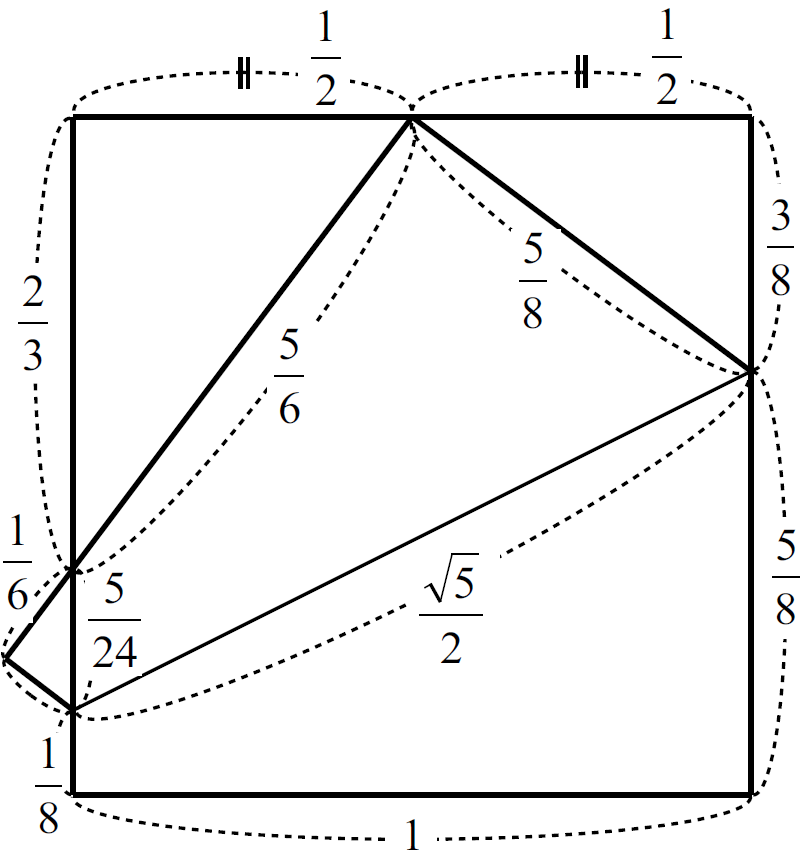
\includegraphics[width=0.45\textwidth]{images/hagovi_izreki/hagov_izrek1_stevilke.png}
    \caption[Prvi Hagov izrek v številkah]{Dolžine daljic po prvem Hagovem izreku. Vzeto iz~\cite[str. 7]{haga2008}.}
    \label{fig:hagov_izrek1_st}
\end{figure}

Izrek lahko tudi posplošimo, če za točko $E$ ne vzamemo razpolovišča, temveč poljubno točko na daljici $AD$. Naj bo $x = |ED|$. Nastale točke označimo kot prej, dolžine nastalih daljic pa z $y_1$ do $y_6$, kot kaže slika~\ref{fig:hagov_izrek1_splosen}.

\begin{figure}[h]
    \centering
    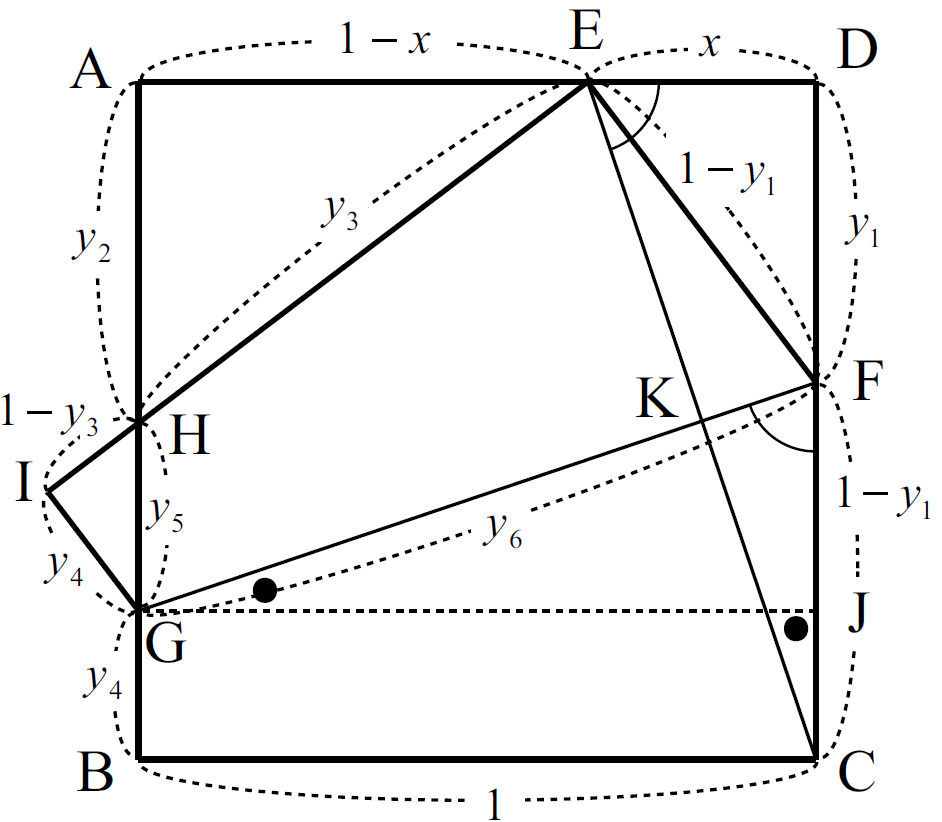
\includegraphics[width=0.55\textwidth]{images/hagovi_izreki/hagov_izrek1_splosen.png}
    \caption[Prvi Hagov izrek v splošnem]{Oznake dolžin iz prvega Hagovega izreka v splošnem. Vzeto iz~\cite[str. 9]{haga2008}.}
    \label{fig:hagov_izrek1_splosen}
\end{figure}

Za vsak $i \in \{1,2,3,4,5,6\}$ poiščimo sedaj vrednost $y_i$ v odvisnosti od $x$. Kot prej najprej opazimo, da imamo zopet tri podobne pravokotne trikotnike. Iz Pitagorovega izreka za pravokotni trikotnik $\triangle EDF$ sledi
$$y_1 = (1-x^2)/2,$$
iz razmerja podobnih pravokotnih trikotnikov $\triangle EDF$ in $\triangle HAE$ pa izračunamo
$$ y_2 = \frac{x(1-x)}{y_1} = \frac{2x}{1+x} \; \text{ in } \; y_3 = \frac{(1-y_1)(1-x)}{y_1} = \frac{1+x^2}{1+x}.$$
Pregib $FG$ je po konstrukciji simetrala daljice $CE$, torej pravokotna nanjo, iz česar sledi, da sta trikotnika $\triangle CKF$ in $\triangle CDE$ podobna in kota $\angle DEC$ in $\angle KFC$ skladna. Zato sta skladna tudi trikotnika $\triangle CDE$ in $\triangle GJF$, torej $|FJ| = x$. Posledično je
$$y_4 = |CJ| = 1 - (y_1 + x) = \frac{(1-x)^2}{2} \; \text{ in } \; y_5 = 1 - y_2 - y_4 = \frac{(1-x)(1+x^2)}{2(1+x)}.$$
Na koncu še s ponovno uporabo Pitagorovega izreka izračunamo
$$ y_6 = \sqrt{|GJ|^2 + |FJ|^2} = \sqrt{1 + x^2}.$$

Splošne vrednosti dolžin $y_i$ mogoče niso najlepše, vendar pri marsikateri izbiri števila $x \in (0,1)$ dobimo lepe številke. Najbolj so zanimiva recipročna števila naravnih števil. Vemo že, da pri izbiri $x = 1/2$ lahko dobimo števila $1/3, 1/6, 1/8$, pri izbiri $x = 1/4$ in $x = 3/4$ dobimo še $2/5$ (in iz tega z razpolovitvijo $1/5$) in $1/7$. Računanje prepuščamo bralcu, se pa na tej točki lahko vprašamo, ali za vsak $n \in \N$ obstaja primeren $x$, da lahko preko neke dolžine $y_i$ ali $1-y_1$ in preko postopkov za konstrukcijo že znanih razmerij konstruiramo dolžino $1/n$. \textcolor{red}{dokaz, da se da??? al pej spusti, če se ti ne da \ldots}

\subsubsection{Drugi Hagov izrek}

\begin{izrek}[Drugi Hagov izrek]
    Zgornjo stranico $AD$ kvadrata $ABCD$ razpolovimo v točki $E$ in opravimo pregib skozi točko $E$ ter oglišče $C$. Točka $D$ se tako preslika v točko $F$ (slika~\ref{fig:hagov_izrek2}). Če stranico $EF$ podaljšamo do leve stranice kvadrata, jo presečišče $G$ razdeli v razmerju $2:1$.
\end{izrek}

\begin{figure}[h]
    \centering
    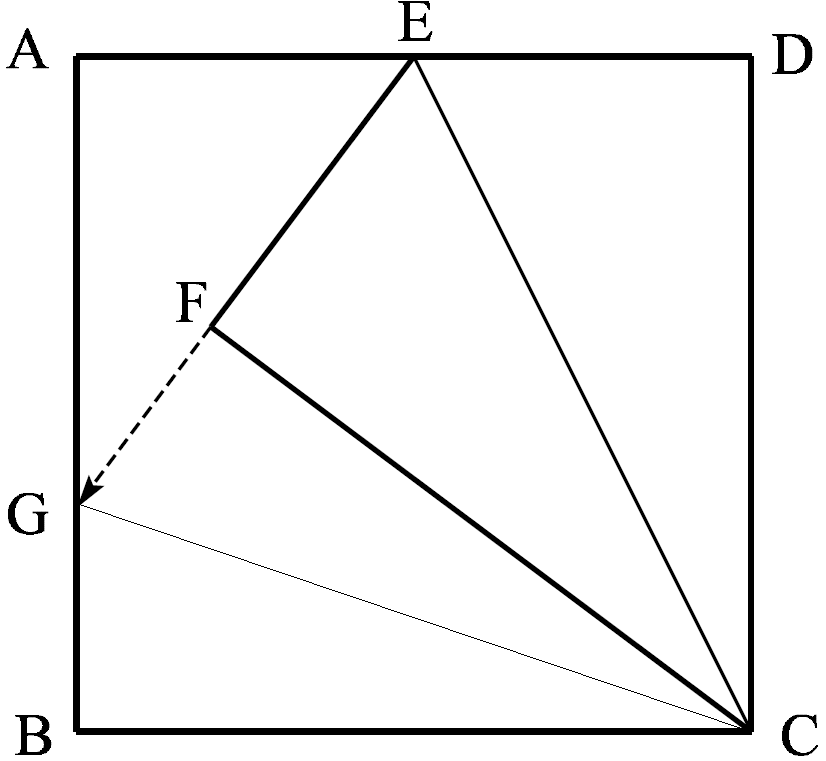
\includegraphics[width=0.4\textwidth]{images/hagovi_izreki/hagov_izrek2.png}
    \caption[Pregib iz drugega Hagovega izreka]{Konstrukcija pregiba iz drugega Hagovega izreka. Vzeto iz~\cite[str. 12]{haga2008}.}
    \label{fig:hagov_izrek2}
\end{figure}

\begin{dokaz}
    Opazimo lahko, da sta trikotnika $\triangle BCG$ in $\triangle FCG$ skladna, saj imata skladni daljšo kateto in hipotenuzo ter pravi kot nasproti hipotenuze. Označimo $x = |GB| = |GF|$. Zapišimo Pitagorov izrek za pravokotni trikotnik $\triangle AGE$:
    $$ \left(x + \frac{1}{2}\right)^2 = (1-x)^2 + \left(\frac{1}{2}\right)^2 \; \text{ in izračunamo } \; x = \frac{1}{3},$$
    torej točka $G$ res deli stranico $AB$ v razmerju $2:1$.
\end{dokaz}

S tem smo zopet dobili način razdelitve daljice na tri enake dele, a tu zanimivih razmerij še ni konec. Poglejmo si še, v kakšen razmerju nam stranice deli točka $F$ in točke, ki jih dobimo s podaljšanjem daljic $FD$ in $FC$ do leve stranice. Označimo nove točke $H, I, J, K$ in $M$, kot kaže slika~\ref{fig:hagov_izrek2_st}.

\begin{figure}[h]
    \centering
    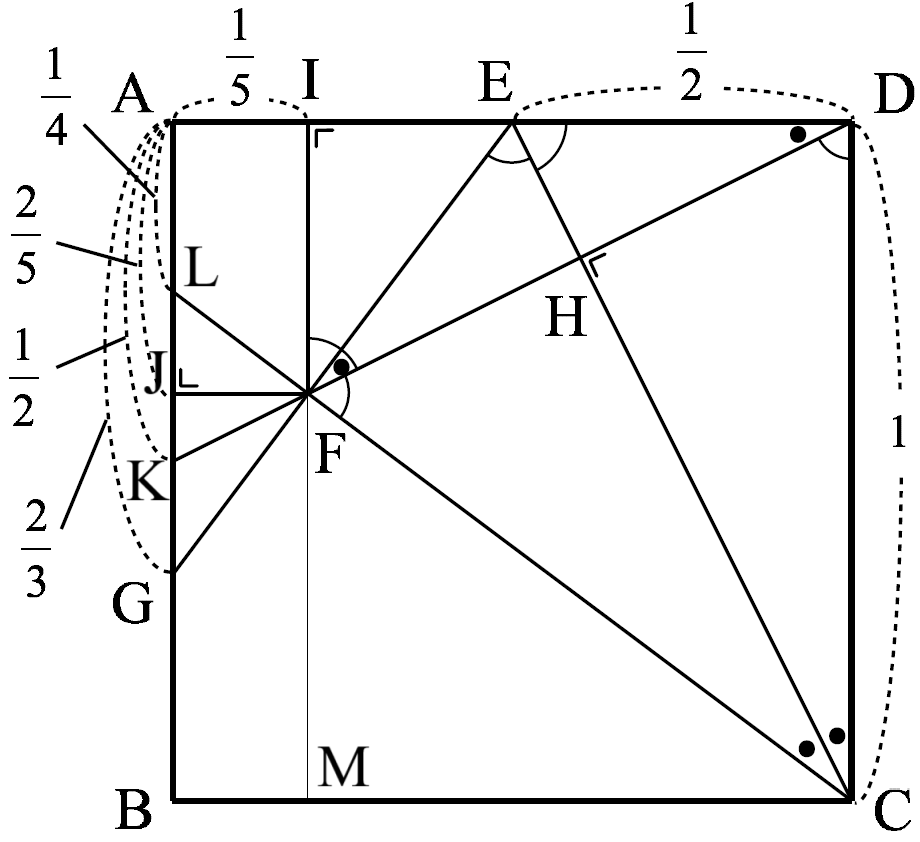
\includegraphics[width=0.45\textwidth]{images/hagovi_izreki/hagov_izrek2_stevilke.png}
    \caption[Drugi Hagov izrek v številkah]{Dolžine daljic po drugem Hagovem izreku. Vzeto in preurejeno iz~\cite[str. 15]{haga2008}.}
    \label{fig:hagov_izrek2_st}
\end{figure}

Po konstrukciji pregiba velja $FD \perp CE$, iz česar dobimo podobne pravokotne trikotnike $\triangle CDE$, $\triangle CFE$, $\triangle DAK$, $\triangle DHE$, $\triangle FHE$, $\triangle DIF$. Prvi trije od naštetih so celo skladni, prav tako je skladen tudi sledeči par. Le trikotnik $\triangle DIF$ nima skladnega para. Iz sledečih razmerij izračunamo
\begin{align*}
    |DH| &= \frac{|DE| \cdot |CD|}{|CE|} = \frac{1}{\sqrt{5}}, \; \text{ torej } \; |DF| = 2|FH| = \frac{2}{\sqrt{5}}, \\
    |DI| &= \frac{|DF| \cdot |CD|}{|CE|} = \frac{4}{5}, \; \text{ torej } \; |AI| = \frac{1}{5}, \\
    |FI| &= \frac{|DI| \cdot |DE|}{|CD|} = \frac{2}{5} \; \text{ in} \\
    |AK| &= |DE| = \frac{1}{2}.
\end{align*}

Iz podobnih trikotnikov $\triangle BCL$ in $\triangle MCF$ sledi še
$$ |BL| = \frac{|BC| \cdot |FM|}{|CM|} = \frac{3}{4}, \; \text{ torej } \; |AL| = |AB| - |BL| = \frac{1}{4}. $$

Torej nam drugi Hagov izrek poleg konstrukcije števil $1/3, 2/3$ poda tudi diretkno konstrukcijo števil $1/5, 2/5, 3/5$ in $4/5$.

\subsubsection{Tretji Hagov izrek}

\begin{izrek}[Tretji Hagov izrek]
    Zgornjo stranico $AD$ kvadrata $ABCD$ razpolovimo v točki $E$ in opravimo pregib, ki točko $E$ položi na desno stranico in hkrati oglišče $C$ na levo stranico (slika~\ref{fig:hagov_izrek3}). Njena slika $H$ levo stranico deli v razmerju $2:1$.
\end{izrek}

\begin{figure}[h]
    \centering
    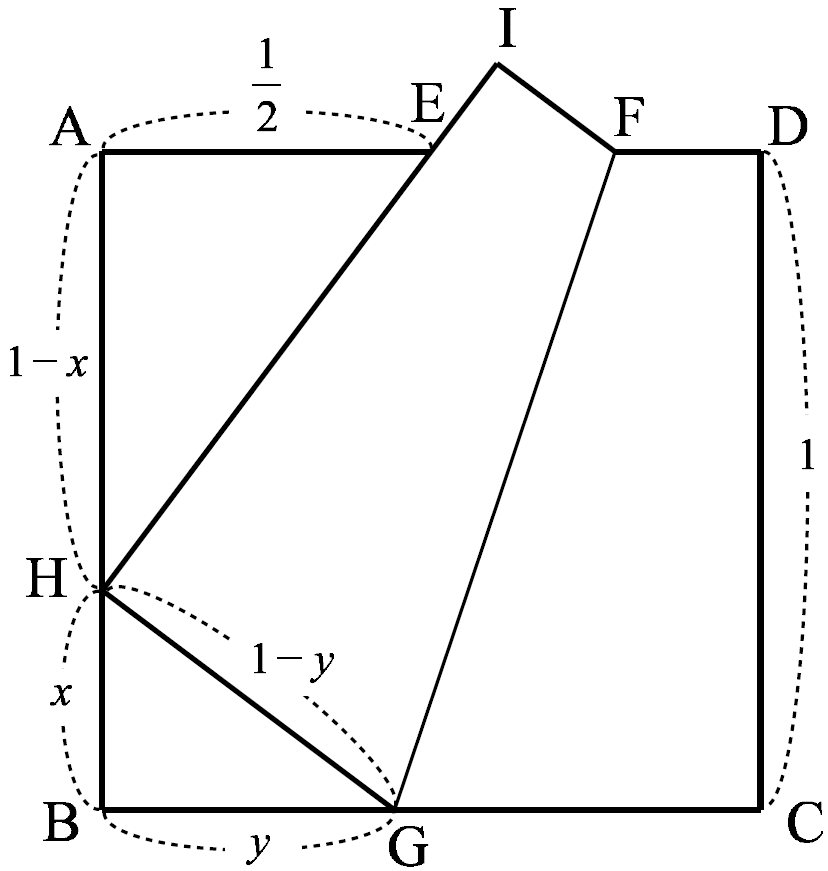
\includegraphics[width=0.45\textwidth]{images/hagovi_izreki/hagov_izrek3.png}
    \caption[Pregib iz tretjega Hagovega izreka]{Konstrukcija pregiba iz tretjega Hagovega izreka. Vzeto iz~\cite[str. 18]{haga2008}.}
    \label{fig:hagov_izrek3}
\end{figure}

\begin{dokaz}
    Označimo še točke $E, F, G,$ in $I$ ter uvedimo $x = |BH|$ in $y = |BG|$, kot kaže slika~\ref{fig:hagov_izrek3}. Zaradi prepogiba je $|GH| = |CG| = 1-y$. Iz Pitagorovega izreka za pravokotni trikotnik $\triangle BGH$ ter razmerja za podobna trikotnika $\triangle BGH$ in $\triangle AHE$ dobimo sistem enačb
    $$ x^2 + y^2 = (1-y)^2 \; \text{ in } \; \frac{1/2}{1-x} = \frac{x}{y}, $$
    iz katerih izračunamo $x = \frac{1}{3}$ in $y = \frac{4}{9}$. Torej točka $H$ res deli stranico $AB$ v razmerju $2:1$.
\end{dokaz}

Kot pri prejšnjih dveh izrekih bi lahko poračunali še preostale dolžine daljic. To za vajo prepuščamo bralcu, ki se lahko o svojih rezultatih prepriča s sliko~\ref{fig:hagov_izrek3_st}.

\begin{figure}[h]
    \centering
    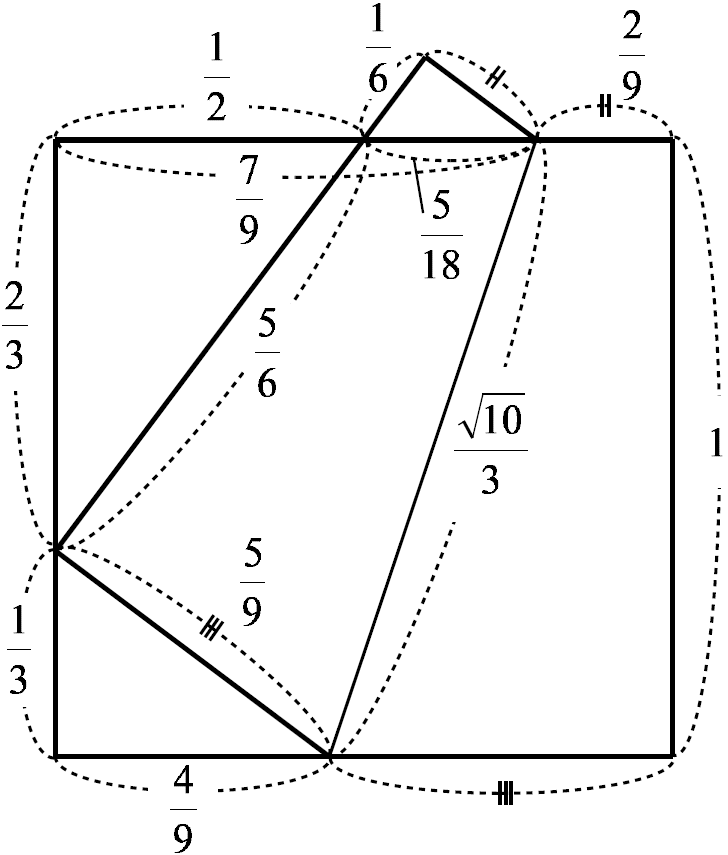
\includegraphics[width=0.45\textwidth]{images/hagovi_izreki/hagov_izrek3_stevilke.png}
    \caption[Tretji Hagov izrek v številkah]{Dolžine daljic po tretjem Hagovem izreku. Vzeto iz~\cite[str. 19]{haga2008}.}
    \label{fig:hagov_izrek3_st}
\end{figure}


\textcolor{red}{Kakšen zaključek teh treh izrekov? Skupno -- vsi trije uporabljajo središče $E$ zgornje stranice $AD$. Prvi izrek nanj položi oglišče $C$, drugi izrek naredi pregib skoznjo in oglišče $C$, tretji pa nanjo položi desno stranico tako, da $C$ leži na levi stranici. Kej skupnega, bi se dalo še kakšen drug pregib blablabla}

\textcolor{red}{Lahko omeniš še srebrne pravokotnike (npr.\ A4 list papirja, stranici sta v razmerju $1 : \sqrt{2}$ in vsakič, ko daš pravokotnik po kratki stranici na pol, dobiš spet srebrn pravokotnik; pač isti princip kot pri zlatem pravokotniku za zlati rez), pa da se da tudi na njih naredit te Hagove izreke. Katere razdelitve dobiš? Na 9, 14, 16 delov itd., poglej vir. Ampak to nej gledajo v~\cite[str.\ 21--32]{haga2008}.}



\subsection{Razdelitev daljice na $n$ enakih delov}

Stranico kvadrata želimo razdeliti na $n$ enakih delov, kjer je $n \in \N$ poljuben. Za $n = 2^t, t \in \N_0$ je to čisto enostavno, saj samo prepolavljamo razdalje med pregibi, dokler ne dosežemo cilja. Če je $n$ sod, vendar ni potenca $2$, torej $n = 2^t(2m + 1)$, kjer sta $t, m \in \N$, stranico najprej razdelimo na $2^t$ delov, nato pa moramo vsakega izmed njih razdeliti na $2m + 1$ (liho število) delov. Izziv tega problema je torej v razdelitvi daljice na liho število delov. Ko bomo zo zmogli, jo bomo znali razdeliti na $n$ delov za vsak $n \in \N$.

V prejšnjem razdelku so nam Hagovi izreki podali razdelitev stranice kvadrata na tri, pet, sedem in devet delov. Vendar iščemo metodo, ki nam stranico razdeli na $n$ delov za splošen lih $n \in \N$. Spomnimo se, da smo en tak postopek že spoznali -- v dokazu izreka~\ref{izr:podpolje} smo za poljuben $a \in \R$ znali konstruirati razdaljo $1/a$, kar bi lahko uporabili za razdelitev neke daljice na $a$ enakih delov -- konstruirano razdaljo $1/a$ bi $a$-krat prenesli naprej. Načinov reševanja tega problema pa se je skozi zadnja desetletja oblikovalo še veliko več; tu si bomo pogledali še \textcolor{red}{koliko?} metode.

\subsubsection*{Metoda križajočih se diagonal}

Metoda nima uradnega prevoda niti uradnega imena, jo pa tako imenuje Robert J.\ Lang v svojem članku~\cite{lang1988}. Njena konstrukcija je prikazana na sliki~\ref{fig:kriz_diag_3}. Najprej kvadrat dvakrat prepognemo na pol -- enkrat po diagonali skozi oglišči $A$ in $C$ in drugič po vertikali. Nato prepognemo po diagonali (skozi oglišče $B$) še desni pokončen pravokotnik. Presečišče obeh diagonal označimo s točko $P$ in naredimo skoznjo prepogib, ki je pravokoten na horizontalno stranico kvadrata.

\begin{figure}[h]
    \centering
    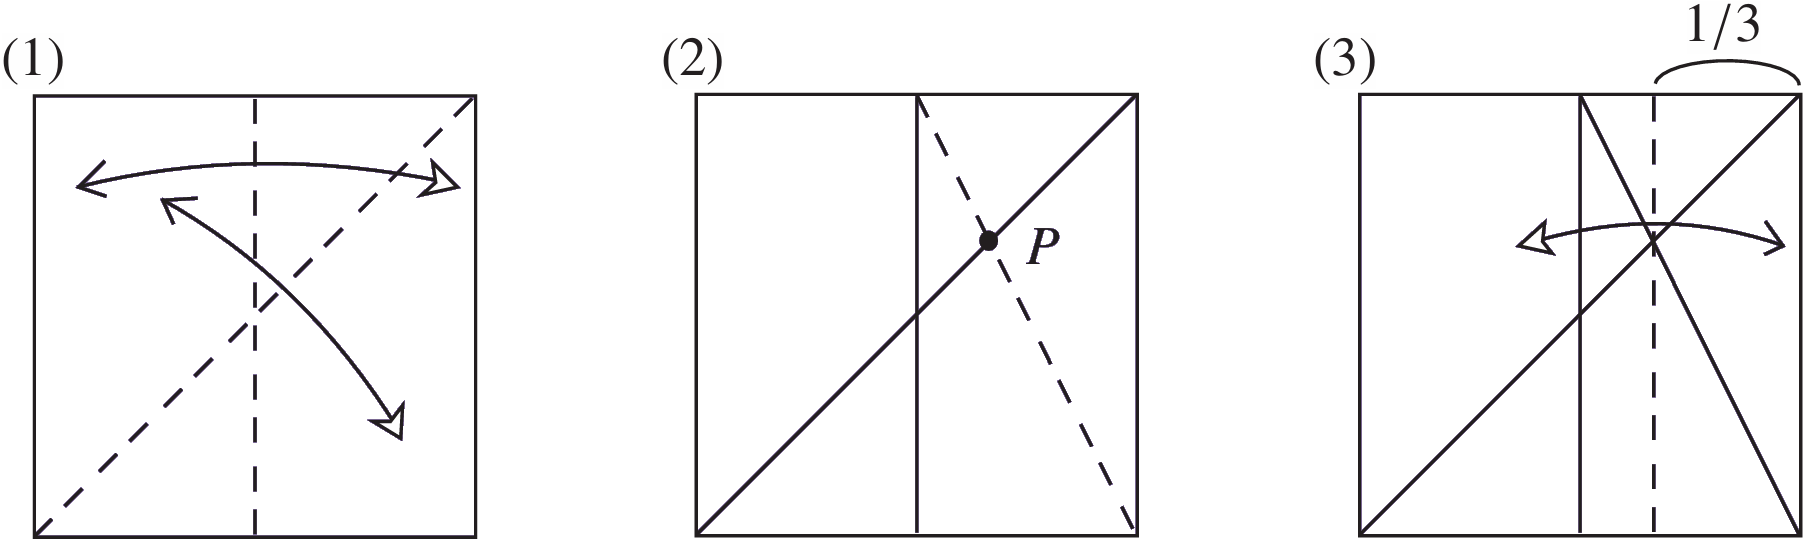
\includegraphics[width=0.9\textwidth]{images/tretjinjenje_stranice1.png}
    \caption[Razdelitev stranice na tri dele]{Konstrukcija po metodi križajoih se diagonal za $n=3$.}
    \label{fig:kriz_diag_3}
\end{figure}

\begin{trditev}
    \label{trd:kriz_diag_3}
    Zadnji pregib iz zgornjega opisa konstrukcije razdeli horizontalno stranico kvadrata v razmerju $2:1$.
\end{trditev}

\begin{dokaz}
    Dokazujemo lahko na več načinov:
    \begin{enumerate}
        \item \textit{Analitičen pristop:} Kvadrat postavimo v evklidsko ravnino tako, da je spodnje levo oglišče kvadrata v koordinatnem izhodišču in spodnje desno v točki $(1, 0)$. Obe diagonali izrazimo z enačbama premic. Glavna diagonala ima enačbo $y = x$, diagonala pravokotnika pa $y = -2x + 2$. Točka $P$ je njuno presečišče in ima tako koordinati $(2/3, 2/3)$.
        \item \textit{Preko podobnih trikotnikov:} Z opisanimi prepogibi v tem kvadratu konstruiramo več trikotnikov. Njihova oglišča označimo tako, kot kaže slika \textcolor{red}{naredi in referiraj sliko, str. 38 v hull2013; ampak predrugači imena oglišč (glej nadaljevanje tega dokaza)}. Iz podobnosti trikotnikov $\triangle AGP$ in $\triangle ABC$ sledi, da je trikotnik $\triangle AGP$ enakokrak. Naj bo dolžina njegovih krakov $x$. Potem je $|AG| = |GP| = x$ in $|GB| = 1 - x$. Iz podobnosti trikotnikov $\triangle EFB$ in $\triangle PGB$ sledi
        \begin{align*}
            \frac{|EF|}{|FB|} &= \frac{|PG|}{|GB|}, \\
            \frac{1}{\frac{1}{2}} &= \frac{x}{1 - x}, \\
            x &= \frac{2}{3}.
        \end{align*}
    \end{enumerate}
\end{dokaz}

Po konstrukciji pregiba, ki zgornjo stranico kvadrata razdeli v razmerju $2:1$, desni pravokotnik (s stranico $DE$) po vertikali prepognemo še na pol. S tem smo stranico kvadrata razdelili na tri enake dele.

Razdelitev stranice kvadrata na štiri dele je očitna -- kvadrat v vertikalni smeri dvakrat prepognemo na pol.

Stranico razdelimo na pet delov na podoben način kot na tri. Naredimo enak pregib po glavni diagonali, nato pa zgornjo stranico razdelimo v razmerju $3:1$ (to znamo storiti). S tem smo na desni strani kvadrata dobili pokončen pravokotnik s horizontalno stranico, dolgo četrt stranice kvadrata. Naslednji pregib je, kot prej, diagonala tega pravokotnika (tista skozi oglišče $B$). Presečišče te in glavne diagonale je točka, ki je od desne stranice oddaljena za $1/5$ (dokaz je analogen tistemu za trditev~\ref{trd:kriz_diag_3}). Naredimo vertikalen pregib skozi točko $P$ in s tem zgornjo stranico kvadrata razdelimo v razmerju $4:1$. Na koncu še levi del te stranice razdelimo na štiri dele. S tem smo celotno stranico razdelili na pet skladnih delov.

Zgornji postopek lahko posplošimo na poljuben $n \in \N$. Kot smo videli v konkretnih primerih za $n = 3, 4$ in $5$, smo si pomagali z vnajprejšnjo razdelitvijo stranice na $n-1$ število enakih delov (kar smo zmogli storiti). Dokaz naslednje trditve bo tako temeljil na indukciji.

\begin{trditev}[Metoda križajočih se diagonal za splošen $n$]
    Naj bo $n \in \N, n > 2$. Kvadrat $ABCD$ s stranico dolžine $1$ prepognemo po diagonali $AC$, potem pa stranico $DC$ s točko $E$ razdelimo v razmerju $(n-2):1$. Naredimo pregib novonastalega pravokotnika skozi točki $B$ in $E$. Presečišče te in glavne diagonale je točka $P$, ki je od desne stranice kvadrata oddaljena za $1/n$.
\end{trditev}

\begin{dokaz}
    Za $n = 1$ in $n = 2$ ni kaj dokazovati -- v prvem primeru pregiba sploh ni, v drugem primeru stranico prepolovimo.

    \textit{Baza indukcije:} Vemo že, da trditev drži za $n = 3, 4, 5$.

    \textit{Indukcijska predpostavka:} Predpostavimo, da znamo stranico razdeliti na $n$ enakih delov.

    \textit{Indukcijski korak:} Dokazujemo, da znamo stranico razdeliti na $n+1$ enakih delov. Po navodilih za konstrukcijo najprej stranico $DC$ s točko $E$ razdelimo v razmerju $(n-1):1$ (kot če bi jo razdelili na $n$ skladnih delov, ampak označimo le zadnji prpogib). To po indukcijski predpostavki znamo storiti. S prepogibom skozi oglišče $B$ in točko $E$ dobimo, kot presečišči obeh diagonal, točko $P$. Potem pa podobno kot pri dokazu trditve~\ref{trd:kriz_diag_3} dokažimo, da leži točka $P$ na želeni razdalji od desne stranice kvadrata:
    \begin{enumerate}
        \item \textit{Analitičen pristop:} Naj bo oglišče $A$ koordinatno izhodišče in oglišče $B$ točka $(1, 0)$. Premica, ki je nosilka diagonale $AC$, ima tako enačbo $y = x$, nosilka diagonale $CE$ pa $y = -nx + n$. Točka $P$ je njuno presečišče in ima tako koordinate $(n/(n+1), n/(n+1))$. Torej je od desne stranice kvadrata res oddaljena za $1/(n+1)$.
        \item \textit{Preko podobnih trikotnikov:} Označimo oglišča trikotnikov, kot kaže slika \textcolor{red}{SLIKA plus REFERENCA}. Trikotnik $\triangle AGP$ je enakokrak in njegova kraka označimo z $x$. Iz razmerij dolžin stranic podobnih trikotnikov $\triangle EFB$ in $\triangle PGB$ sledi
        $$ \frac{|EF|}{|FB|} = \frac{|PG|}{|GB|} \Rightarrow \frac{1}{\frac{1}{n}} = \frac{x}{1 - x} \Rightarrow n - nx = x \Rightarrow x = \frac{n}{n+1}. $$
        Točka $P$ je od desne stranice kvadrata res oddaljena za $x - 1 = 1/(n + 1)$.
    \end{enumerate}

\end{dokaz}

\begin{posledica}
    Poljubno daljico znamo razdeliti na $n$ skladnih delov za vsak $n \in \N$.
\end{posledica}

\begin{dokaz}
    Vzemimo neko daljico poljubne dolžine. Ker znamo konstruirati pravokotnice skozi točke in prenašati razdalje, lahko konstruiramo kvadrat, katereda zgornja stranica dana daljica \textcolor{red}{(spet kakšna slikca več korakov)}. Po zgornji trditvi jo znamo razdeliti v razmerju $(n-1) : 1$ za vsak $n \in \N$. Potem moramo njen daljši del razdeliti na $n-1$ skladnih delov. To storimo na enak način kot prej -- konstruiramo manjši kvadrat s to novo stranico in ponovimo postopek. Ustavimo se, ko na nekem koraku stranico kvadrata razdelimo v ramerju $1:1$. Takrat bo zgornja stranica oz. dana daljica razdeljena na $n$ skladnih delov.
\end{dokaz}

\subsubsection*{Metoda2}

\subsubsection*{Metoda3}

\subsubsection*{Metoda4}

\textcolor{red}{Več metod (vsaj tri?), Hull2013 (str.\ 36--40).}

\textcolor{red}{Do zdaj smo imeli metode z razdelitvijo preko prepogibanja kvadratnega lista papirja. Za razdelitev preko pravokotnika pa glej~\cite[str.\ 107--134].}

\subsection{$X$-pregibi}

\textcolor{red}{Glej~\cite[str.\ 33--44]{haga2008}}


\subsection{Reševanje nerešljivih starogrških problemov}
\label{podpogl:starogrskiproblemi}

Z evklidskimi konstrukcijami se je seveda pojavilo konstruktibilnih ugank -- vprašanj, ali je specifično število konstruktibilno (in na kakšnen način) ali ne. Zelo znani so trije t.\ i.\ ``starogrški' problemi, ki so matematike bremenili več kot tisočletje, začenši s časom Evklida (300 pr.\ Kr.), končno pa sta nanje dokončno odgovorila Niels Henrik Abel (1802--1829) in Evariste Galois (1811--1832) v začetku 19.\ stoletja. Gre za sledeče tri probleme:
\begin{itemize}
    \item \textbf{Podvojitev kocke} Imejmo že konstruktibilno kocko. Konstruiraj novo kocko, ki ima dvakrat večji volumen od prve (problem se poenostavi na iskanje konstrukcije števila $\sqrt[3]{2}$).
    \item \textbf{Trisekcija kota} Dan je poljuben konstruktibilen kot. Konstruiraj kot, ki prvega deli na tri skladne dele.
    \item \textbf{Kvadratura kroga} Za dan konstruktibilen krog konstruiraj kvadrat, ki ima enako ploščino kot dani krog (problem se poenostavi na konstrukcije števila $\sqrt{\pi}$).
\end{itemize}

Z znanjem, ki sta ga znanosti posredovala Abel in Galois, se da pokazati, da ti trije problemi z evklidskim orodjem niso rešljivi. V nalogi smo do sedaj že večkrat omenili, da pa obstajajo origami konstrukcije (celo več metod za isti problem!), ki nam konstruirajo kubični koren origami števila ter razdelijo kot na tri skladne dele. Žal pa je to še vedno premalo za konstrukcija števila $\sqrt{\pi}$.

\subsubsection{Podvojitev kocke}
\label{podpogl:podvojitev_kocke}

Po legendi iz grške mitologije je bog Apolon po oraklju prebivalcem svojega rojstnega otoka Delosa sporočil, da mu morajo, če se želijo znebiti smrtonosne kuge, zgraditi nov oltar v obliki kocke, ki je enak prejšnjemu, le da mora biti dvakrat večji po prostornini. Torej je bilo potrebno konstruirati kocko s stranico, ki je za faktor $\sqrt[3][2]$ večja od stranice originalne kocke. Po drugi legendi pa naj bi Platon izjavil, da je ta problem, ki so ga prejeli na njegovi Akademiji v Atenah, poslan od bogov samih z namenom osramotiti Grke zaradi njihovega zanemarjanja in prezira do matematike (ker z evklidskim orodjem niso znali konstruirati poljubnih dolžin).

Problem najprej poglejmo skozi algebrsko okno. Če je stranica kocke dolga 1, je stranica podvojene kocke dolga $\sqrt[3]{2}$. Ker je obseg $\Q(\sqrt[3]{2})$ vektorski prostor razsežnosti $3$ nad obsegom $\Q$ (enačba $ x^3 - 2 = 0 $ nima racionalne rešitve), podvojitev kocke po izreku~\ref{izr:evkl_konstr} ni mogoča~\cite[str. 78]{jerman1998}.

\textcolor{red}{Grki so to rešili s presečiščem dveh parabol -- glej~\cite[str.\ 5--6]{videla1997}, kar je zelo podobno oni iz~\cite[str.\ 156]{geometricconstructions} (za poljuben $k$!). Tukej daj samo slikco 10.7 in napiši, da za dokaz gledajo tistega pri konstrukciji preko Belochinega kvadrata (v razdelku~\ref{podpogl:beloch_kvadrat_koren}). No, lahko pa tukaj dokažeš in v poglavju z enačbami referiraš, da je možno s kvadratom konstruirati in je to isto kot tle. Sam da tukaj ne zarišeš kvadrat. Ker ga v resnici ni treba. Če se tko odločiš, pol spremeni tisto podpoglavje v samo omembo.}

\subsubsection*{Messerjeva konstrukcija}

Peter Messer je v~\cite{messer1986} podal naslednjo preprosto konstrukcijo, ki ne konstruira števila $\sqrt[3]{2}$ kot razdaljo, temveč kot razmerje: kvadrat po horizontali razdelimo na tri dele (to sedaj že znamo storiti) ter točki $p_1$ in $p_2$ s prepogibom položimo na premici $L_1$ in $L_2$, kot kaže slika~\ref{fig:messer} (levo).
\begin{figure}[h]
    \centering
    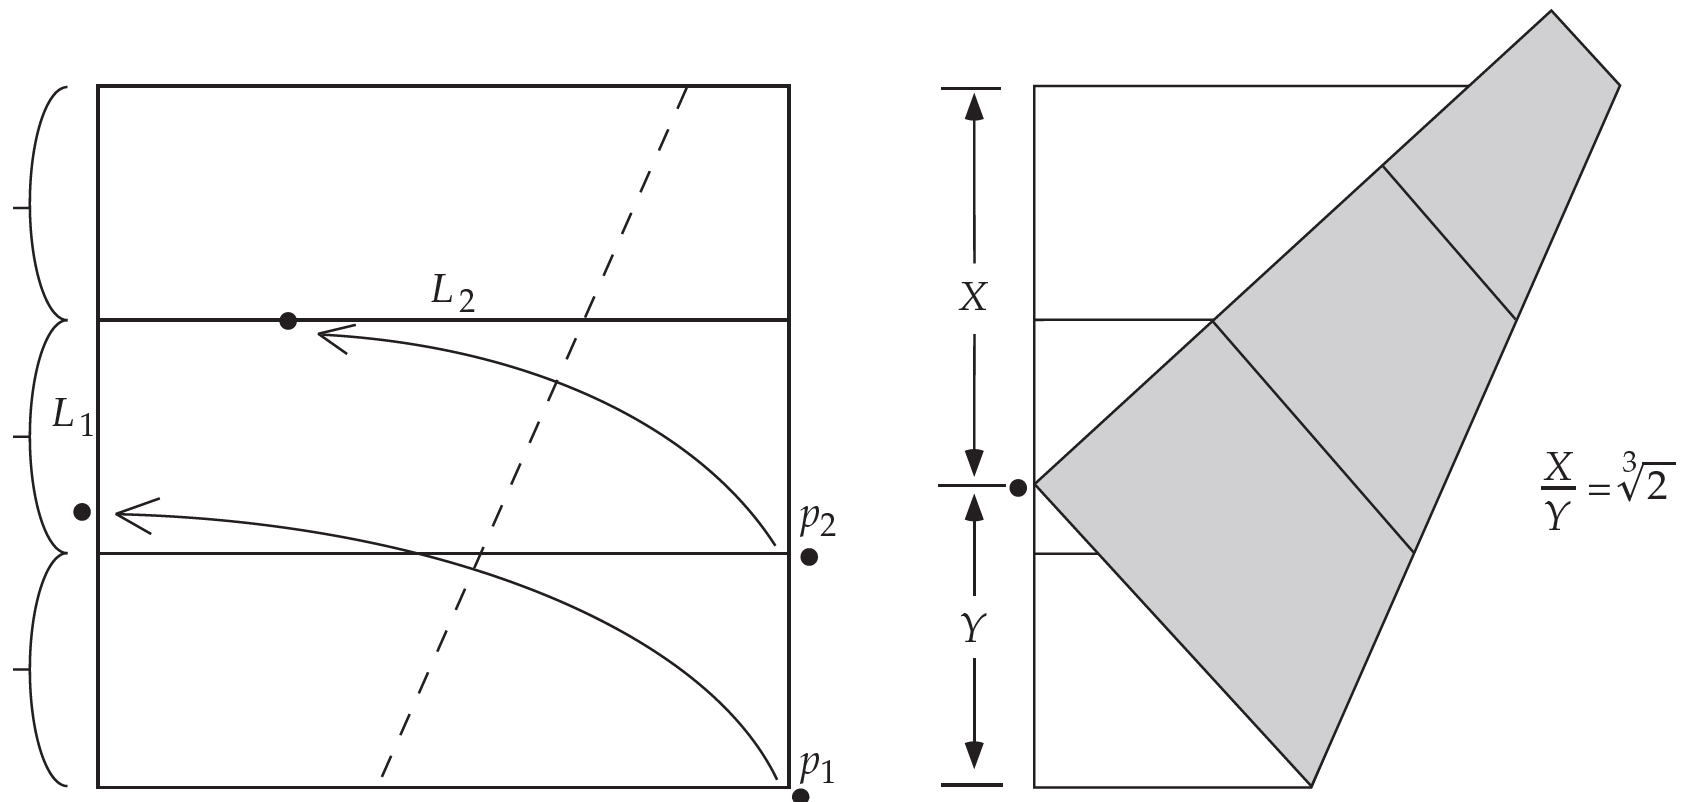
\includegraphics[width=0.68\textwidth]{images/starogr_problemi/messer1.png}
    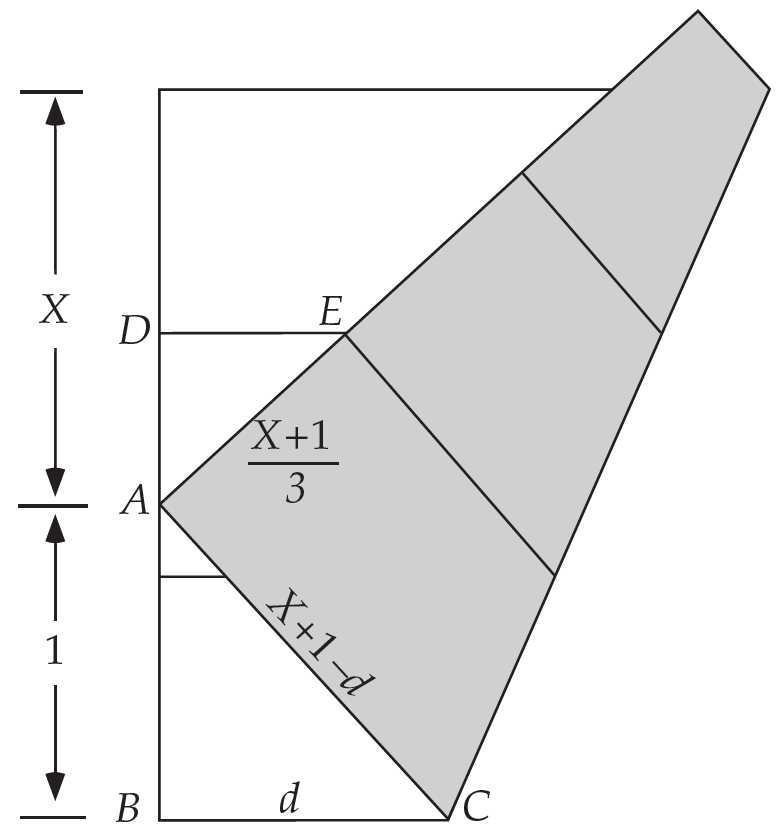
\includegraphics[width=0.3\textwidth]{images/starogr_problemi/messer2.png}
    \caption[Messerjeva konstrukcija]{Messerjeva konstrukcija razmerja $\sqrt[3]{2}$. Vzeto iz~\cite[str.\ 67--68]{hull2013}.}
    \label{fig:messer}
\end{figure}
\begin{trditev}
    Slika točke $p_1$ deli levo stranico kvadrata v razmerju $\sqrt[3]{2}$.
\end{trditev}
\begin{dokaz}
    Vpeljimo oznake $X, Y, A, B, C, D, E$ ter $d = |BC|$, kot kaže slika~\ref{fig:messer}. Dokazati moramo $X/Y = \sqrt[3]{2}$, za lažje računanje pa brez škode privzemimo $Y=1$. Stranica kvadrata je tako dolga $X+1$, zato je $|AC| = X+1-d$ in $|AE| = (X+1)/3$.

    Opazimo podobna pravokotnika $\triangle ABC$ in $\triangle ADE$. Iz trikotnika $\triangle ABC$ s pomočjo Pitagorovega izreka izrazimo $d = (X^2+2X)/(2X+2)$, preko leve stranice pa še $|AD| = X - (X+1)/3 = (2X-1)/3$. Iz podobnosti omenjenih trikotnikov izrazimo razmerje katete in hipotenuze z enačbo $|BC|/|AC| = |AD|/|AE|$. Ko vstavimo noter vse vrednosti, odvisne od $X$, dobimo enačbo
    $$ \frac{X^2 + 2X}{X^2 + 2X + 2} = \frac{2X - 1}{X + 1},$$
    ki se nam poenostavi prav v $X^3 = 2$. Torej je $X = \sqrt[3]{2}$.
\end{dokaz}

Še ena konstrukcija $\sqrt[3]{a/b}$ je v~\cite[str.\ 366--367]{geret1995}.



\subsubsection{Trisekcija kota}
\label{podpogl:trisekcija}

Kot $90^\circ$ znamo tretjiniti z neoznačenim ravnilom in šestilom, saj znamo konstruirati kot $30^\circ$. Težava je, da ne obstaja konstrukcija, s katero na tri skladne kote razdelimo \emph{poljuben} kot. V~\cite[str.\ 77--78]{jerman1998} je dokaz o nezmožnosti trisekcije kota $60^\circ$. Avtor se pri tem sklicuje na izrek~\ref{izr:evkl_konstr} in opombo~\ref{op:razseznost_obsega_evkl} iz razdelka~\ref{podpogl:evkl_konstruktibilnost}.

% SPODNJI DOKAZ JE PREPISAN IZ VIRA IN SAMO CITIRAN V POGLAVJU 2.3

% Algebraični dokaz, da z evklidskim orodjem ne moremo tretjiniti poljubnega kota -- dokažimo za kot $60°$. (iz~\cite[str.\ 77--78]{jerman1998})

% Kot $60°$ znamo narisati. Če bi ga znali razdeliti na tri enake dele, bi potemtake znali narisati tudi kot $20°$, s tem pa (ker znamo risati pravokotnice) tudi $\cos 20°$ \textcolor{red}{slika z enotsko krožnico}. Pokažimo, da to ne gre.

% Izračunajmo minimalni polinom števila $\cos 20°$. Ker je
% $$ \frac{1}{2} = \cos 60° = \cos(3 \cdot 20°) = 4 \cos^3 20° - 3 \cos 20°, $$
% ima polinom $ p(x) = 8 x^3 - 6x - 1 $ ničlo $ \cos 20°$. Minimalni polinom števila $ \cos 20°$ deli polinom $p$. Če polinom $p$ razpade na produkt dveh polinomov s koeficienti v $\Q$, je eden od polinomov zagotovo linearen. To pa bi pomenilo, da ima polinom $p$ vsaj eno racionalno ničlo. Edini kandidatki za racionalne ničle polinoma $p$ so števila iz množice
% $$ \{\pm 1, \pm \frac{1}{2}, \pm \frac{1}{4}, \pm \frac{1}{8} \}. $$4Nobeno od teh števil ni ničla polinoma $p$, zato se $p$ ne da razcepiti na produkt dveh polinomov z racionalnimi koeficienti. Minimalni polinom števila $ \cos 20°$ je torej enaka
% $$ m(x) = \frac{1}{8} p(x) = x^3 - \frac{3}{4} x - \frac{1}{8}. $$
% Tako je razsežnost prostora $\Q(\cos 20°)$  nad obsegom $\Q$ enaka $3$ in števila $ \cos 20° $ se ne da narisati le z ravnilom in šestilom.

% Zato trisekcija kota v splošnem ni mogoča.

\textcolor{red}{Grki so to reševali z uporabo hiperbole -- glej~\cite[str.\ 9]{videla1997}. V tem članku so opisane vse točke, ki se jih da kosntruirati s stožnicami (in gre za ista števila kot z origamijem?) dobimo množico, zaprto za korenjenje in tretji koren \ldots}

Z origamijem pa obstaja celo več načinov, kako poljuben kot razdeliti na tri skladne dele. \textcolor{red}{če vsi tevi postopki vključujejo Belochin pregib, to napiši tukej in zbriši pri vsakem postopku. Pač bi moral vsak postopek to met vključeno ja, čene ne bi blo logično.}

\subsubsection*{Abejeva metoda}

Sledeča metoda ima ime po japonskemu matematiku Hisashiju Abeju, ki jo je zapisal v svojem članku leta 1980. Postopek vključuje Belochin pregib, torej se ga ne da izvesti z evklidskim orodjem, edina pomankljivost metode pa je, da deluje le za ostre kote. Postopek je sledeč:

\begin{enumerate}
    \item Na kvadratnem listu papirja konstruiramo poljuben kot $\theta$, ki ima vrh v spodnjem desnem vogalu in en krak na spodnji stranici. Nato konstruiramo še dva horizontalna in ekvidistančna pregiba na dnu papirja (slika~\ref{fig:abe_1} levo).
    \item Točko $p_1$ prepognemo na spodnji horizontalen pregib, označen $L_1$, točko $p_2$ pa na poševen krak kota, označen z $L_2$ (slika~\ref{fig:abe_1} na sredi).
    \item Preden pregib razgrnemo, podaljšamo pregib $L_1$ do konca in nov pregib označimo z $L_3$ (slika~\ref{fig:abe_1} desno).
    \item Papir razgrnemo in tokrat v spodnji levi kot podaljšamo pregib $L_3$.
\end{enumerate}

\opomba{V $3$.\ koraku opravimo pregib še preden smo razgrnili prvega. To je za nas načeloma prepovedana poteza, vendar bi se dalo $L_3$ konstruirati tudi po klasični poti z enkratnimi prepogibi -- označili bi sliko točke, ki leži hkrati na $L_1$ in levi stranici kvadrata, ter točko v pregibu iz $2$.\ koraka, ki leži na $L_1$ in skozinju naredili pregib $L_3$ -- zato zaradi lažje izvedbe brez škode dopustimo tak postopek.}

\begin{figure}[h]
    \centering
    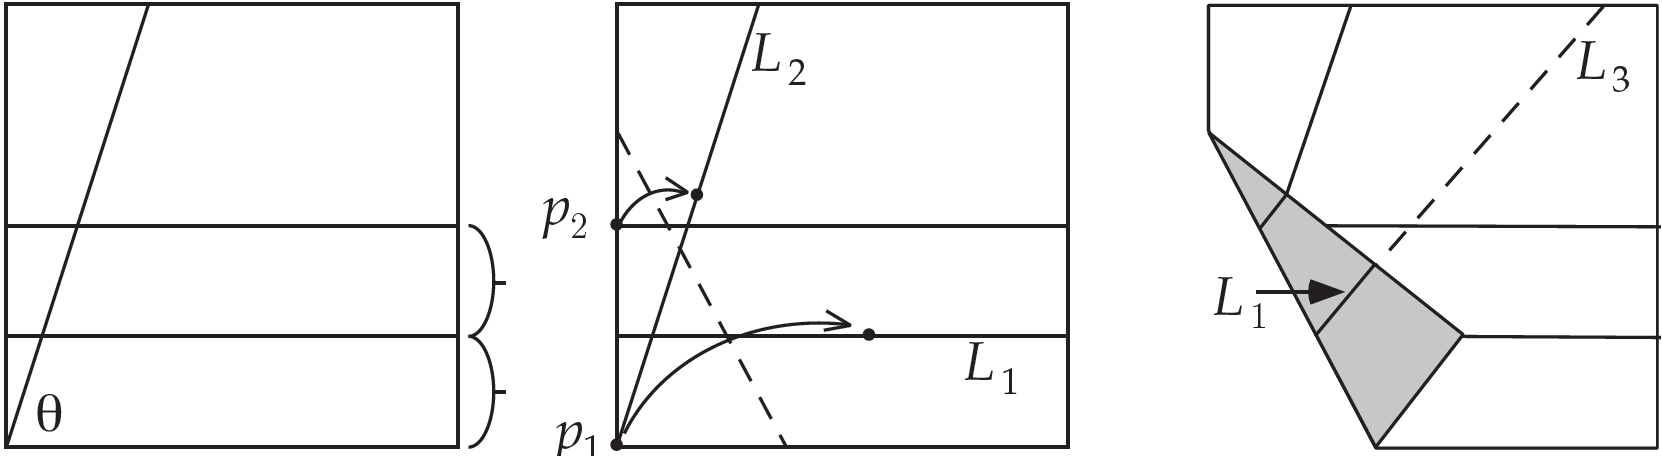
\includegraphics[width=0.95\textwidth]{images/starogr_problemi/abe_nastavek1.png}
    \caption[Abejeva metoda ($1$.\ del)]{Trisekcija kota po Abejevi metodi. Vzeto iz~\cite[str.\ 64]{hull2013}.}
    \label{fig:abe_1}
\end{figure}

\begin{trditev}
    Pregib $L_3$ poteka skozi točko $p_1$. Kot s krakoma $L_2$ in $L_3$ ter vrhom v točki $p_1$ je velik $\theta/3$.
\end{trditev}
\begin{posledica}
    Ko spodnji rob kvadrata prepognemo na pregib $L_3$, razdelimo kot $\theta$ na tri skladne kote.
\end{posledica}

\begin{dokaz}
    Posledica logično sledi, zato dokazujemo le trditev. Označimo z $x$ točko, ki leži na presečišču pregiba $L_1$ in pregiba iz $2$.\ koraka Abejeve metode. Z $A, B$, in $C$ označimo še slike točk z leve stranice kvadrata, kot kaže slika~\ref{fig:abe_2}.
    \begin{figure}[h]
        \centering
        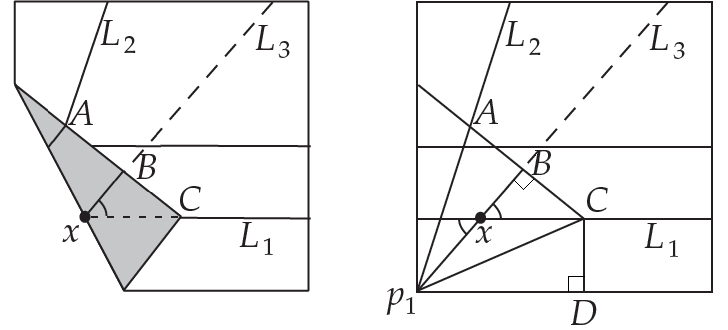
\includegraphics[width=0.7\textwidth]{images/starogr_problemi/abe_trisekcija.png}
        \caption[Abejeva metoda ($2$.\ del)]{Dokazovanje Abejeve metode. Vzeto in predelano iz~\cite[str.\ 65]{hull2013}.}
        \label{fig:abe_2}
    \end{figure}
    Ker je točka $C$ slika točke $p_1$ in $x$ leži na $L_1$, daljica $xC$ leži na $L_1$. Po konstrukciji daljica $xB$ leži na $L_3$, zato sta kota ob $x$, ko papir razgrnemo, skladna. Zaradi sovršnosti kotov daljica $p_1x$ leži na $L_3$, s čimer je prvi del trditve dokazan.
    
    Na razgrnjenem papirju zarišemo (ali prepognemo) še nekaj daljic (slika~\ref{fig:abe_2} desno). Ker velja $|AB| = |BC| = |CD|$ in imata pravokotna trikotnika $\triangle p_1AB$ in $\triangle p_1BC$ skupno še drugo kateto, trikotnika $\triangle p_1BC$ in $\triangle p_1CD$ pa skupno hipotenuzo, so vsi trije trikotniki skladni z enakim kotom v točki $p_1$, torej nam pregiba skozi daljici $p_1B$ (kar je ravno $L_3$) in $p_1C$ kot $\theta$ razdelijo na tri skladne kote.
\end{dokaz}

Ker ta postopek deluje le za ostre kote, si poglejmo naslednjo metodo, ki jo lahko uporabljamo tako za ostre kot tudi tope kote.

\subsubsection*{Justinova metoda}

Avtor Justin:
\begin{itemize}
    \item \cite[str.\ 34]{lang2013}
\end{itemize}

\subsubsection*{Še nekaj metod brez znanih avtorjev}

Gleason's trisection~\cite{gleason1988}, ma mogoče ne teve

\cite[str.\ 154--155]{geometricconstructions}
\cite[str.\ 158 nal. 10.14]{geometricconstructions}
\newpage
\section{Reševanje nerešljivih starogrških problemov}
\label{pogl:starogrskiproblemi}

Z evklidskimi konstrukcijami se je seveda pojavilo konstruktibilnih ugank -- vprašanj, ali sta specifična razdalja oz.\ kot konstruktibilna (in na kakšnen način) ali ne. Stremeli so k iskanju konstrukcij z evklidskim orodjem in če so kakšen problem uspeli rešiti le z neoznačenim ravnilom in šestilom, so te konstrukcije obravnavali kot ``boljše rešitve''~\cite[str. 36]{royster2002}. Grki pa seveda niso delali le s tem orodjem, ampak so se na primer poslužili tudi označenega ravnila\footnote{Martin v trditvi $10.4$ in preko poglavja $9$ v~\cite{geometricconstructions} dokaže, da so origami števila natanko tista množica števil, ki se jih da konstruirati z ravnilom, ki ima na robu dve oznaki.}, s katerim so lahko rešili probleme, ki jih sicer niso mogli. Zelo znani so trije t.~i.\ ``starogrški' problemi, ki so matematike bremenili več kot tisočletje, začenši s časom Evklida (300 pr.\ Kr.), nanje pa sta dokončno odgovorila šele Niels Henrik Abel (1802--1829) in Evariste Galois (1811--1832) v začetku 19.\ stoletja. Gre za sledeče tri probleme:
\begin{itemize}
    \item \textbf{Podvojitev kocke} Imejmo že konstruktibilno kocko. Konstruiraj novo kocko, ki ima dvakrat večji volumen od prve (problem se poenostavi na iskanje konstrukcije števila $\sqrt[3]{2}$).
    \item \textbf{Trisekcija kota} Dan je poljuben konstruktibilen kot. Konstruiraj kot, ki prvega deli na tri skladne dele.
    \item \textbf{Kvadratura kroga} Za dan konstruktibilen krog konstruiraj kvadrat, ki ima enako ploščino kot dani krog (problem se poenostavi na konstrukcije števila $\sqrt{\pi}$).
\end{itemize}

Z znanjem, ki sta ga znanosti posredovala Abel in Galois, se da pokazati, da ti trije problemi z evklidskim orodjem niso rešljivi. V knjigi o starogrški matematiki od Talesa do Evklida~\cite[str.\ 218--270]{heath1921} je zbrano veliko zamisli in konstrukcij grških matematikov, ki so se ukvarjali s temi tremi problemi in evklidsko orodje ne zadostuje za nobeno od najdenih rešitev.

V nalogi smo do sedaj že večkrat omenili, da pa obstajajo origami konstrukcije (celo več metod za isti problem!), ki nam konstruirajo kubični koren origami števila ter razdelijo kot na tri skladne dele. Vse metode, ki bodo sedaj naštete, zahtevajo uporabo Belochinega pregiba (operacije~\ref{op:O7}), kar je logično, saj so vse ostale origami operacije dovolj za vse evklidske konstrukcije. Žal pa tudi tu ostajamo nemočni glede konstrukcije števila $\sqrt{\pi}$, saj je transcedentno in ga ne moremo konstruirati z nobeno od osnovnih operacij vključno s kvadratnim in kubičnim korenjenjem.

\subsection*{Konstrukcija števila $\sqrt{r}$}

Preden si pogledamo konstrukcijo kubičnega korena, vzemimo origami število $r \in \OR$ in konstruirajmo njegov kvadratni koren (postopek je vzet iz~\cite[str.\ 58]{hull2013}).

Imejmo točko $A (0, 1) $ in premico $y = -1$. Na ordinatni osi označimo točko $B (0, -r/4)$ in z operacijo~\ref{op:O6} skoznjo naredimo pregib, ki točko $A$ položi na premico $y = -1$. Njena zrcalna slika je $A' (t, 0) $ za nek $t \in \R$ (slika~\ref{fig:konstrukcija_korena}).

\begin{figure}[h]
    \centering
    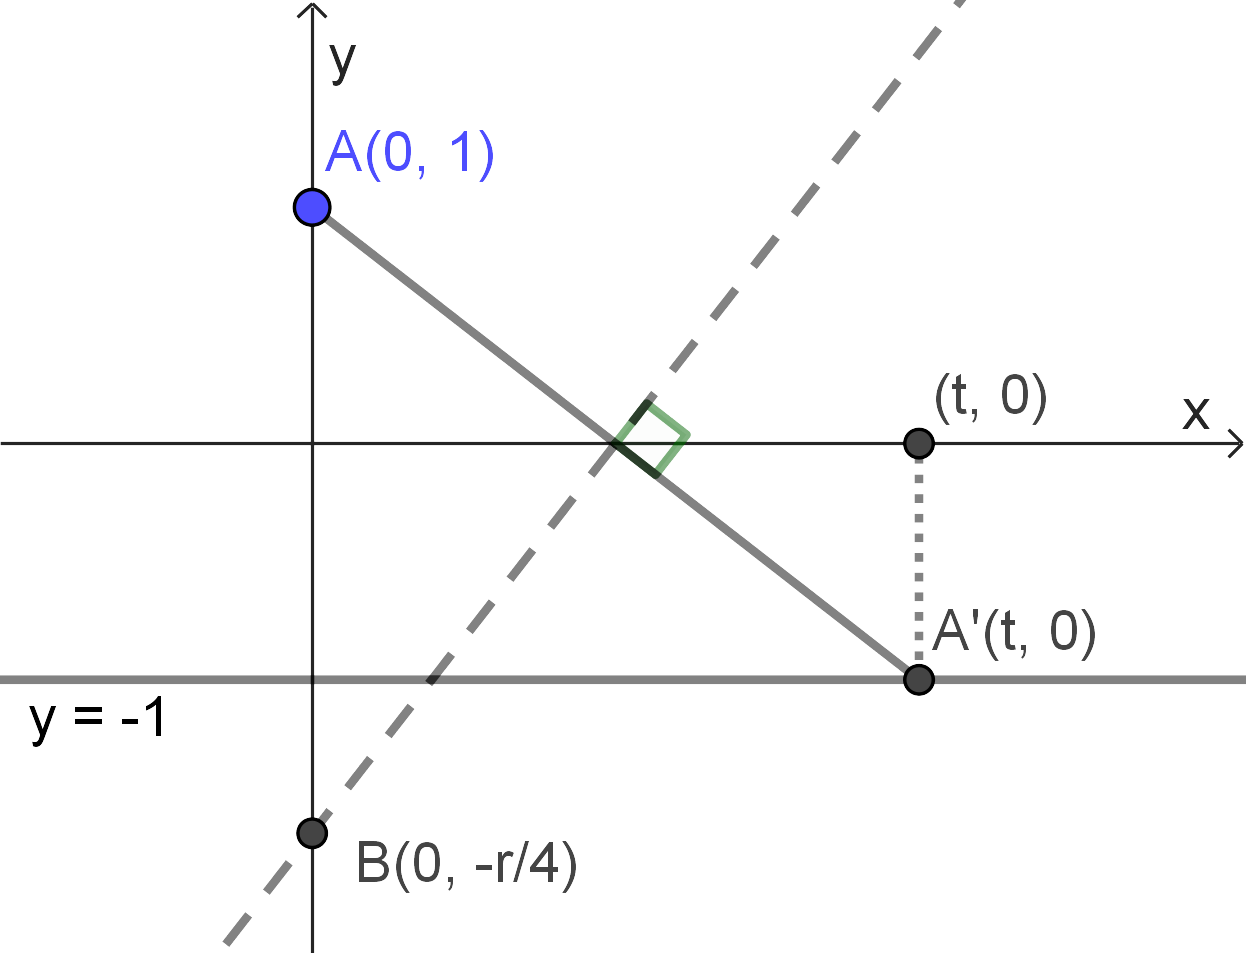
\includegraphics[width=0.5\textwidth]{images/kvadratni_koren.png}
    \caption[Konstrukcija korena]{Konstrukcija števila $\sqrt{r}$ za poljuben $r \in \Q^{+}$.}
    \label{fig:konstrukcija_korena}
\end{figure}

Pregib po konstrukciji poteka skozi točko $B$ in razpolovišče daljice $AA'$, torej je njegov koeficient $k_B = \frac{r}{2t}$ (izpeljavo prepuščamo bralcu). Ker je pregib simetrala daljice $AA'$, njena nosilka pa ima koeficient $k_A = - \frac{2}{t}$, dobimo
\begin{align*}
    k_B &= - \frac{1}{k_A},\\
    \frac{r}{2t} &= \frac{t}{2},\\
    r &= t^2 \text{ oz. } t = \sqrt{r}.
\end{align*}
Na koncu le še prepognemo pravokotnico na abscisno os skozi točko $A'$ in tako dobimo točko $(\sqrt{r}, 0)$. Torej smo konstruirali število $\sqrt{r}$ za poljuben $r \in $.

\subsection{Podvojitev kocke}
\label{podpogl:podvojitev_kocke}

Po legendi iz grške mitologije je bog Apolon po oraklju prebivalcem svojega rojstnega otoka Delosa sporočil, da mu morajo, če se želijo znebiti smrtonosne kuge, zgraditi nov oltar v obliki kocke, ki je enak prejšnjemu, le da mora biti dvakrat večji po prostornini. Torej je bilo potrebno konstruirati kocko s stranico, ki je za faktor $\sqrt[3]{2}$ večja od stranice originalne kocke. Po drugi legendi pa naj bi Platon izjavil, da je ta problem, ki so ga prejeli na njegovi Akademiji v Atenah, poslan od bogov samih z namenom osramotiti Grke zaradi njihovega zanemarjanja in prezira do matematike (ker z evklidskim orodjem niso znali konstruirati poljubnih dolžin)~\cite[str.\ 29]{geometricconstructions}.

Ne vemo, ali so bili Grki prepričani, da se problema z neoznačenim ravnilom in šestilom ne da rešiti. Vsekako pa jim je manjkalo algebrsko znanje iz razdelka~\ref{podpogl:evkl_konstruktibilnost}.

\subsubsection*{Starogrška rešitev preko presečišča dveh parabol}

Grki so problem vseeno uspeli rešiti, čeprav po drugi poti; uporabili so še eno močno matematično orodje -- stožnice. Videla v~\cite{videla1997} dokaže izrek, ki je identičen izreku~\ref{izr:orig_razp_polje} (ki govori, katera števila so origami števila), le da namesto origamija uporabi stožnice. V bistvu s tem dokaže, da so origami konstrukcije ekvivalentne konstrukcijam s stožnicami!

V istem viru Videla tudi navaja konstrukcijo s parabolami, ki za dano dolžino $a$ podajo dolžino $c$, za katero velja $c^3 = a$. Njen avtor je Menehmo (prb.\ 350 pr.\ Kr.), ki je bil tutor samemu Aleksandru Velikemu. Vzel je sledeči paraboli (slika~\ref{fig:videla}):
\begin{itemize}
    \item $\mathcal{P}_1: y = x^2$ z goriščem v točki $(0, \frac{1}{4})$ in premico vodnico $y = - \frac{1}{4}$ in
    \item $\mathcal{P}_1: x = \frac{y^2}{a}$ z goriščem v točki $(\frac{a}{4}, 0)$ in premico vodnico $x = - \frac{a}{4}$.
\end{itemize}
\begin{figure}[h]
    \centering
    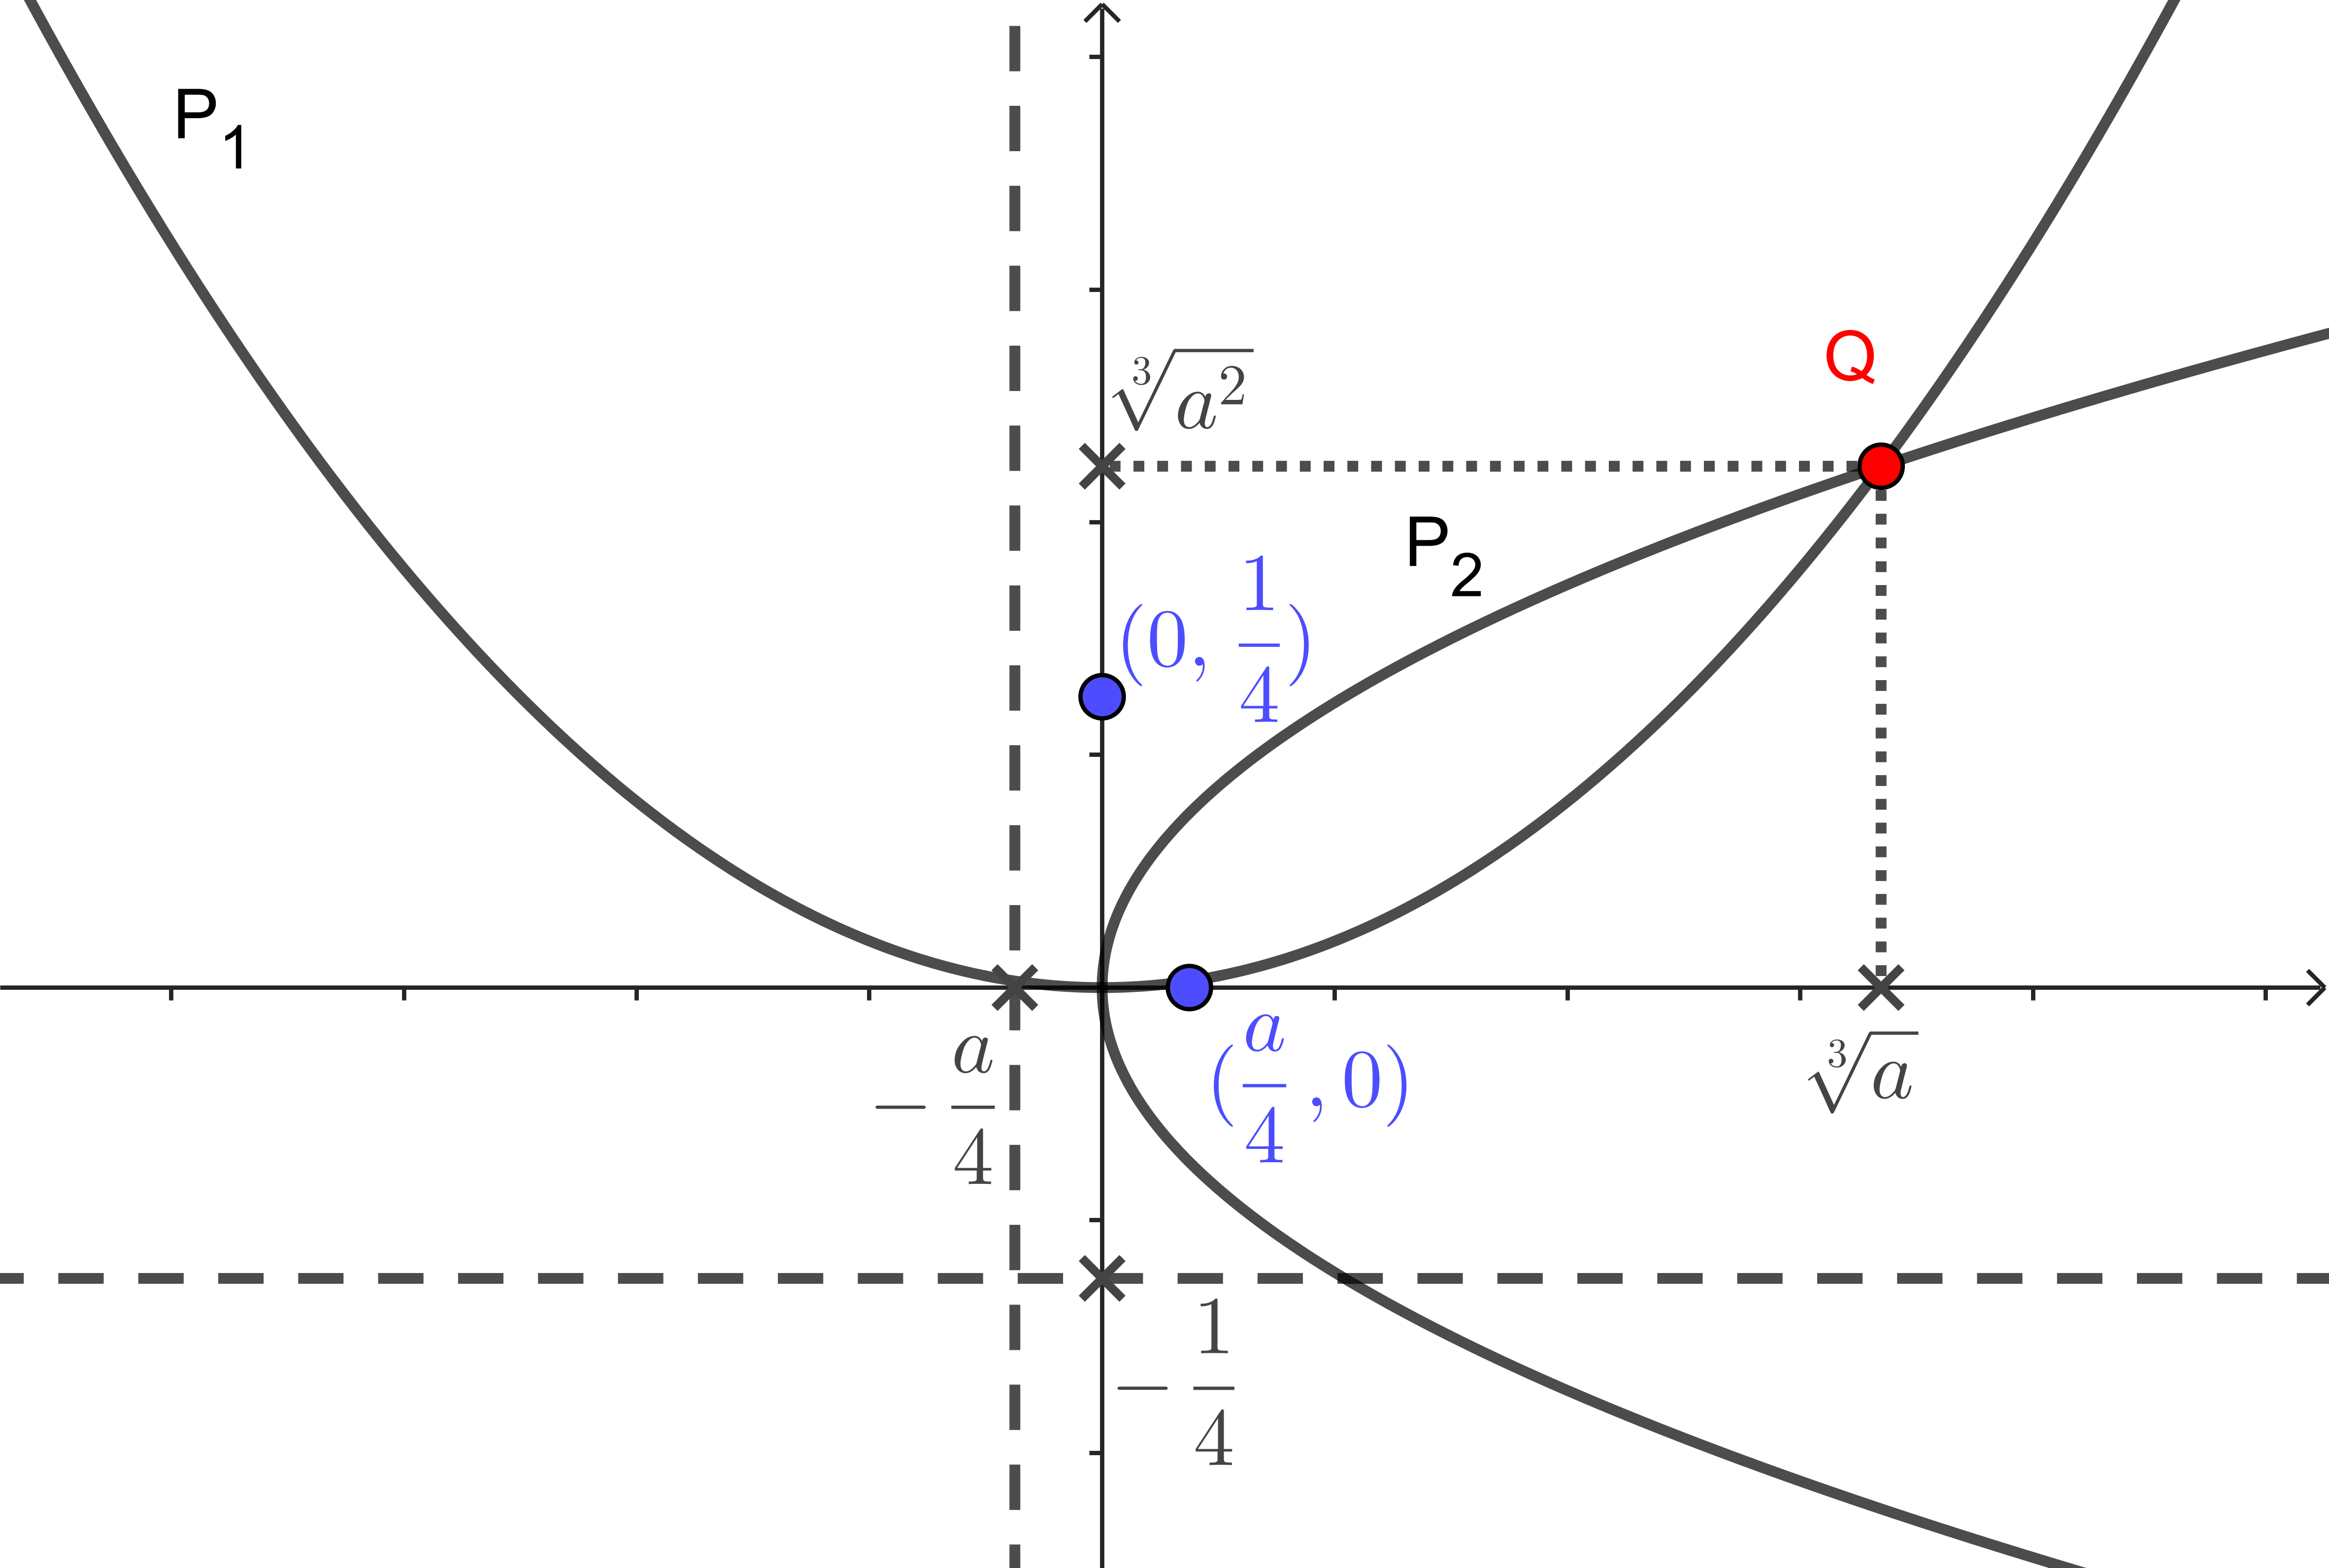
\includegraphics[width=0.7\textwidth]{images/starogr_problemi/cube_parabola.png}
    \caption[Menehmova konstrukcija kubičnega korena]{Menehmova konstrukcija števila $\sqrt[3]{2}$ preko parabol. Vzeto iz~\cite[str.\ 6]{videla1997}.}
    \label{fig:videla}
\end{figure}
Presečišči teh dveh parabol dobimo preko enakosti
$$y = x^2 = y^4/a^2,$$
kar nam da enačbo $y(a^2-y^3) = 0$ z rešitvama $y=0$ in $y = \sqrt[3]{a^2}$. Presečišči sta torej koordinatno izhodišče in točka $Q = (\sqrt[3]{a}, \sqrt[3]{a^2}) $. Njena abscisa je naša rešitev.
\opomba{Čeprav je konstrukcija enostavna in logična, je izvedljiva le v teoriji, saj z roko ne znamo natančno risati parabol.}

\subsubsection*{Martinova konstrukcija}

George E.\ Martin v~\cite[str.\ 156--157]{geometricconstructions} poda preprosto konstrukcijo števila $\sqrt[3]{k}$ za poljubno origami število $k$. Tudi on pri tem uporabi dve paraboli, vendar pri postopku potrebujemo le njuni gorišči in premici vodnici. Ne bomo iskali njunih presečišč, temveč bomo z Belochinim pregibom konstruirali njuno skupno tangento, ki nam bo podala željeni rezultat.

Naj bo $k \in $ poljuben. Vzemimo paraboli z goriščema v točkah $P = (-1, 0)$ in $Q = (0, -k)$ ter premici vodnici $p: x = 1$ in $q: y = k$. Paraboli imata skupno gorišče v koordinatnem izhodišču in sta pravokotni druga na drugo, torej imata eno samo skupno tangento. Prepognimo točko $P$ na premico $p$ in točko $Q$ na premico $q$. Pregib seka $y$-os v točki $R$ (slika~\ref{fig:martin}).
\begin{figure}[h]
    \centering
    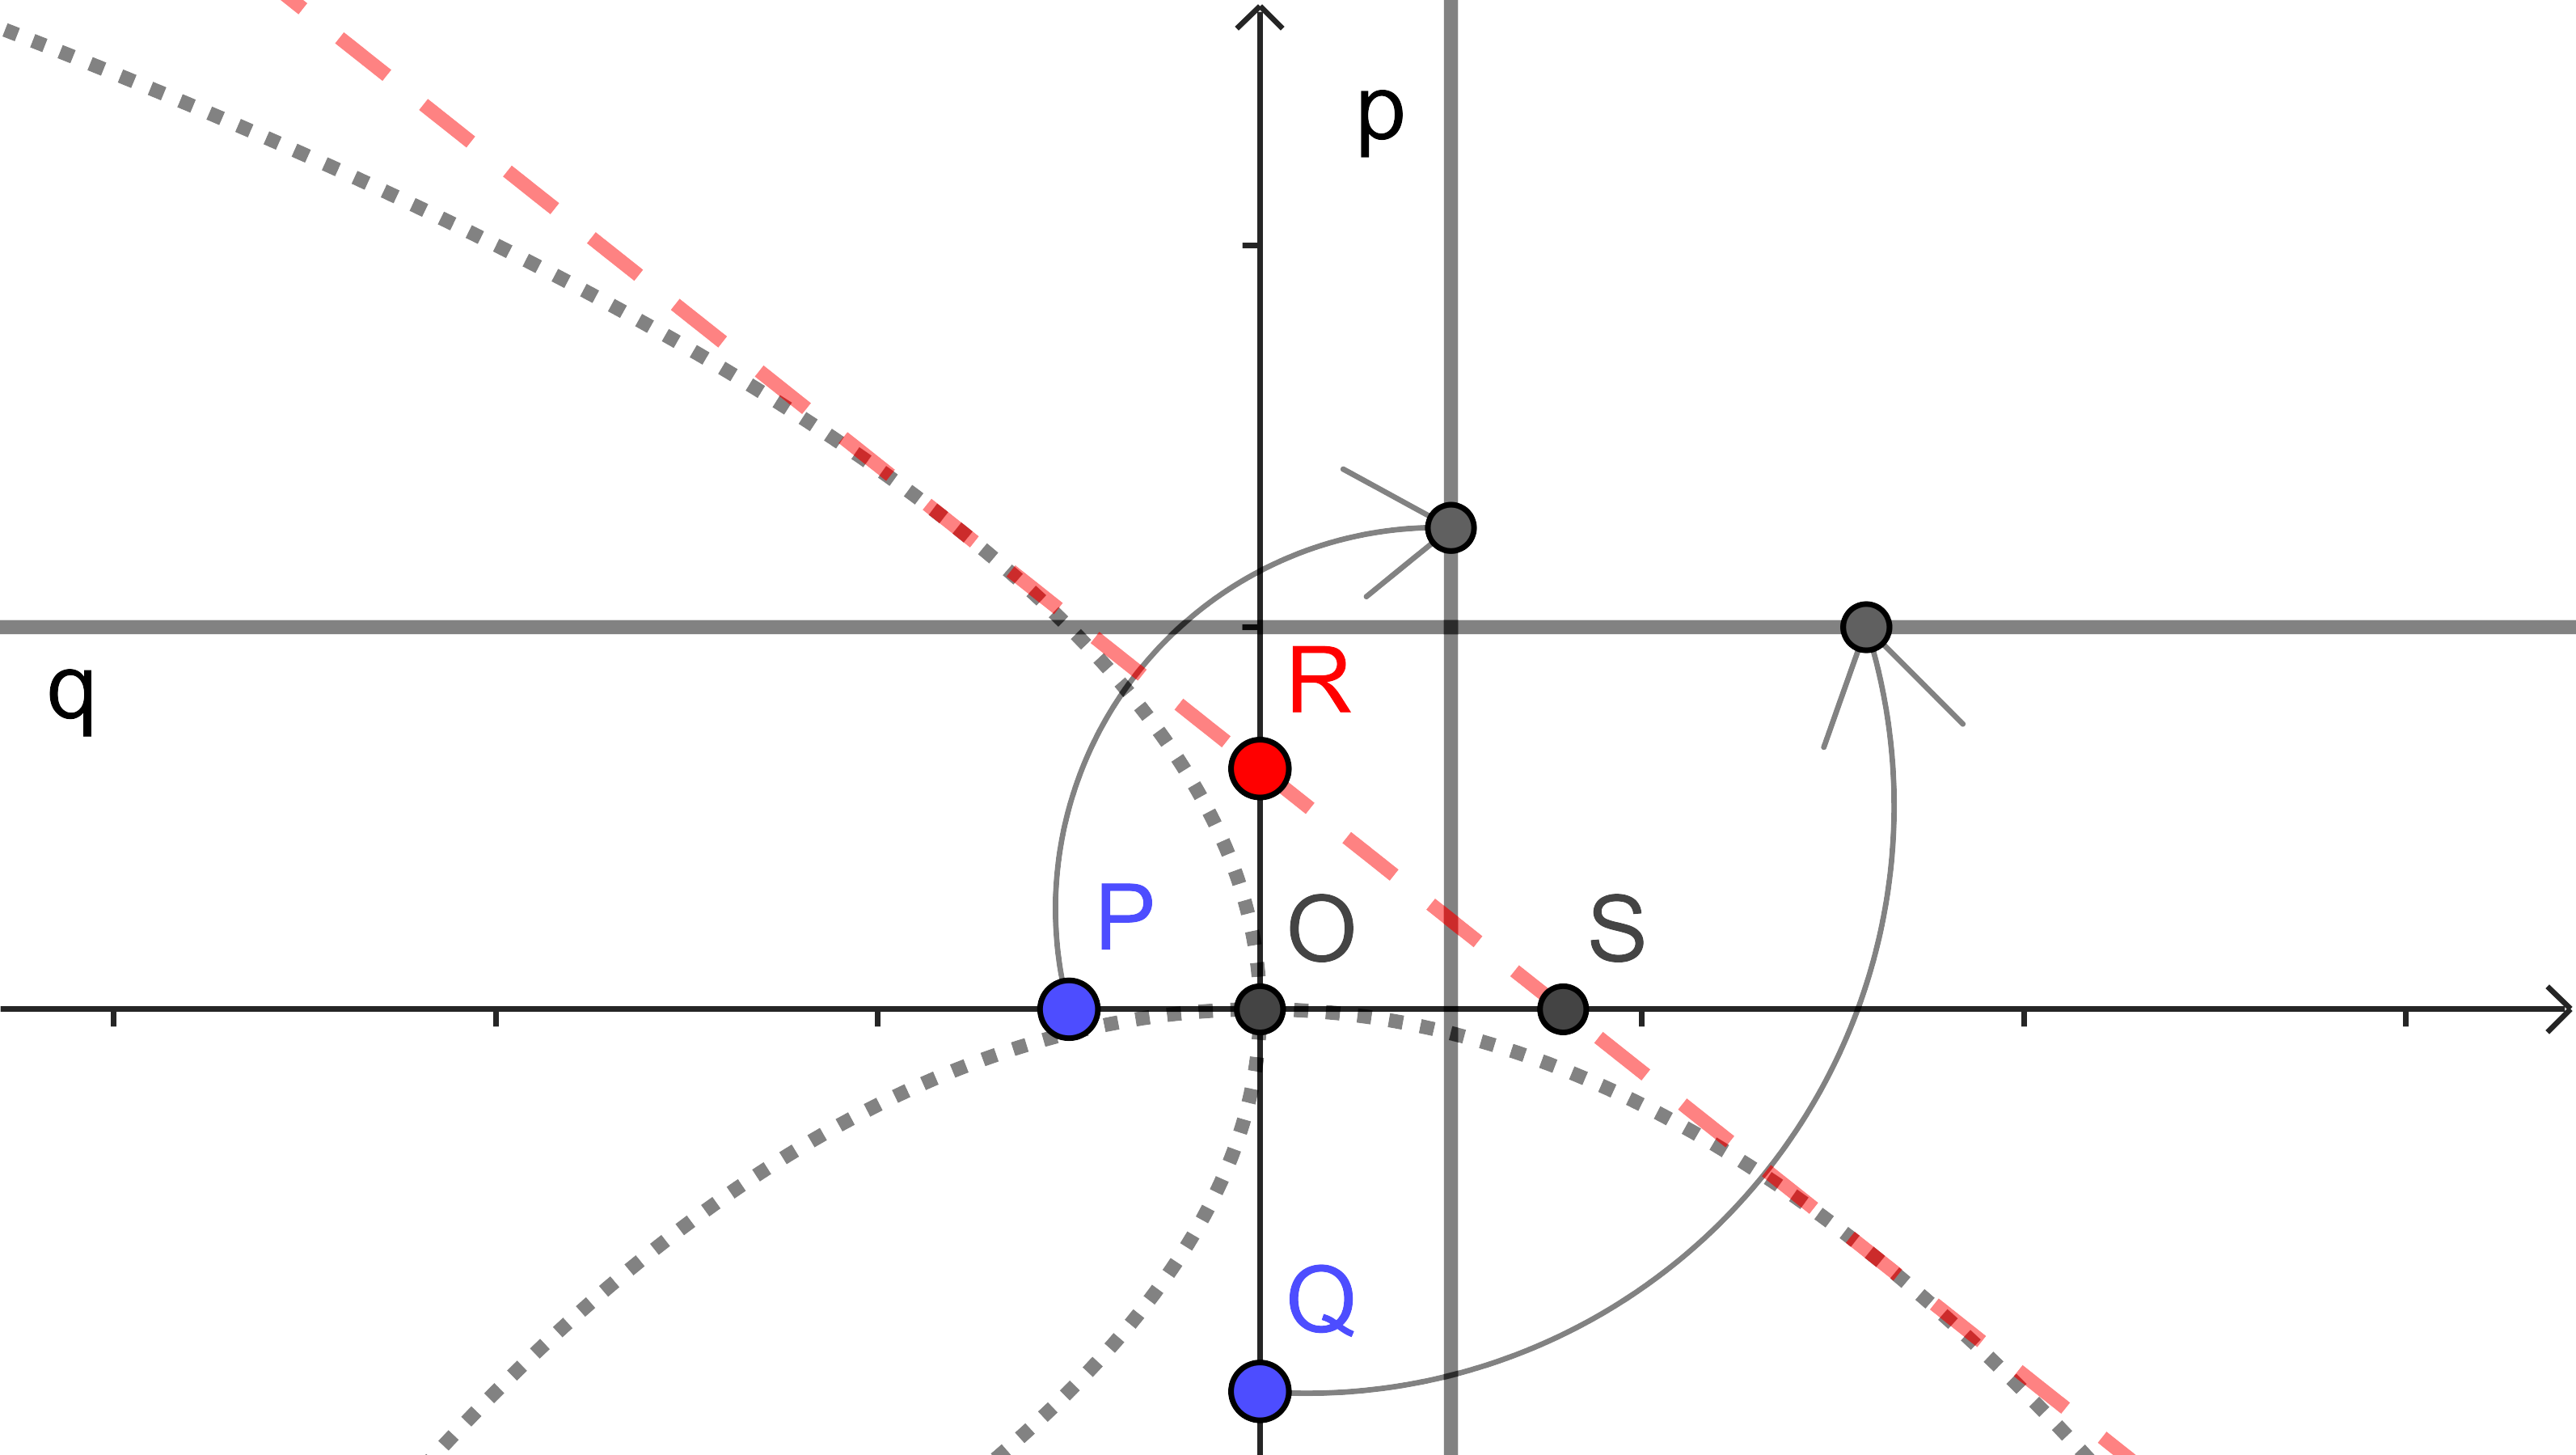
\includegraphics[width=0.6\textwidth]{images/starogr_problemi/cube_martin.png}
    \caption[Martinova konstrukcija kubičnega korena]{Martinova konstrukcija števila $\sqrt[3]{k}$.}
    \label{fig:martin}
\end{figure}
\begin{trditev}
    Točka $R$ iz zgornje konstrukcije ima koordinate $(0, \sqrt[3]{k})$.
\end{trditev}
\begin{dokaz}
    Označimo z $O$ koordinatno izhodišče in s $S$ presečišče pregiba z $x$-osjo. Točki $R$ in $S$ sta zaradi take izbire gorišč in premic vodnic ravno središči daljic z enim krajiščem v točkah $P$ in $Q$ ter drugim krajiščem v njunih slikah. Torej velja $PR \perp RS \perp SQ$. Zato so trikotniki $\triangle POR, \triangle ROS$ in $\triangle SOQ$ podobni. Iz tega ob upoštevanju $|OP| = 1$ in $|OQ| = k$ dobimo razmerje
    $$ \frac{|OR|}{|OP|} = \frac{|OS|}{|OR|} = \frac{|OQ|}{|OS|} \Longrightarrow |OR| = \frac{|OS|}{|OR|} = \frac{k}{|OS|}, $$
    iz česar sledi
    $$ |OR|^3 = |OR| \cdot \frac{|OS|}{|OR|} \cdot \frac{k}{|OS|} = k \Longrightarrow |OR| = \sqrt[3]{k}.$$
\end{dokaz}
\begin{opomba}
    V razdelku~\ref{podpogl:beloch_kvadrat_koren} bomo spoznali konstrukcijo števila $\sqrt[3]{2}$ preko Belochinega kvadrata, ki je v bistvu poseben primer Martinove konstrukcije.
\end{opomba}

\subsubsection*{Messerjeva konstrukcija}

Peter Messer v~\cite{messer1986} navaja avtorski postopek, ki sicer ne konstruira števila $\sqrt[3]{2}$ kot razdaljo, temveč kot razmerje: kvadraten list papirja po horizontali razdelimo na tri dele (to sedaj že znamo storiti) ter točki $p_1$ in $p_2$ s prepogibom položimo na premici $L_1$ in $L_2$, kot kaže slika~\ref{fig:messer} (levo).
\begin{figure}[h]
    \centering
    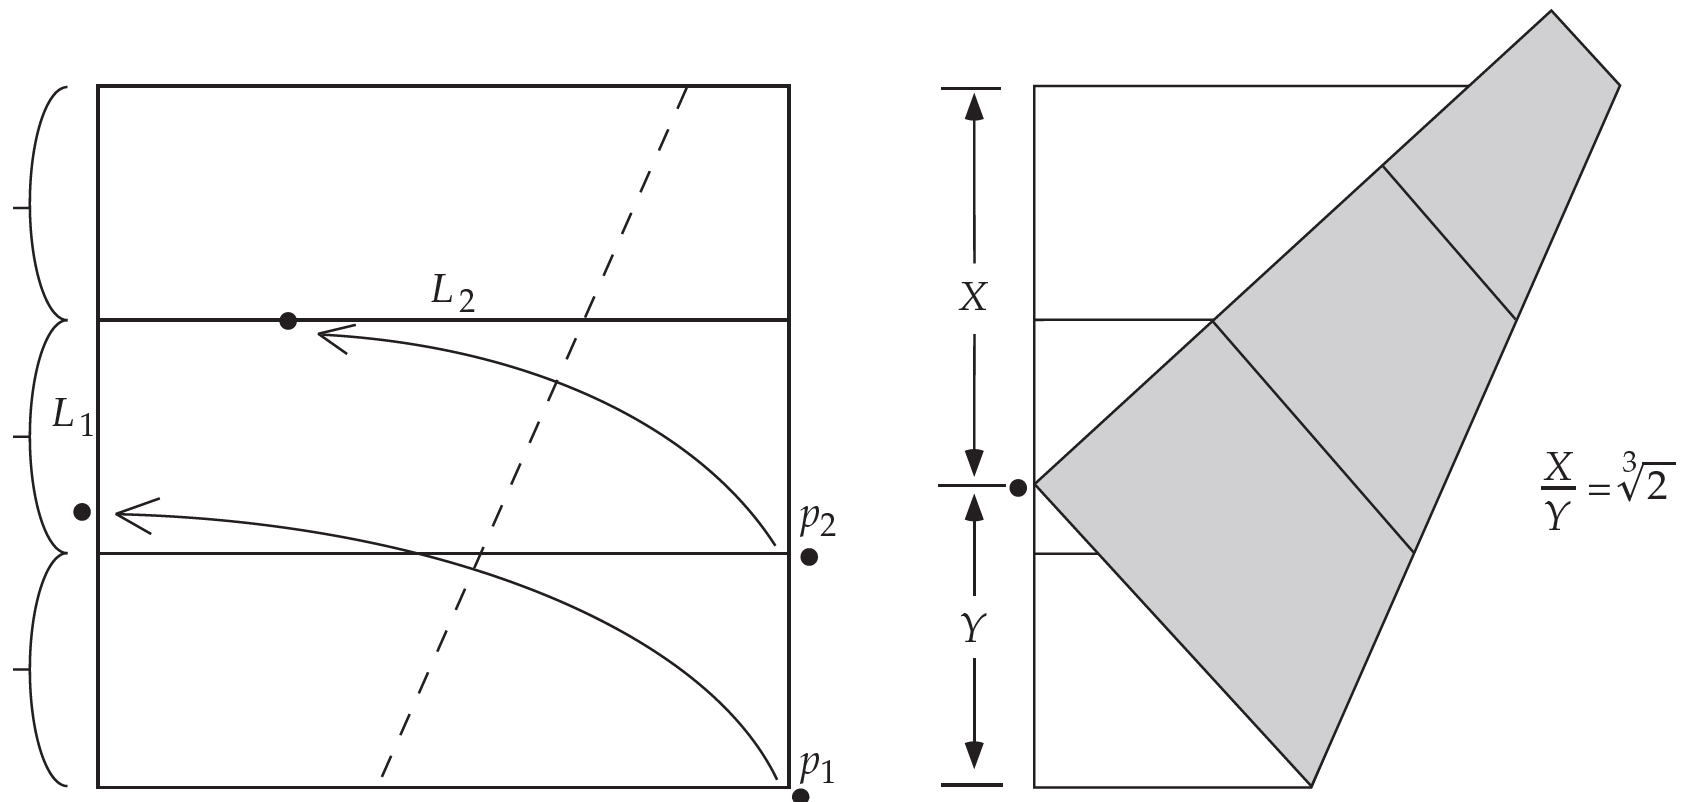
\includegraphics[width=0.68\textwidth]{images/starogr_problemi/messer1.png}
    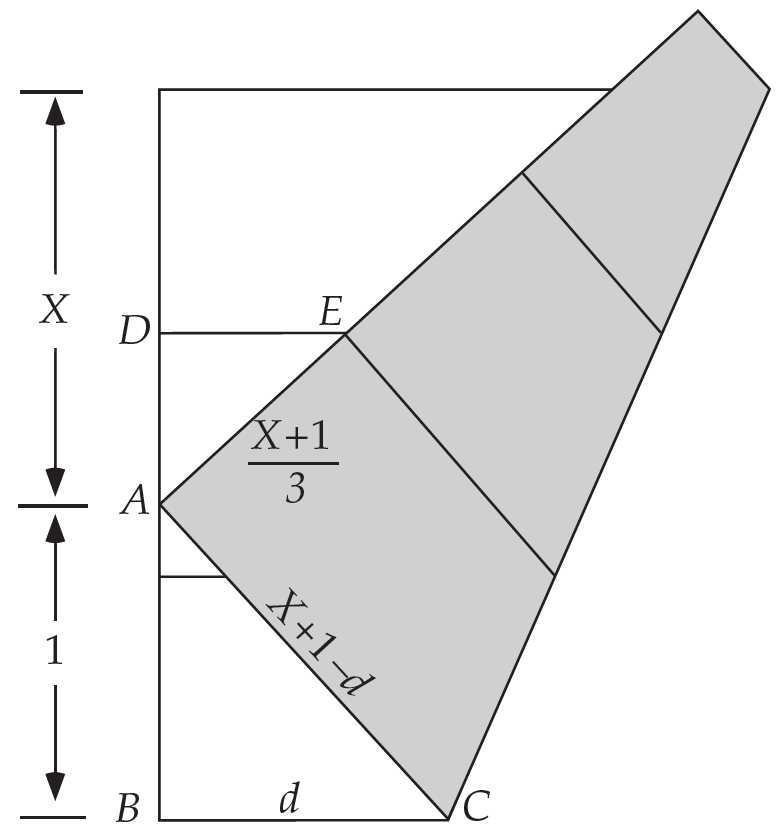
\includegraphics[width=0.3\textwidth]{images/starogr_problemi/messer2.png}
    \caption[Messerjeva konstrukcija]{Messerjeva konstrukcija razmerja $\sqrt[3]{2}$. Vzeto iz~\cite[str.\ 67--68]{hull2013}.}
    \label{fig:messer}
\end{figure}
\begin{trditev}
    Slika točke $p_1$ deli levo stranico kvadrata v razmerju $\sqrt[3]{2}$.
\end{trditev}
\begin{dokaz}
    Vpeljimo oznake $X, Y, A, B, C, D, E$ ter $d = |BC|$, kot kaže slika~\ref{fig:messer}. Dokazati moramo $X/Y = \sqrt[3]{2}$, za lažje računanje pa brez škode privzemimo $Y=1$. Stranica kvadrata je tako dolga $X+1$, zato je $|AC| = X+1-d$ in $|AE| = (X+1)/3$.

    Opazimo podobna pravokotnika $\triangle ABC$ in $\triangle ADE$. Iz trikotnika $\triangle ABC$ s pomočjo Pitagorovega izreka izrazimo $d = (X^2+2X)/(2X+2)$, preko leve stranice pa še $|AD| = X - (X+1)/3 = (2X-1)/3$. Iz podobnosti omenjenih trikotnikov izrazimo razmerje katete in hipotenuze z enačbo $|BC|/|AC| = |AD|/|AE|$. Ko vstavimo noter vse vrednosti, odvisne od $X$, dobimo enačbo
    $$ \frac{X^2 + 2X}{X^2 + 2X + 2} = \frac{2X - 1}{X + 1},$$
    ki se nam poenostavi prav v $X^3 = 2$. Torej je $X = \sqrt[3]{2}$.
\end{dokaz}
\opomba{Lahko bi rekli, da poleg razmerja v primeru $Y=1$ Messer konstruira razdaljo $\sqrt[3]{2}$, vendar je razdalja $Y$ odvisna od stranice kvadrata. V tem primeru bi morali vzeti kvadraten list papira s stranico $1 + \sqrt[3]{2}$, za kar bi pač potrebovali že konstrukcijo kubičnega korena števila $2$. Da bi pri splošnem kvadratnem listu papirja dobili to dolžino, moramo razdalji $X$ in $Y$ z origamijem še deliti, to pa že znamo.}

\subsection{Trisekcija kota}
\label{podpogl:trisekcija}

Kot $90^\circ$ znamo tretjiniti z neoznačenim ravnilom in šestilom, saj znamo konstruirati kot $30^\circ$. Vem pa že, da ne obstaja konstrukcija, s katero na tri skladne kote razdelimo \emph{poljuben} kot -- v razdelku~\ref{podpogl:evkl_konstruktibilnost} smo dokazali neobstoj origami konstrukcije za trisekcijo kota $60^\circ$.

% SPODNJI DOKAZ JE PREPISAN IZ VIRA IN SAMO CITIRAN V prejšnjem odstavku

% Algebraični dokaz, da z evklidskim orodjem ne moremo tretjiniti poljubnega kota -- dokažimo za kot $60°$. (iz~\cite[str.\ 77--78]{jerman1998})

% Kot $60°$ znamo narisati. Če bi ga znali razdeliti na tri enake dele, bi potemtake znali narisati tudi kot $20°$, s tem pa (ker znamo risati pravokotnice) tudi $\cos 20°$ \textcolor{red}{slika z enotsko krožnico}. Pokažimo, da to ne gre.

% Izračunajmo minimalni polinom števila $\cos 20°$. Ker je
% $$ \frac{1}{2} = \cos 60° = \cos(3 \cdot 20°) = 4 \cos^3 20° - 3 \cos 20°, $$
% ima polinom $ p(x) = 8 x^3 - 6x - 1 $ ničlo $ \cos 20°$. Minimalni polinom števila $ \cos 20°$ deli polinom $p$. Če polinom $p$ razpade na produkt dveh polinomov s koeficienti v $\Q$, je eden od polinomov zagotovo linearen. To pa bi pomenilo, da ima polinom $p$ vsaj eno racionalno ničlo. Edini kandidatki za racionalne ničle polinoma $p$ so števila iz množice
% $$ \{\pm 1, \pm \frac{1}{2}, \pm \frac{1}{4}, \pm \frac{1}{8} \}. $$ Nobeno od teh števil ni ničla polinoma $p$, zato se $p$ ne da razcepiti na produkt dveh polinomov z racionalnimi koeficienti. Minimalni polinom števila $ \cos 20°$ je torej enaka
% $$ m(x) = \frac{1}{8} p(x) = x^3 - \frac{3}{4} x - \frac{1}{8}. $$
% Tako je razsežnost prostora $\Q(\cos 20°)$  nad obsegom $\Q$ enaka $3$ in števila $ \cos 20° $ se ne da narisati le z ravnilom in šestilom.

% Zato trisekcija kota v splošnem ni mogoča.

\subsubsection*{Starogrška rešitev preko presečišča krožnice in hiperbole}

Grki so tudi ta problem uspeli rešiti s stožnicami. Videla v~\cite[str.\ 6--7]{videla1997} opisuje Pappusovo konstrukcijo iz $3$.\ stoletja po Kr., ki je tu ne bomo dokazali. Gre za sledeč postopek: Na kraku $BA$ poljubnega kota $\angle ABC$ izberemo poljubno točko $F$ in zarišemo krožnico s središčem v točki $B$ in polmerom $BF$. Naj bo $BD$ simetrala kota $\angle ABC$. Naj bo točka $E$ presečišče krožnice in hiperbole z ekscentičnostjo $2$, ki ima gorišče v točki $F$ in premico vodnico $BD$ (slika~\ref{fig:trisection_gr}). Potem poltrak $BE$ tretjini kot $\angle ABC$.

\begin{figure}[h]
    \centering
    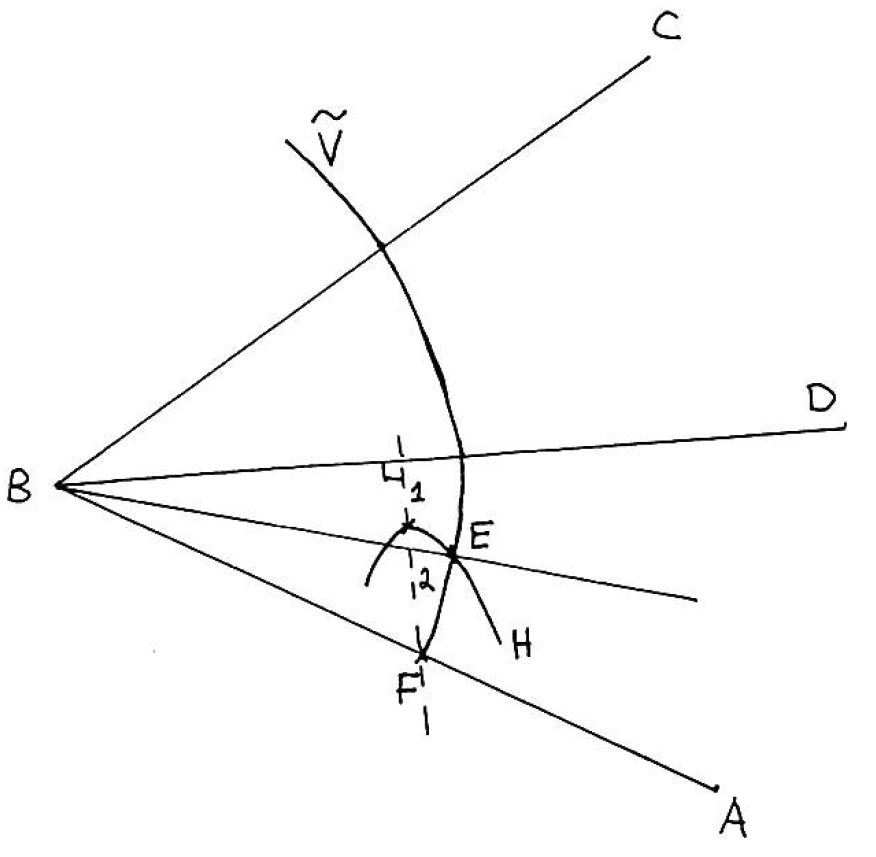
\includegraphics[width=0.5\textwidth]{images/starogr_problemi/trisection_grska.png}
    \caption[Pappusova trisekcija kota]{Pappusova trisekcija kota preko stožnic. Vzeto iz~\cite[str.\ 7]{videla1997}.}
    \label{fig:trisection_gr}
\end{figure}

\subsubsection*{Abejeva metoda}

Sledeča metoda ima ime po japonskemu matematiku Hisashiju Abeju, ki jo je odkril v $80$-ih letih prejšnjega stoletja. Postopek vključuje Belochin pregib, torej se ga ne da izvesti z evklidskim orodjem, edina pomankljivost metode pa je, da deluje le za ostre kote. Postopek je sledeč:

\begin{enumerate}
    \item Na kvadratnem listu papirja konstruiramo poljuben kot $\theta$, ki ima vrh v spodnjem desnem vogalu in en krak na spodnji stranici. Nato konstruiramo še dva horizontalna in ekvidistančna pregiba na dnu papirja (slika~\ref{fig:abe_1} levo).
    \item Točko $p_1$ prepognemo na spodnji horizontalen pregib, označen $L_1$, točko $p_2$ pa na poševen krak kota, označen z $L_2$ (slika~\ref{fig:abe_1} na sredi).
    \item Preden pregib razgrnemo, podaljšamo pregib $L_1$ do konca in nov pregib označimo z $L_3$ (slika~\ref{fig:abe_1} desno).
    \item Papir razgrnemo in tokrat v spodnji levi kot podaljšamo pregib $L_3$.
\end{enumerate}
\begin{figure}[h]
    \centering
    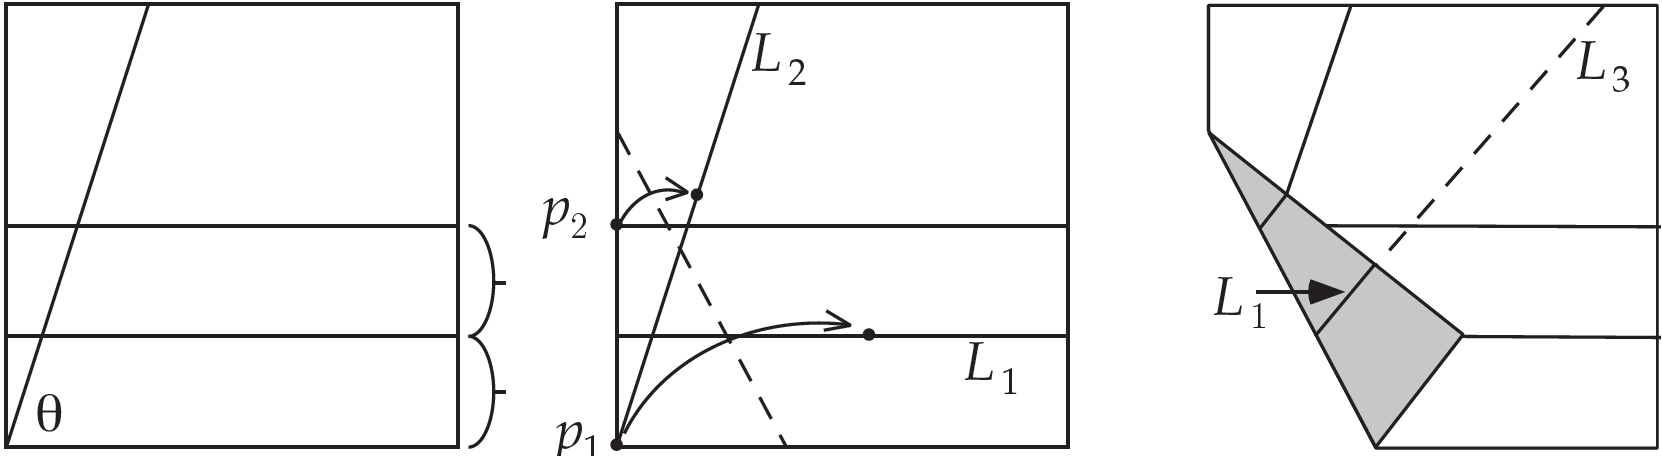
\includegraphics[width=0.95\textwidth]{images/starogr_problemi/abe_nastavek1.png}
    \caption[Abejeva metoda ($1$.\ del)]{Trisekcija kota po Abejevi metodi. Vzeto iz~\cite[str.\ 64]{hull2013}.}
    \label{fig:abe_1}
\end{figure}

\opomba{V $3$.\ koraku opravimo pregib še preden smo razgrnili prvega. To je za nas načeloma prepovedana poteza, vendar bi se dalo $L_3$ konstruirati tudi po klasični poti z enkratnimi prepogibi -- označili bi sliko točke, ki leži hkrati na $L_1$ in levi stranici kvadrata, ter točko v pregibu iz $2$.\ koraka, ki leži na $L_1$ in skozinju naredili pregib $L_3$ -- zato zaradi lažje izvedbe brez škode dopustimo tak postopek.}

\begin{trditev}
    Pregib $L_3$ poteka skozi točko $p_1$. Kot s krakoma $L_2$ in $L_3$ ter vrhom v točki $p_1$ je velik $\theta/3$.
\end{trditev}
\begin{posledica}
    Ko spodnji rob kvadrata prepognemo na pregib $L_3$, razdelimo kot $\theta$ na tri skladne kote.
\end{posledica}

\begin{dokaz}
    Posledica logično sledi, zato dokazujemo le trditev. Označimo z $x$ točko, ki leži na presečišču pregiba $L_1$ in pregiba iz $2$.\ koraka Abejeve metode. Z $A, B$, in $C$ označimo še slike točk z leve stranice kvadrata, kot kaže slika~\ref{fig:abe_2}.
    \begin{figure}[h]
        \centering
        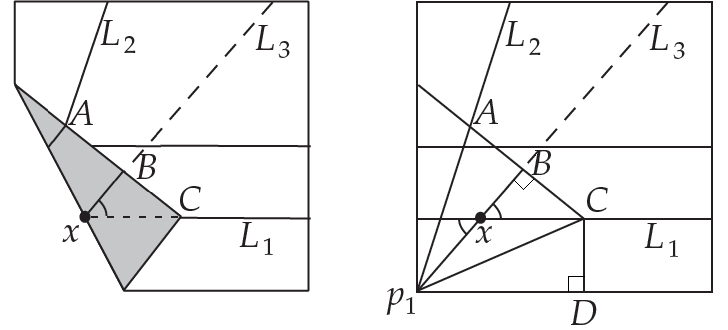
\includegraphics[width=0.7\textwidth]{images/starogr_problemi/abe_trisekcija.png}
        \caption[Abejeva metoda ($2$.\ del)]{Dokazovanje Abejeve metode. Vzeto in predelano iz~\cite[str.\ 65]{hull2013}.}
        \label{fig:abe_2}
    \end{figure}
    Ker je točka $C$ slika točke $p_1$ in $x$ leži na $L_1$, daljica $xC$ leži na $L_1$. Po konstrukciji daljica $xB$ leži na $L_3$, zato sta kota ob $x$, ko papir razgrnemo, skladna. Zaradi sovršnosti kotov daljica $p_1x$ leži na $L_3$, s čimer je prvi del trditve dokazan.
    
    Na razgrnjenem papirju zarišemo (ali prepognemo) še nekaj daljic (slika~\ref{fig:abe_2} desno). Ker velja $|AB| = |BC| = |CD|$ in imata pravokotna trikotnika $\triangle p_1AB$ in $\triangle p_1BC$ skupno še drugo kateto, trikotnika $\triangle p_1BC$ in $\triangle p_1CD$ pa skupno hipotenuzo, so vsi trije trikotniki skladni z enakim kotom v točki $p_1$, torej nam pregiba skozi daljici $p_1B$ (kar je ravno $L_3$) in $p_1C$ kot $\theta$ razdelijo na tri skladne kote.
\end{dokaz}

Ker ta postopek deluje le za ostre kote, si poglejmo naslednjo metodo, ki jo lahko uporabljamo tako za ostre kot tudi tope kote.

\subsubsection*{Justinova metoda}

Francoski matematik Jacques Justin za svojo metodo trisekcije ne zahteva kvadratnega lista papirja, ampak je dovolj kakršenkoli list. Lang v~\cite[str.\ 34]{lang2013} takole navaja njegovo kosntrukcijo:

Na sredo narišemo poljuben kot $\angle ABC$ (oster ali top) in njuna kraka podaljšamo skozi vrh $B$. Skozi vrh konstruiramo poltrak, pravokoten na krat $BA$. Točko $C$ prezrcalimo čez vrh v točko $D$ ter nato obe točki prepognemo na nosilko kraka $BA$ in ravno konstruirano pravokotnico, kot kaže slika~\ref{fig:justin} (levo). Nazadnje na Belochin pregib konstruiramo še pravokotnico skozi točko $B$.
\begin{figure}[h]
    \centering
    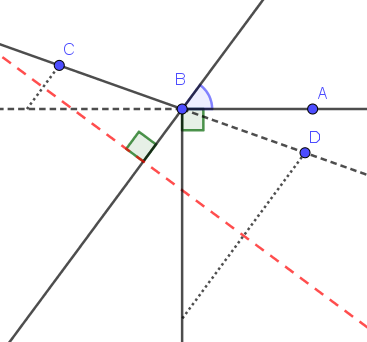
\includegraphics[width=0.45\textwidth]{images/starogr_problemi/justin_trisection.png}
    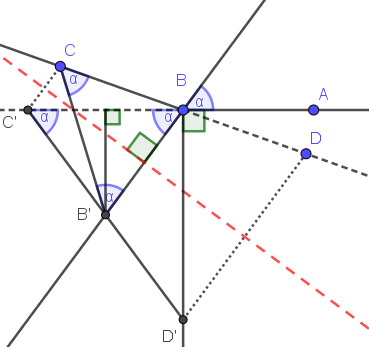
\includegraphics[width=0.45\textwidth]{images/starogr_problemi/justin_trisection_dokaz.png}
    \caption[Justinova trisekcija kota]{Justinova trisekcija kota (levo) in njen geometrijski dokaz (desno).}
    \label{fig:justin}
\end{figure}

\begin{trditev}
    Kot, ki v točki $B$ oklepata zadnja pravokotnica iz zgornje konstrukcije in krak $BA$, je tretjina kota $\angle ABC$.
\end{trditev}
\begin{dokaz}
    Označimo z $\alpha$ kot iz trditve. Naj bosta točki $C'$ in $D'$ sliki točk $C$ in $D$, točka $B'$ pa presečišče daljice $C'D'$ s pravokotnico iz trditve. Po konstrukciji Belochinega pregiba je daljica $C'D'$ slika daljice $CD$, torej je točka $B'$ slika točke $B$. Točka $B'$ je tako središče daljice $C'D'$ in zato je vzporednica k poltraku $BD'$ skozi točko $B'$ simetrala daljice $C'B$. Trikotnik $\triangle C'B'B$ je tako enakokrak in velja $\angle C'BB' = \angle B'C'B = \alpha$.
    
    Ker sta trikotnika $\triangle C'B'B$ in $\triangle CBB'$ zaradi simetričnosti glede Belochin pregib skladna, velja tudi $\angle B'CB = \angle CB'B = \alpha$. Iz vsote notranjih kotov trikotnike $\triangle CB'B$ sledi $\angle C'BC = 180^\circ - 3\alpha$, torej je $\angle ABC = 180^\circ - \angle C'BC = 3\alpha$. 
\end{dokaz}

\subsubsection*{Martinovi konstrukciji za trisekcijo ostrega kota}

George E.\ Martin v~\cite[poglavje 10]{geometricconstructions} navaja še dve metodi za trisekcijo ostrega kota.

Pri prvi vzamemo oster kot $\angle PQR$ in s točko $M$ označimo središče daljice $PQ$. Skozi $M$ konstruiramo pravokotnico $p$ na $QR$, nato pa še pravokotnico na $p$. Opravimo tisti Belochin pregib (od treh možnih), ki seka daljico $PM$ in točko $Q$ položi na premico $q$ (v točko $Q'$), točko $P$ pa na premico $p$ (v točko $P'$). S $T$ označimo presečišče daljice $QQ'$ s premico $p$ in s $S$ presečišče pregiba s premico $q$ (slika~\ref{fig:trisection_10.4}).

\begin{figure}[h]
    \centering
    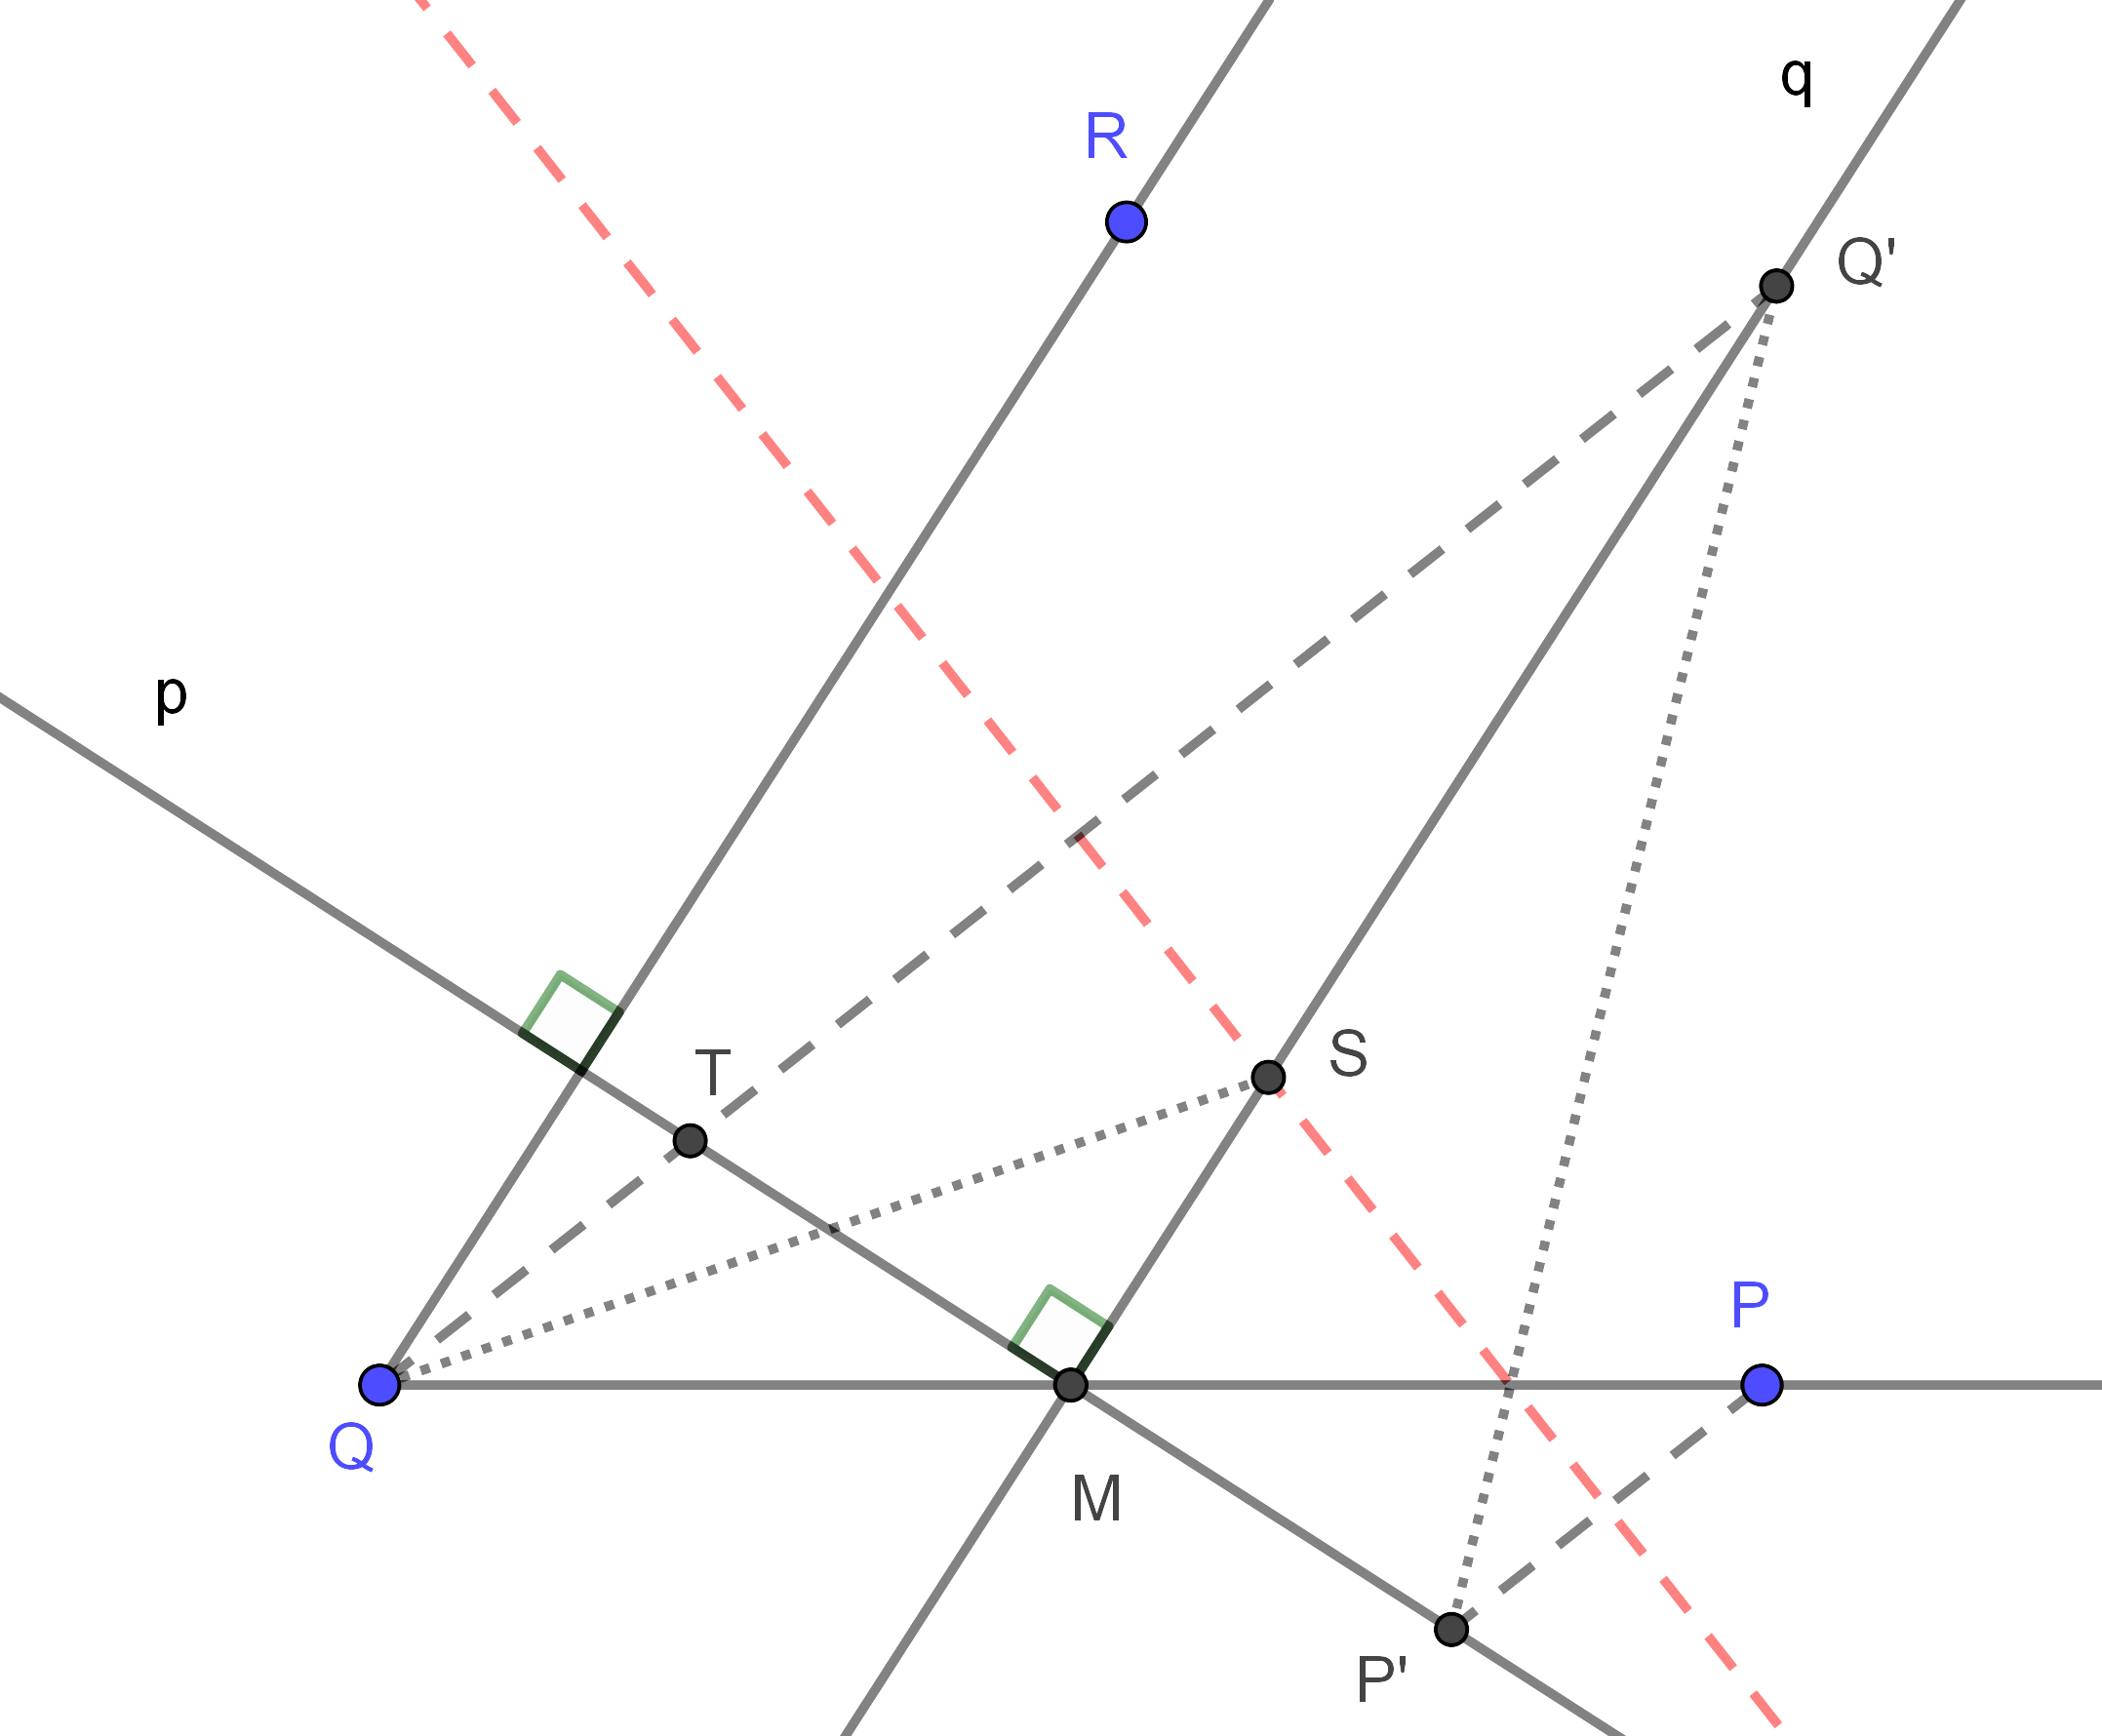
\includegraphics[width=0.5\textwidth]{images/starogr_problemi/trisection_10.4.png}
    \caption[Martinova trisekcija ostrega kota (metoda $1$)]{Martinov postopek za trisekcijo kota iz~\cite[str.\ 154]{geometricconstructions}.}
    \label{fig:trisection_10.4}
\end{figure}

\begin{trditev}
    Daljici $QT$ in $QS$ tretjinita kot $\angle PQR$.
\end{trditev}
\begin{dokaz}
    Ker velja $|QM| = |MP|$, $\angle PMP' = \angle TMQ$ in $QT \parallel PP'$, sta trikotnika $\triangle QMT$ in $\triangle PMP'$ skladna in je $|TM| = |MP'|$. Potem sta skladna tudi pravokotna trikotnika $\triangle TMQ'$ in $\triangle P'MQ'$, zato je $\angle MQ'P' = \angle TQ'M = \angle RQQ'$ (zaradi izmeničnih kotov ob vzporednicah $QR$ in $q$) $= \angle Q'QS$ (ker je trikotnik $\triangle QSQ'$ enakokrak).
    
    Bralec se lahko hitro prepriča, da daljica $Q'P'$ seka pregib ravno v njegovem presečišču z daljico $MP$ (vsi koti ob tem presečišču so zaradi konstrukcija pregiba in sovršnosti skladni). Zato velja še $\angle PQQ' = \angle P'Q'Q$, iz česar sledi
    $$ \angle MQS = \angle SQT = \angle TQR.$$
\end{dokaz}

Druga metoda je prvi zelo podobna. Zopet vzamemo oster kot $\angle PQR$ in s točko $M$ označimo središče daljice $PQ$. Naj bo $l$ pravokotnica na $QR$ skozi točko $Q$, točka $N$ nožišče pravokotnice na premico $l$ skozi točko $P$, s $q$ označimo pa še pravokotnico na premico $l$ skozi točko $M$. Opravimo tisti Belochin pregib, ki točko $Q$ položi na premico $q$ (v točko $Q'$) in točko $N$ na poltrak $QR$. Naj bo točka $S$ presečišče pregiba s premico $q$ (slika~\ref{fig:trisection_10.14}).

\begin{figure}[h]
    \centering
    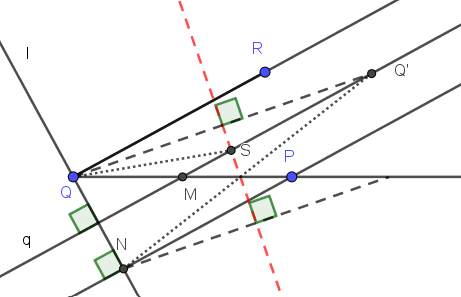
\includegraphics[width=0.6\textwidth]{images/starogr_problemi/trisection_10.14.png}
    \caption[Martinova trisekcija ostrega kota (metoda $2$)]{Martinov postopek za trisekcijo kota iz~\cite[str.\ 158--159]{geometricconstructions}.}
    \label{fig:trisection_10.14}
\end{figure}

\begin{trditev}
    Daljici $QQ'$ in $QS$ tretjinita kot $\angle PQR$.
\end{trditev}
\begin{dokaz}
    Zopet premislimo, da se pregib, poltrak $QP$ in daljica $NQ'$ sekajo v isti točki. Zato je $\angle QQ'N = \angle PQQ'$. Zaradi vzporednosti kraka $QR$ in premice $q$ sta skladna tudi izmenična kota $\angle RQQ'$ in $\angle QQ'S$, z njima pa je zaradi enakokrakosti trikotnika $\triangle QSQ'$ skladen tudi kot $\angle SQQ'$.

    Ker velja $|QM| = |MP|$ in $q \parallel NP$, je premica $q$ simetrala daljice $QN$, torej tudi simetrala kota $\angle QQ'N$. Iz tega sledi
    $$ \angle MQS = \angle SQQ' = \angle Q'QR.$$
\end{dokaz}
\newpage
\section{Pregibanje tangent na stožnice}
\label{pogl:stoznice}

\textcolor{red}{A čmo premaknit to poglavje tik pred enačbe?}

Iz didaktičnega vidika zelo zanimivo poglavje nam predstavlja konstrukcije tangent na stožnice s prepogibanjem papirja. Vsebina je tu predstavljena tako, da je bralec najprej povabljen, da vzame list papirja in ga prepogiba po navedenih korakih. Po opažanju, kaj se na papirju pri tem prikaže, preidemo na matematični del, kjer dokažemo, da so prepogibi res tangente na določeno stožnico.

Učitelji matematike so povabljeni, da si pri obravnavi stožnic vzamejo čas in izvedejo spodnje aktivnosti. Dijaki bodo z veliko verjetnostjo presenečeni nad rezultati zgibanja, kar jih lahko bolj motivira za obravnavo geometričnih lastnosti stožnic. Priporočljiva je tudi izvedba ure v računalniški učilnici, kjer lahko vsak dijak z ustreznim programskim orodjem (npr.\ Geogebra) sam poskusi zgraditi opisano konstrukcijo. S tem lahko znanje o stožnicah le še bolj utrdi.

Z origamijem ne moremo konstruirati gladkih krožnih lokov. Kljub temu pa lahko z upoštevanjem določenih korakov konstruiramo premice, ki so tangentne na neko krivuljo. Več takih tangent nam poda nekakšno lomljenko, če pa bi konstrukcije pregibov ponavljali v nedogled, bi v limiti res dobili gladko krivuljo. Pa si poglejmo, kako s prepogibi dobimo obliko stožnic. \textcolor{red}{envelope oz.\ ovojnica:} \url{https://en.wikipedia.org/wiki/Envelope_%28mathematics%29}

\subsection{Krožnica}

% Tega nikjer v literaturi ni in sem sama dodala. Malo preveč osnovno, ma če se obravnava tiste tri stožnice, pa se lahko kar vse, ane.

\textit{\textbf{Aktivnost:} Vzemi list papirja in svinčnik ter na sredi označi točko $S$. Nato drugje označi še točko $A$. Skozi točko $S$ prepogni poljubno premico in na njej označi točko $A'$, da velja $|SA| = |SA'|$. Nato skozi točko $A'$ prepogni pravokotnico na premico $SA'$. To je iskan pregib. To ponovi čimvečkrat za različno izbiro premice skozi točko $S$ (gl.\ sliko~\ref{fig:koraki_kroznica}). Kaj opaziš?}

\begin{figure}[h]
    \centering
    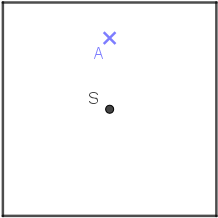
\includegraphics[width=0.3\textwidth]{images/stožnice/folding_kroznica_1.png}
    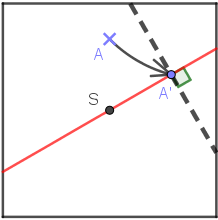
\includegraphics[width=0.3\textwidth]{images/stožnice/folding_kroznica_2.png}
    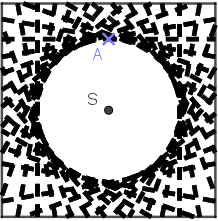
\includegraphics[width=0.3\textwidth]{images/stožnice/folding_kroznica_3.png}
    \caption[Prepogibanje krožnice]{Sukanje izbrane točke okoli središča.}
    \label{fig:koraki_kroznica}
\end{figure}

\opomba{V podpoglavju~\ref{zrcaljenje_origami} smo se naučili prenašati razdalje, zato je zgornja konstrukcija mogoča, zahteva pa še nekaj dodatnih vmesnih pregibov (gl.\ dokaz trditve~\ref{trd:prenasanje_razdalj}).}

Iz konstrukcije pregiba kot pravokotnice na premico $SA'$ skozi točko $A'$ je naslednja trditev očitna in ne potrebuje zapisanega dokaza.

\begin{trditev}
    Konstrukcija iz zgornje aktivnosti nam poda pregib, ki je tangenten na krožnico s središčem v točki $S$ in polmerom $SA$.
\end{trditev}

Za različno izbiro premic skozi točko $S$ dobimo različne tangente in s tem lomljeno krivuljo. S ponavljanjem konstrukcije tangente v neskončnost je krivulja vedno bolj gladka in podobna krožnici.

\subsection{Parabola}

\textit{\textbf{Aktivnost:} Vzemi pravokoten list papirja in svinčnik ter nekje sredi spodnje polovice lista s pisalom označi točko. Nato si izberi točko še na spodnji stranici lista in ga prepogni tako, da se obe izbrani točki prekrijeta. To ponovi čimvečkrat za različno izbiro točke na spodnji stranici papirja (gl.\ sliko~\ref{fig:koraki_parabola}). Kaj opaziš?}

\begin{figure}[h]
    \centering
    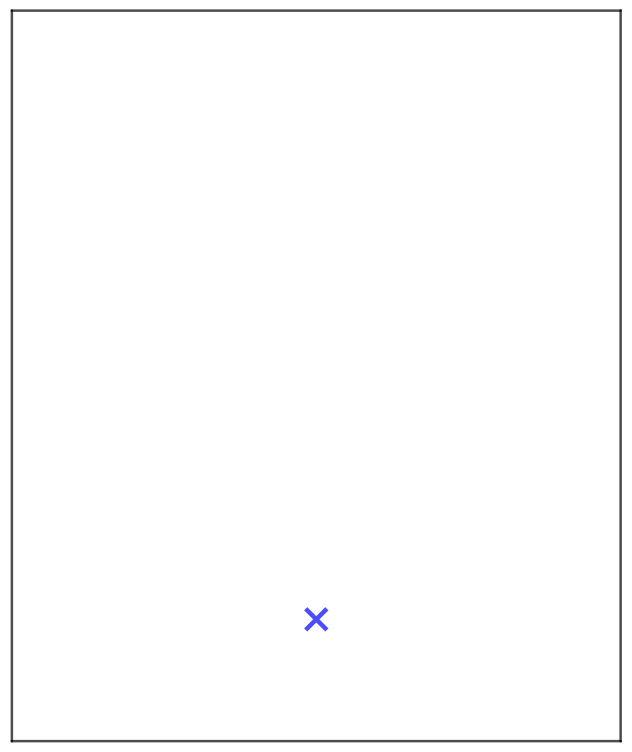
\includegraphics[width=0.3\textwidth]{images/stožnice/folding_parabola_1.png}
    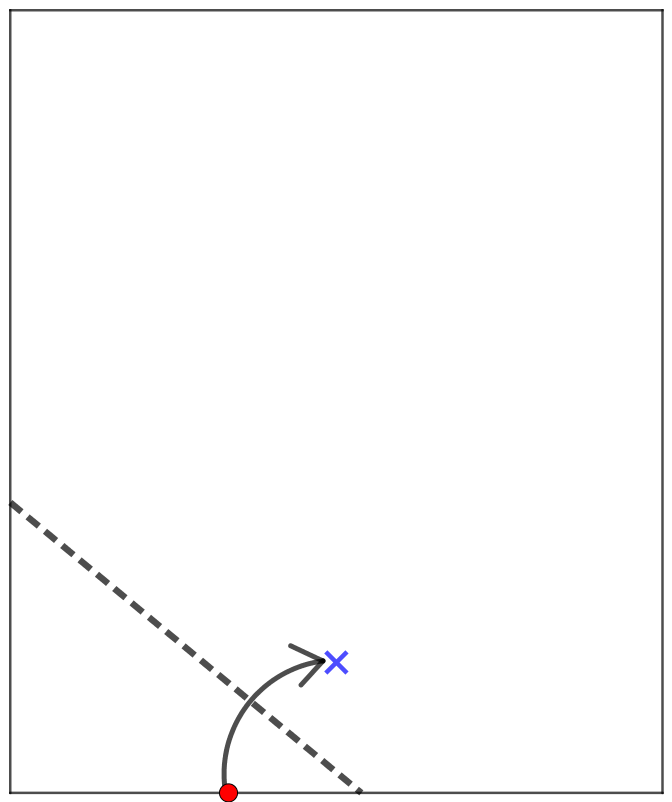
\includegraphics[width=0.3\textwidth]{images/stožnice/folding_parabola_2.png}
    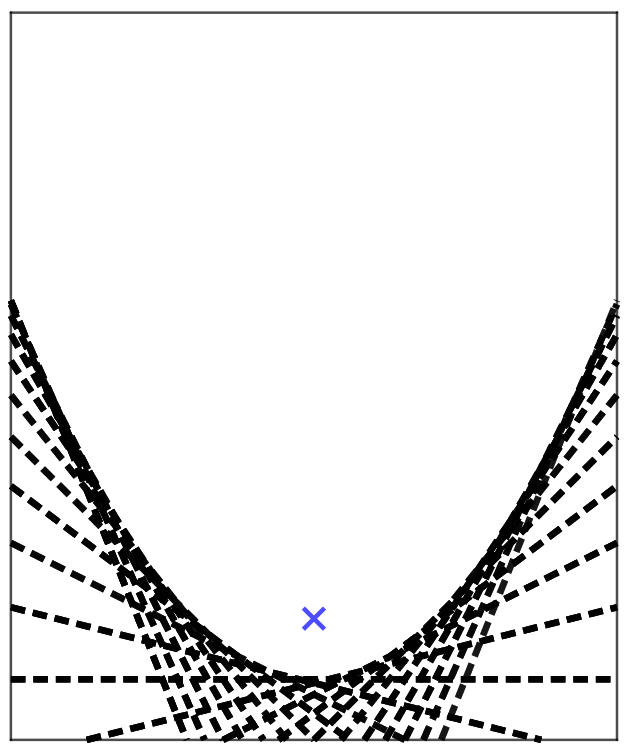
\includegraphics[width=0.3\textwidth]{images/stožnice/folding_parabola_3.png}
    \caption[Prepogibanje parabole]{Prepogibanje spodnje stranice papirja na izbrano točko.}
    \label{fig:koraki_parabola}
\end{figure}

% Najstareši opis zgornje konstrukcije, ker sem jih našla, je v svojo knjigo \emph{Geometric Exercises in Paper Folding} vključil indijski matematik T.\ Sundara Row~\cite{row1917}.
% Hull je našel Row-a (prvič izdana 1893) kot najstarejši zapis te konstrukcije

Omenjen pregib je origami operacija~\ref{op:O3}, lahko pa nanjo gledamo tudi kot na operacijo~\ref{op:O6}. Za le-to smo v poglavju~\ref{pogl:aksiomi} že premislili, da nam pregib, ki poteka skozi dano točko $B$ in točko $A$ položi na premica $a$, poda tangento na parabolo z goriščem $A$ in premico vodnico $a$ (gl.\ sliko~\ref{fig:O6_parabola} in premislek nad njo). Tukaj pa take točke $B$ ni, kar pomeni le to, da smo s pregibom konstruirali neko tangento -- pregib je namreč simetrala daljice, ki ima za krajišči obe izbrani točki iz navodila aktivnosti, torej obstaja točka (točka $P$ na sliki~\ref{fig:O6_parabola}), ki je enako oddaljena od spodnje stranice lista in prve izbrane točke. Nadaljni premislek, da je to edino presečišče pregiba in parabole, je enak kot prej. Spodnja trditev je tako že dokazana.

\begin{trditev}
    Konstrukcija iz zgornje aktivnosti nam poda pregib, ki je tangenten na parabolo z goriščem v izbrani točk in premico vodnico, ki jo predstavlja spodnja stranica lista.
\end{trditev}

Kaj se po večkrat izvedenih pregibih spodnje stranice lista na začetno izbrano točko na papirju izriše? Ker so pregibi tangente na parabolo, predvidevamo, da je izrisana krivulja ravno to. Preden pa to dokažemo, pa poiščimo enačbo teh tangent.

V ta namen si -- brez škode za splošnost, saj lahko z origamijem zrcalimo in rotiramo točke ter premice -- model poljubne točke in  spodnje stranice lista natančno določimo. Uporabimo že znan model iz dokaza izreka~\ref{izr:origami_konstruktibilnost} (pri konstrukciji $\sqrt{r}$): vzemimo točko $A(0, 1)$ in premico $a: y = -1$, ki sta origami-konstruktibilni, in naredimo pregib, ki točko $A$ preslika na premico $a$ v točko $A'(t, -1)$ za nek $t \in \R$ (slika~\ref{fig:enacba_tangente_par1}).

\begin{figure}[h]
    \centering
    \includegraphics[width=0.5\textwidth]{images/enacba_parabole1.png}
    \caption[Enačba tangente na parabolo]{Pregib točke $A(0, 1)$ na premico $a: y = -1$.}
    \label{fig:enacba_tangente_par1}
\end{figure}

\textcolor{red}{Opcija je tudi, da vseeno malo bolj posplošimo in namesto 1 damo $c$, iz česar se pol lahko tut opazuje, kaj se dogaja, če gorišče bolj odmaknemo od premice vodnice ali pa ji ga približujemo.}

Ker je pregib oz.\ konstruirana premica simetrala daljice $AA'$, lahko hitro določimo njeno enačbo. Koeficient nosilke daljice $AA'$ je $k_A = -\frac{2}{t}$, središče pa $(\frac{t}{2}, 0)$. Tako hitro določimo enačbo pregiba:
\begin{equation}
    y = \frac{t}{2} x - \frac{t^2}{4}.
    \label{eq:tang_par}
\end{equation}
Dobili smo parametrizacijo neke družine premic. Za vsak $t \in \R$ torej dobimo drugo tangento na parabolo z goriščem v točki $A$ in premico vodnico $a$, ki ima zgornjo enačbo.

Za vse točke na pregibu velja, da so enako oddaljene od točk $A$ in $A'$. Vemo že, da obstaja le ena točka $T \in a$, za katero velja $d(T, A) = d(T, a)$. Njena abscisa je $x = t$ (točka $T$ leži na pregibu točno nad točko $A'$) in iz enačbe~\ref{eq:tang_par}, dobimo še ordinato $y = t^2 / 4$. Ker točka $T$ za vsak $t \in \R$ leži na paraboli, pri menjavi $x = t$ dobimo njeno enačbo: $y = x^2 / 4$.

Vendar to ni dokaz, da je obris pregibov iz naloge res parabola. Zgornji premislek temelji na že znanem dejstvu, da so pregibi tangentni na parabole, vendar nam nič ne zagotavlja, da take točke $T$ ležijo točno na obrisu. \textcolor{red}{(A mogoče je tam na strani 56 (Hull2013) spodej, ENVELOPE WAY, kakšen izrek, da ti tangente na ktrivuljo izrišejo prou to krivuljo?)}

Hull v~\cite[str.\ 55--56]{hull2013} poda prefinjen dokaz preko kvadratne formule. Vemo, da pregib~\ref{op:O6} ne obstaja vedno (slika~\ref{fig:O6} desno). Poglejmo, ali obstajajo v ravnini našega modela kakšne točke, skozi katere ne moremo konstruirati pregiba oz.\ tangente. Vzemimo našo parametrizacijo družine tangent (enačba~\ref{eq:tang_par}). Če jo rešimo za $t$, nam dobljena formula pove, za katere vrednosti $t$ pregib poteka skozi točko $(x, y)$:
$$ \frac{1}{4}t^2 - \frac{x}{2}t + y = 0 \Rightarrow t_{1,2} = \frac{\frac{x}{2} \pm \sqrt{\frac{x^2}{4} - y}}{\frac{1}{2}}.$$
Enačba ima dve realni rešitvi pri pogoju $x^2 / 4 - y > 0$, kar pomeni, da vsako točko $(x, y)$, za katero ta pogoj velja, sekata dva pregiba. To so ravno točke pod parabolo $y = x^2 / 4$. Za točke \emph{na} paraboli velja $y = x^2 / 4$, iz česar dobimo eno rešitev $t = x$, torej to točko seka natanko en pregib. Nazadnje nam ostane še območje, za katerega velja $y > x^2 / 4$, t.\ j.\ območje nad parabolo $y = x^2 / 4$, kar nam ne poda realnih rešitev za $t$, torej ga ne seka noben izmed konstruiranih pregibov. Tako je obris, ki ga dobimo v nalogi, res parabola $y = x^2 / 4$.

Torej je naš razmislek dva odstavka višje utemeljen. Sedaj, ko vemo, da je obris, ki nastane po večkratnem prepogibu spodnje stranice lista papirja na izbrano točko, res parabola, lahko pogledamo še več načinov za določitev enačbe parabole~\cite[str.\ 55--56]{hull2013}:
\begin{itemize}
    \item Naj bo $y(x)$ naša parabola, katere enačbo iščemo. Vemo, da je v našem modelu za poljuben $t \in \R$ pregib v neki točki $(x, y(x))$ tangenten na parabolo, koeficient tangente pa je $t / 2$. Očitno velja $x = t$, torej je koeficient kar $x / 2$. Zato dobimo
    $$ \frac{dy}{dx} = \frac{x}{2} \Rightarrow y = \frac{x^2}{4} + C. $$
    Ker parabola očitno poteka skozi točko $(0, 0)$, je $C = 0$ in dobimo želeno enačbo $y = x^2 / 4$.
    \item \textcolor{red}{Envelope way -- gl.\ ~\cite[str.\ 56 spodaj]{hull2013} (tema iz diferencialne ali algebraične geometrije). Gl.\ tudi sliko~\ref{fig:envelope}}
\end{itemize}

\begin{figure}[h]
    \centering
    \includegraphics[width=0.5\textwidth]{images/hull2020_envelope_way.png}
    \caption[Envelope]{Izsek iz~\cite[str.\ 32]{hull2020}.}
    \label{fig:envelope}
\end{figure}

\textcolor{red}{omenit kubično krivuljo? \cite[str.\ 69--80]{hull2013}, \cite[str.46--49]{lang2013}.}

Aktivnosti za naslednji dve podpoglavji sta enaki kot v tem, le da namesto spodnje tranice lista v izbrano točko prepogibamo krožnico.

\subsection{Elipsa}

\textit{\textbf{Aktivnost:} Vzemi list papirja in svinčnik ter na sredini nariši poljubno krožnico. Označi njeno središče. Na notranji strani krožnice si izberi poljubno točko. Izberi si točko na krožnici in list prepogni tako, da se obe izbrani točki prekrijeta. To ponovi čimvečkrat za različno izbiro točke na krožnici (gl.\ sliko~\ref{fig:koraki_elipsa}). Kaj opaziš?}

\begin{figure}[h]
    \centering
    \includegraphics[width=0.3\textwidth]{images/stožnice/folding_elipsa_1.png}
    \includegraphics[width=0.3\textwidth]{images/stožnice/folding_elipsa_2.png}
    \includegraphics[width=0.3\textwidth]{images/stožnice/folding_elipsa_3.png}
    \caption[Prepogibanje elipse]{Prepogibanje krožnice na izbrano točko znotraj nje.}
    \label{fig:koraki_elipsa}
\end{figure}

\opomba{Za izris poljubne krožnice tu lahko uporabimo šestilo. Prej smo videli, da znamo lomljeno krožnico prepogniti tudi z origamijem, vendar imamo potem na listu papirja veliko pregibov, ki nam ovirajo pogled na ciljno sliko. Zato je uporaba šestila v ta namen dovoljena predvsem iz praktičnega vidika.}

Izgleda, kot da se nam izriše elipsa, ki ima za gorišči središče krožnice in izbrano točko znotraj nje. Spomnimo se, da na elipsi ležijo vse točke, katerih vsota razdalj do obeh gorišč je konstantna in enaka dolžini velike osi (t.\ j.\ dvakratnik velike polosi). V našem primeru je elipsa natančno določena, kar nam pove naslednja trditev~\cite[str.\ 60--61]{hull2013}.

\begin{trditev}
    Konstrukcija iz zgornje aktivnosti nam poda pregib, ki je tangenten na elipso z goriščema v obeh izbranih točkah in veliko osjo, enako polmeru izbrane krožnice.
\end{trditev}

\begin{dokaz}
    Naj bo točka $F_1$ središče krožnice s polmerom $r$ in točka $F_2$ poljubna točka znotraj krožnice. Potem je elipsa, ki ima ti dve točki za svoji gorišči in veliko os enako $r$, natančno določena. Po navodilih iz aktivnosti konstruiramo en pregib, pri čemer na krožnici izberemo poljubno točko $A$ (slika~\ref{fig:dokaz_elipsa} levo). Dokazujemo, da je tangenten na to elipso.

    Označimo s $T$ presečišče pregiba in daljice $AF_1$ (slika~\ref{fig:dokaz_elipsa} desno). \textcolor{red}{(Ali presečišče vedno obstaja? Ja, samo še dokaži to)} Ker je pregib simetrala daljice $AF_2$, velja $|TA| = |TF_2|$, torej je
    $$|TF_1| + |TF_2| = |TF_1| + |TA| = |F_1A| = r$$
    za vsako izbiro točke $A$. Ker je $r$ velika os elipse, točka $T$ leži na njej.

    Pokažimo še, da je pregib tangenten na elipso. Opazimo, da so vsi trije koti z vrhom v točki $T$, ki imajo za enega od krakov pregib, skladni. Značilnost tangent na elipso pa je ravno ta, da se žarek, ki ga izstrelimo iz enega gorišča v rob elipse, vedno pod istim kotom odbije v drugo gorišče.
    \begin{figure}[h]
        \centering
        \includegraphics[width=0.3\textwidth]{images/stožnice/elipsa_dokaz1.png}
        \includegraphics[width=0.3\textwidth]{images/stožnice/elipsa_dokaz2.png}
        \caption[Tangentnost na elipso]{Dokaz tangentnosti pregibov na elipso.}
        \label{fig:dokaz_elipsa}
    \end{figure}
    Torej je pregib tangenten na dano elipso v točki $T$.
\end{dokaz}

Kaj se zgodi, če točko izberemo \emph{zunaj} krožnice, pa si pogledamo v naslednjem razdelku.

\subsection{Hiperbola}

\textit{\textbf{Aktivnost:} Vzemi list papirja in svinčnik ter na sredini nariši poljubno krožnico. Označi njeno središče. Na zunanji strani krožnice si izberi poljubno točko. Izberi si točko na krožnici in list prepogni tako, da se obe izbrani točki prekrijeta. To ponovi čimvečkrat za različno izbiro točke na krožnici (gl.\ sliko~\ref{fig:koraki_hiperbola}). Kaj opaziš?}

\begin{figure}[h]
    \centering
    \includegraphics[width=0.3\textwidth]{images/stožnice/folding_hiperbola_1.png}
    \includegraphics[width=0.3\textwidth]{images/stožnice/folding_hiperbola_2.png}
    \includegraphics[width=0.3\textwidth]{images/stožnice/folding_hiperbola_3.png}
    \caption[Prepogibanje hiperbole]{Prepogibanje krožnice na izbrano točko zunaj nje.}
    \label{fig:koraki_hiperbola}
\end{figure}

Podobno kot prej lahko sklepamo, da se nam izriše obris hiperbole. Spomnimo se, da na hiperboli ležijo vse točke, katerih absolutna vrednost razlike razdalj do obeh gorišč je konstantna in enaka dolžini velike osi. Tako kot pri elipski je tudi tu hiperbola natančno določena. Naslednja trditev in dokaz sta zato zelo podobna kot za elipso.

\begin{trditev}
    Konstrukcija iz zgornje aktivnosti nam poda pregib, ki je tangenten na hiperbolo z goriščema v obeh izbranih točkah in veliko osjo (t.\ j.\ dvakratnik velike polosi), enako polmeru izbrane krožnice.
\end{trditev}

\begin{dokaz}
    Naj bo točka $F_1$ središče krožnice s polmerom $r$ in točka $F_2$ poljubna točka zunaj krožnice. Potem je hiperbola, ki ima ti dve točki za svoji gorišči in veliko os enako $r$, natančno določena. Po navodilih iz aktivnosti konstruiramo en pregib, pri čemer na krožnici izberemo poljubno točko $A$ (slika~\ref{fig:dokaz_hiperbola} levo). Dokazujemo, da je tangenten na to hiperbolo.

    Označimo s $T$ presečišče pregiba in nosilke daljice $AF_1$ (slika~\ref{fig:dokaz_hiperbola} desno). \textcolor{red}{(Ali presečišče vedno obstaja? NE, V 2 PRIMERIH DOBIMO ASIMPTOTO - ko je premica vzporedna k pregibu)} Ker je pregib simetrala daljice $AF_2$, velja $|TA| = |TF_2|$, torej je 
    $$\left||TF_1| - |TF_2|\right| = \left||TF_1| - |TA|\right| = |F_1A| = r$$
    za vsako izbiro točke $A$. Ker je $r$ velika os hiperbole, točka $T$ leži na njej.

    Pokažimo, da je to res tangenta. Ker je pregib simetrala daljice $F_1A$,  prepolavlja kot $\angle ATF_2$, ki je enako kotu $\angle F_1TF_2$. To pa je ravno značilnost tangent na hiperbolo.

    \begin{figure}[h]
        \centering
        \includegraphics[width=0.3\textwidth]{images/stožnice/hiperbola_dokaz1.png}
        \includegraphics[width=0.3\textwidth]{images/stožnice/hiperbola_dokaz2.png}
        \caption[Tangentnost na hiperbolo]{Dokaz tangentnosti pregibov na hiperbolo.}
        \label{fig:dokaz_hiperbola}
    \end{figure}
    Torej je pregib tangenten na dano hiperbolo v točki $T$.
\end{dokaz}

Bolj analitičen dokaz, kjer se izračuna splošno enačbo elipse in hiperbole glede na izbrano krožnico in točko znotraj oz.\ zunaj nje, najdemo v~\cite[str.\ 204--206]{smith2003}. Tudi Lotka v~\cite{lotka1907} iz opisane konstrukcije izpelje splošno enačbo elipse in tudi nastavi popravek, ki nam da splošno enačbo hiperbole. S tem oba dokažeta, da je ogrinjača teh pregibov res elipsa oz.\ hiperbola.
\textcolor{red}{Nekaj je tudi v~\cite[str.\ 34 spodaj]{hull2020}.}
\newpage
\section{Reševanje enačb}
\label{pogl:enacbe}

\textcolor{red}{popravi da so captioni slik, ki so v več kot eni vrstici, poravbnani na sredini}

Zapustimo deloma področje geometrije in si poglejmo, kako lahko s prepogibanjem papirja rešujemo enačbe z racionalnimi koeficienti.

Spomnimo se še, da smo origami števila definirali kot vsa števila, ki jih lahko s prepogibanjem konstruiramo preko na začetku danega izhodišča $O$ in števila $1$ na realni osi (definicija~\ref{def:origami_stevilo}). V evklidski ravnini (ki je v bijekciji s kompleksno ravnino, dano v definiciji) bomo konstruirali rešitve naših enačb, da pa bo pregibov čim manj in s tem preglednost večja, za označbo pomožnih točk in premic dopuščamo uporabo pisala (saj bi jih tako ali tako znali konstruirati s pregibi).

Začnimo z najbolj osnovno, t.\ j.\ linearno enačbo. Enačba $ax + b = 0$, kjer $a, b \in \Q$ in $a \neq 0$ ima rešitev $x = -b/a$, ki je racionalno število, torej origami število in samo po sebi konstruktibilno. Če bi želeli rešitev konstruirati geometrijsko preko pregibov, v ravnini prepognemo premico $y = ax + b$ (napravimo pregib npr.\ skozi točki (0, b) in (1, a+b)) in njeno presečišče z abscisno osjo nam da iskano rešitev.

Uporaba origamija je za reševanje linearne enačbe očitno manj praktična kot računanje rešitve. Bolj zanimivo je reševanje kvadratne in kubične enačbe. Ker za njune rešitve obstajata splošni formuli, bi jih lahko najprej izračunali in nato preko operacij seštevanja, odštevanja, množenja, deljenja in korenjenja konstruirali s prepogibanjem, vendar je to časovno preveč potratno. Pogledali si bomo, kako se z origamijem lahko temu izognemo in rešitev konstruiramo brez uporabe računskih operacij.

Ključno vlogo bosta v nadaljevanju odigrali origami operaciji~\ref{op:O6} in~\ref{op:O7}. Prva nam hkrati s konstrukcijo tangente na parabolo določi tudi točko na paraboli, skozi katero je pregib tangenten na stožnico, to pa je ekvivalentno reševanju kvadratne enačbe. Druga s konstrukcijo skupne tangente na dve paraboli omogoča reševanje kubične enačbe. Alperin v~\cite[str.\ 129]{alperin2000} pokaže, kako izpeljati koeficient skupne tangente na dani paraboli in izkaže se, da je iskani koeficient rešitev kubične enačbe. Število skupnih tangent je torej enako številu rešitev kubične enačbe, kar pomeni, da imata paraboli v evklidski ravnini največ tri skupne tangente.

V teoriji bi nam prepogibanje papirja pomagalo tudi pri reševanju kvartičnih enačb, saj zanje še obstaja splošna formula (vendar zaradi dolžine praktično neuporabna) in tudi vemo, da lahko enačbo četrte stopnje prevedemo na enačbe nižje stopnje (gl.\ \cite{wikiquartic}, \cite{quartics2012}). Geometrično pa je to reševanje potem težje izvedljivo in zato manj motivacijsko, saj bi postopek reševanja zahteval veliko več pregibov kot pri reševanju ene kubične ali kvadratne enačbe, pa tudi vmesne rezutate bi morali računati. Tako bi se lahko tu z reševanjem enačb preko origamija ustavili, vendar obstajajo alternativne rešitve. V~\cite{edwards2001} je opisan postopek, ki preko \textcolor{red}{projektivne geometrije in dualnih stožnic} ter z Belochinim pregibom reši splošno kubično in nato tudi kvartično enačbo neke določene oblike. Postopek si bomo tudi sami pogledali, saj je zelo zanimiv iz vidika projektivne geometrije.

Za enačbe pete in višjih stopenj pa splošna formula za rešitve ne obstaja več (\emph{Abel-Ruffinijev} izrek, gl.\ \cite{mrinal2019}). Kljub temu se da z origamijem še vedno konstruirati rešitve nekaterih enačb višjih stopenj, vendar ne obstaja postopek z enkratnimi prepogibi -- potrebno se je poslužiti dvojnih (\emph{two fold}) ali večkratnih (\emph{multi-fold}) prepogibov (gl.\ poglavje~\ref{pogl:multifold}).

\subsection{Reševanje kvadratne enačbe preko tangente na parabolo}
\label{podpogl:kvadratna_enacba}

Rešujemo enačbo oblike
$$ a x^2 + b x + c = 0, $$
kjer so $a, b, c \in \Q$ in velja $a \neq 0$.  Njeni splošni rešitvi sta
$$ x_{1,2} = \frac{-b \pm \sqrt{b^2 - 4ac}}{2a}.$$

Postopek, ki si ga bomo pogledali v nadaljevanju, predpostavlja $a = 1$. Ker je vodilni koeficient neničeln, lahko z njim enačbo delimo in pri tem še vedno dobimo racionalne koeficiente, zato lahko predpostavko brez škode za splošnost sprejmemo. Nova oblika enačbe je tako
\begin{equation}
    \label{eq:spl_kv_en}
    x^2 + bx + c = 0.
\end{equation}
Predpostavimo, da ima enačba dve različni realni rešitvi oz.\ da je diskriminanta enačbe pozitivna, t.\ j.\ $D = b^2 - 4c > 0$. Če realnih ničel ni, o origami konstrukciji rešitev namreč nima smisla razpravljati. Če je rešitev ena, je podana kot $x = -b/2$, kar je origami-konstruktibilno število in se ga lahko takoj konstruira.

Enačba~\ref{eq:spl_kv_en} nam poda pokončno parabolo $y = x^2 + bx + c$ z vodoravno premico vodnico in dvema ničlama, ki sta rešitvi naše enačbe. Iščemo absciso presečišča parabole z abscisno osjo.

Zopet se bomo poslužili dosedanjega znanja o operaciji~\ref{op:O6}. Ta nam s pregibom skozi dano točko $B$, ki točko $A$ položi na premico $a$, konstruira tangento na parabolo z goriščem v točki $A$ in premico vodnico $a$.

Naša parabola je z enačbo seveda natančno določena. Ideja iskane konstrukcije rešitev enačbe je določiti tako točko $B$ (najlažje kar na osi parabole), da bi nam izvedba operacije~\ref{op:O6} podala tangento na parabolo ravno v njeni ničli. Želeni pregib mora potekati skozi točko $B$ in gorišče $A$ položiti na tisto točko $A'$ na premici vodnici $a$, ki ima enako absciso kot ničla parabole. (gl.\ sliko~\ref{fig:tockaB_in_O6}). Taka točka $B$ je z osjo parabole in katerokoli izmed ničlama (zaradi simetrije) natanko določena.

\begin{figure}[h]
    \centering
    \includegraphics[width=0.5\textwidth]{images/kvadratna_enacba/tockaB_in_O6.png}
    \caption[Iskanje točke $B$]{Operacijo~\ref{op:O6} skozi iskano točko $B$ poda rešitev kvadratne enačbe.}
    \label{fig:tockaB_in_O6}
\end{figure}

Edina nevarnost, da ta konstrukcija ne bo delovala, je možnost, da točka $B$ kdaj ne bo origami-konstruktibilna točka. Zato sedaj izračunajmo njene koordinate in se prepričajmo, da se to nikoli ne bo zgodilo.

Najprej iz dane enačbe parabole določimo njeno gorišče $A$ in premico vodnico $a$. Spomnimo se, da iz enačbe parabole oblike
$$ (x - x_0)^2 = 2p(y - y_0) $$
takoj razberemo koordinati gorišča $(x_0, y_0)$ in enačbo premice vodnice $y = y_0 - p$. V našem primeru enačbo $y = x^2 + bx + c$ preoblikujemo v
$$ \left(x-\left(-\frac{b}{2}\right)\right)^2 = 2 \cdot \frac{1}{2} \left(y - \left(c - \frac{b^2}{4}\right)\right). $$
S tem sta gorišče $A$ in premica vodnica $a$ določena:
$$ A\left(-\frac{b}{2}, c - \frac{b^2 - 1}{4}\right) \text{ in } a: y = c - \frac{b^2 + 1}{4}. $$

Naj bo $t$ ena izmed rešitev enačbe~\ref{eq:spl_kv_en}. Na premici $a$ z $A'$ označimo točko z absciso $t$. Poiščimo enačbo pregiba, ki gorišče $A$ položi v točko $A'$. Ta pregib bo tangenten na parabolo ravno v njeni ničli, njegovo presečišče z osjo parabole $ x = -b/2 $ pa nam bo določilo točko $B$.

Koeficient nosilke daljice $AA'$ je $ - 1/(2t + b)$, torej je koeficient pregiba $k = 2t + b$. Pregib je po konstrukciji tangenten na parabolo v ničli $(t, 0)$, torej je njegova enačba
$$ y = (2t + b)(x - t) = (2t + b)x - 2t^2 - bt = (2t + b)x - t^2 + c. $$
Pri tem smo upoštevali, da velja $t^2 + bt + c = 0$. Presečišče pregiba in osi parabole je tako točka $B$ z absciso $ x = -b/2 $ in ordinato
$$ y = (2t + b)\left(-\frac{b}{2}\right) - t^2 + c = - t^2 - tb + c - \frac{b^2}{2} = c + c - \frac{b^2}{2} = 2c - \frac{b^2}{2}.$$
Obe koordinati sta racionalni, torej je točka $B$ konstruktibilna točka. Ker leži na osi parabole, nam poda obe rešitvi enačbe -- pregiba sta si simetrična glede na os. Povzemimo sedaj postopek konstrukcije rešitve kvadratne enačbe~\ref{eq:spl_kv_en}:
\begin{enumerate}
    \item V koordinatnem sistemu označimo gorišče $A\left(-\frac{b}{2}, c - \frac{b^2}{4} + \frac{1}{4}\right)$, premico vodnico $a: y = c - \frac{b^2 + 1}{4}$ in točko $B(-\frac{b}{2}, 2c - \frac{b^2}{2})$.
    \item Z operacijo~\ref{op:O6} naredimo pregib skozi točko $B$, ki točko $A$ položi na premico $a$ (če je diskriminanta enačbe pozitivna, sta možna pregiba dva).
    \item Skozi sliko točke $A$ naredimo vertikalen pregib in abscisa njegovega presečišča z abscisno osjo je ničla dane enačbe.
\end{enumerate}

\textbf{Primer:} Poiščimo rešitve enačbe $x^2 - x - 1 = 0$. Določimo obe točki in premico: $A(\frac{1}{2}, -1)$, $B(\frac{1}{2}, -\frac{5}{2})$ in $a: y = -\frac{3}{2}.$. Opravimo operacijo~\ref{op:O6} in označimo presečišče abscisne osi in pravokotnice nanjo skozi sliko točke $A$. Če smo bili pri pregibanju natančni, dobimo presečišči pri $x_{1,2} = \frac{1 \pm \sqrt{5}}{2}$ (gl.\ sliko v~\cite[str.\ 37]{hull2020}).

To še zdaleč ni edini postopek za reševanje kvadratne enačbe. Kot še en lep primer Hull v~\cite[str.\ 38]{hull2020} navaja Lillovo konstrukcijo preko krožnice, lahek dokaz pa je prepuščen bralcu. Hkrati je to primer, kako za rešitev nekega problema najprej najdemo (bolj domačo) evklidsko konstrukcijo, ki jo lahko nato preko origami operacij preobrazimo v origami konstrukcijo -- saj že vemo, da lahko s prepogibanjem papirja konstruiramo vse in še več, kar se da z evklidskim orodjem. Pri obravnavi kubične enačbe bomo spoznali Belochino metodo, ki se jo da aplicirati tudi na kvadratno enačbo, in prilagojen postopek je tako opisan v razdelku~\ref{podpodl:kvadr_en_lill}.

\subsection{Lillova metoda in Belochin pregib}
\label{podpogl:kubicna_enacba}

V tem poglavju se bomo spoznali z Lillovo metodo, s katero lahko v teoriji rešimo enačbo poljubne stopnje. V središču naše pozornosti bo origami postopek za reševanje kubične enačbe, ki ga je odkrila že večkrat omenjena Belocheva, vendar se da po Lillovi metodi z uporabo operacije~\ref{op:O6} rešiti tudi kvadratno enačbo, kar si bomo tudi na hitro pogledali proti koncu razdelka. Poleg tega bomo spoznali tudi več sadov Belochinega pregiba.

Sedaj pa vzemimo enačbo oblike
$$ a x^3 + b x^2 + c x + d = 0, $$
kjer so $a, b, c, d \in \Q$ in velja $a \neq 0$. Tu je navedena ena oblika zapisa njene splošne rešitve:

\begin{align*}
    Q &= \sqrt{(2b^3 - 9abc + 27a^2d)^2 - 4(b^2 - 3ac)^3} \\
    C &= \sqrt[3]{\frac{1}{2}(Q + 2b^3 - 9abc + 27a^2d)} \\
    x_1 &= - \frac{b}{3a} - \frac{C}{3a} - \frac{b^2 - 3ac}{3aC} \\
    x_2 &= - \frac{b}{3a} + \frac{C(1 + i\sqrt{3})}{6a} + \frac{(1 - i\sqrt{3})(b^2 - 3ac)}{6aC} \\
    x_2 &= - \frac{b}{3a} + \frac{C(1 - i\sqrt{3})}{6a} + \frac{(1 + i\sqrt{3})(b^2 - 3ac)}{6aC}
\end{align*}

Operacija~\ref{op:O6} nam je preko konstrukcije tangente na parabolo pomagala rešiti kvadratno enačbo. Spomnimo se, da je Belocheva to v tridesetih letih prejšnjega stoletja nadgradila z operacijo~\ref{op:O7}, ki nam konstruira skupno tangento na dve paraboli hkrati. Po njej jo tudi imenujemo \emph{Belochin pregib}. Z njim je kot prva odkrila resnično moč origami konstrukcij, a je žal trajalo več kot pol stoletja, da so matematiki začeli ceniti njeno odkritje.

\subsubsection{Reševanje kubične enačbe z Belochinim postopkom}

Belocheva je sama odkrila naslednjo metodo reševanja kubične enačbe, kjer nam vsak Belochin pregib poda eno izmed rešitev. Iz začetka poglavja že vemo, da je število rešitev enako številu skupnih tangent, torej številu možnih Belochinih pregibov.

Belocheva v svojem postopku izhaja iz Lillove genialne metode iskanja ničel poljubnih polinomov z realnimi koeficienti, ki si jo bomo v naslednjem razdelku podrobneje pogledali, za njeno aplikacijo pa uporabi avtorsko konstrukcijo -- Belochin kvadrat.

\subsubsection*{Lillova metoda}

Njen avtor je avstrijski inženir Eduard Lill, ki jo je l.\ 1867 opisal v svojem članku~\cite{lill1867}. Gre za inovativen postopek, ki je v svoji osnovi čisto enostaven. Imejmo poljuben polinom $ p(x) = a_n x^n + a_{n-1} x^{n-1} + \ldots + a_2 x^2 + a_1 x + a_0 $ z realnimi koeficienti in iščemo njegove realne ničle, če obstajajo. Lill je iz njegovih koeficientov s sledečim postopkom v ravnini ustvaril enolično pot. Običajno se za njeno konstrukcijo uporablja figuro želve, ki nam kaže, v katero smer se premika pa tudi kam je usmerjena.

Na začetku želvo postavimo v koordinatno izhodišče $O$ tako, da gleda v pozitivno smer $x$-osi. Želva najprej v to smer prehodi razdaljo, enako koeficientu $a_n$. Nato se obrne za $90^\circ$ v nasprotno smer urinega kazalca in prehodi naslednjo razdaljo $a_{n-1}$. To ponovi za vsak koeficient polinoma in po prehojeni razdalji $a_0$ se ustavi v neki točki $T$ (slika~\ref{fig:primera_zelve}). Če je kateri od koeficientov negativen, želva hodi ritensko (primer (b) na sliki~\ref{fig:primera_zelve} za koeficiente $a_3, a_2$ in $a_0$), v primeru ničelnega koeficienta pa obstoji na mestu in se samo obrne. S potjo želve dobimo lomljeno črto iz največ $n+1$ daljic, ki jih brez škode označujmo kar z njihovimi ``pripadajočimi'' koeficienti.

\begin{figure}[h]
    \centering
    \includegraphics[width=0.9\textwidth]{images/kubična enačba/primera_zelvine_poti.png}
    \caption[Primera želvine poti]{Primera želvine poti za polinoma pete stopnje. Vzeto iz~\cite[str.\ 311]{hull2011}.}
    \label{fig:primera_zelve}
\end{figure}

Sedaj se v izhodišče $O$ postavimo še mi in z laserskim žarkom poskusimo zadeti želvo v točki $T$. Žarek najprej usmerimo daljico $a_{n-1}$, od katere se odbije v daljico $a_{n-2}$, od te v daljico $a_{n-3}$ in tako naprej. (slika~\ref{fig:primera_zelve}). Pri tem upoštevamo troje:
\begin{itemize}
    \item laserski žarek ne upošteva odbojnega zakona in se od daljice vedno odbije pod kotom $90^\circ$, zato so vpadni koti žarka na vse daljice med seboj enaki in prav tako to velja za odbojne kote;
    \item žarek se lahko odbije tudi od nosilke daljice;
    \item vsakič sta možni dve smeri odboja -- na isto ali drugo stran daljice oz.\ njene nosilke -- izberemo pa tisto, ki nam omogoči, da sploh lahko zadenemo naslednjo daljico.
\end{itemize}
Recimo, da smo zmogli zadeti želvo. Kot, ki ga v točki $O$ oklepata laserski žarek in abscisna os, označimo z $\theta$.

\begin{trditev}
    Število $x_{\theta} = - \tan \theta$ je ničla polinoma $p(x)$.
\end{trditev}

\begin{dokaz}
    Vzemimo primer, ko so vsi koeficienti polinoma $p(x)$ pozitivni. Želvina pot je v tem primeru sestavljena iz $n+1$ daljic, pot laserskega žarka (ki se vedno odbije od daljice in ne njene nosilke) pa iz $n$ daljic. Slednje so ravno hipotenuze pravokotnih trikotnikov. Za vsako od njih je nasprotna kateta kota $\theta$ del daljice $a_i$, priležno kateto pa označimo z $y_i$ ($ n \geq i \geq 1$). dobimo
    \begin{align*}
        y_n &= \tan \theta \cdot a_n = - x_{\theta} a_n \\
        y_{n-1} &= \tan \theta \cdot (a_{n-1} - y_n) = - x_{\theta} (a_{n-1} + x a_n) = - (a_{n-1} x_{\theta} + a_n x_{\theta}^2)\\
        y_{n-2} &= \tan \theta \cdot (a_{n-2} - y_{n-1}) = - x_{\theta} (a_{n-2} + a_{n-1} x_{\theta} + a_n x_{\theta}^2) = \\
        &= - (a_{n-2} x_{\theta} + a_{n-1} x_{\theta}^2 + a_n x_{\theta}^3) \\
        &\vdots \\
        y_1 &= - (a_1 x_{\theta} + a_2 x_{\theta}^2 + \ldots + a_{n-1} x_{\theta}^{n-1} + a_n x_{\theta}^n).
    \end{align*}
    V zadnji enakosti desno stran premaknimo na levo in upoštevamo $y_1 = a_0$. Dobimo ravno $p(x_{\theta}) = 0$, torej je $x_{\theta} = - \tan \theta$ res ničla tega polinoma.

    \textcolor{red}{Primer negativnih koeficientov:~\cite[str.\ 36]{zore2022}.}

    \textcolor{red}{Primer ničelnih koeficientov: isto kot prej, samo se spusti $y_i$ za tisti $i$, za katerega je $a_i = 0$. (\textcolor{red}{???})}
\end{dokaz}

Če pod nobenim kotom $\theta$ ne moremo zadeti želve, je polinom $p(x)$ brez realnih ničel.

Pojavi se nam vprašanje, kako določiti kot $\theta$. Za polinom tretje stopnje je Belocheva preko svojega pregiba našla zelo preprosto rešitev, ki si jo bomo sedaj pogledali.

\subsubsection*{Belochin kvadrat}

Imejmo dani točki $A$ in $B$ ter premici $r$ in $s$. Z origamijem konstruirajmo kvadrat $WXYZ$, kjer oglišče $X$ leži na premici $r$, njegovo sosednje oglišče $Y$ pa na premici $s$. Velja še, da točka $A$ leži na stranici $WX$ (ali njeni nosilki), točka $B$ pa na stranici $ZY$ (ali njeni nosilki, slika~\ref{fig:beloch_kvadrat}).

\begin{figure}[h]
    \centering
    \includegraphics[width=0.4\textwidth]{images/kubična enačba/beloch_kvadrat.png}
    \caption[Belochin kvadrat]{Belochin kvadrat. Vzeto iz~\cite[str.\ 309]{hull2011}.}
    \label{fig:beloch_kvadrat}
\end{figure}

Belocheva je iznašla naslednji postopek, ki nam konstruira ta kvadrat:
\begin{itemize}
    \item Najprej konstruiramo premico $r'$, ki je vzporedna premici $r$ in od nje enako oddaljena kot točka $A$, tako da premica $r$ leži med točko $A$ in premico $r'$. Na enak način premici $s$ konstruiramo njeno vzporednico $s'$ (slika~\ref{fig:beloch_kvadrat_konstrukcija} levo). To konstrukcijo opravimo s prepogibi iz operacije~\ref{op:O5}, zrcaljenja točke čez premico ter ponovne uporabe operacije~\ref{op:O5}. Zaradi preglednosti seveda dopuščamo, da namesto zrcaljenja preprosto prepognemo po premici in s svinčnikom označimo sliko točke.
    \item Nato opravimo Belochin pregib, ki točko $A$ slika v točko $A'$ na premici $r'$, točko $B$ pa v točko $B'$ na premici $s'$ (slika~\ref{fig:beloch_kvadrat_konstrukcija} na sredi).
    \item Naj bo točka $X$ središče daljice $AA'$ in točka $Y$ središče daljice $BB'$. Ker je pregib simetrala teh dveh daljic $AA'$ in $BB'$, sta njuni središči po konstrukciji\footnote{Gledamo lahko dva podobna pravokotna trikotnika s skupnim ogliščem v točki $A$ (oz.\ $B$), enega dvakrat večjega od drugega} ravno presečišči pregiba s premicama $r$ in $s$ (slika~\ref{fig:beloch_kvadrat_konstrukcija} desno).
    \item Daljica $XY$ -- ena izmed stranic kvadrata -- je po konstrukciji pravokotna na daljici $AX$ in $BY$, zato samo še določimo točki $W$ in $Z$ na daljicah ali njunih nosilkah in tako dobimo Belochin kvadrat.
\end{itemize}

\begin{figure}[h]
    \centering
    \includegraphics[width=0.95\textwidth]{images/kubična enačba/beloch_kvadrat_konstrukcija.png}
    \caption[Konstrukcija Belochinega kvadrata]{Konstrukcija Belochinega kvadrata z origamijem. Vzeto iz~\cite[str.\ 310]{hull2011}.}
    \label{fig:beloch_kvadrat_konstrukcija}
\end{figure}

\subsubsection*{Konstrukcija $\sqrt[3]{2}$ z Belochinim kvadratom}
\label{podpogl:beloch_kvadrat_koren}

Preden ravno naučeno znanje uporabimo za reševanje kubičnih enačb, si še na hitro poglejmo, kako lahko tudi z Belochinim kvadratom rešimo starogrški problem podvojitve kocke.

Za premico $r$ vzemimo ordinatno os, za premico $s$ pa abscisno os. Določimo še $A = (-1,0)$ in $B = (0, -2)$. Vzporednici sta torej $r': x = 1$ in $s': y = 2$. Belochin pregib seka premico $r$ v točki $X$, premico $s$ pa v točki $Y$ (slika~\ref{fig:beloch_koren}). Z $O$ označimo koordinatno izhodišče in opazimo podobne pravokotne trikotnike $OAX$, $OXY$ in $OYB$. Z upoštevanjem $|AO| = 1 $ in $|OB| = 2$ dobimo sledeča razmerja:
$$ \frac{|OX|}{|AO|} = \frac{|OY|}{|OX|} = \frac{|OB|}{|OY|} \Longrightarrow |OX| = \frac{|OY|}{|OX|} = \frac{2}{|OY|}, $$
iz česar sledi
$$ |OX|^3 = |OX| \cdot \frac{|OY|}{|OX|} \cdot \frac{2}{|OY|} = 2 \Longrightarrow |OX| = \sqrt[3]{2}. $$

\begin{figure}[h]
    \centering
    \includegraphics[width=0.5\textwidth]{images/kubična enačba/beloch_koren.png}
    \caption[Konstrukcija kubičnega korena števila dva]{Konstrukcija $\sqrt[3]{2}$ preko Belochinega kvadrata. Vzeto iz~\cite[str.\ 310]{hull2011}.}
    \label{fig:beloch_koren}
\end{figure}

Vidimo lahko, da je to enaka konstrukcija, kot jo je 50 let kasneje neodvisno od Belocheve odkril G.\ Martin (razdelek~\ref{podpogl:podvojitev_kocke}), le da je za točko $B$ vzel točko $(0, -k)$ in s tem konstruiral dolžino $\sqrt[3]{k}$ za poljubno origami število $k$.

\subsubsection*{Združitev Lillove metode in Belochinega kvadrata}

Za poljubno enačbo $a x^3 + b x^2 + c x + d = 0$, kjer $ a \neq 0$, povežimo sedaj Lillovo metodo s konstrukcijo primernega Belochinega kvadrata, ki nam bo natančno določil kot $\theta$. Postopek je sledeč (gl.\ tudi sliko~\ref{fig:beloch_kubicna_resitev}):

\begin{enumerate}
    \item Za točko $A$ vzemimo izhodišče $O$. Začrtamo želvino pot za polinom $p(x) = a x^3 + b x^2 + c x + d$, ki se začne v točki $A$ in konča v točki $B$. V primeru neničelnih koeficientov je pot sestavljena iz štirih stranic, pot laserskega žarka pa iz treh.
    \item Premica $r$ naj bo nosilka daljice $b$ ($r: x = a$), premica $s$ pa nosilka daljice $c$ ($s: y = b$).
    \item Določimo premici $r': x = 2a$ in $s': y = b + d$ ter opravimo Belochin pregib, ki točko $A$ položi na premico $r'$ in točko $B$ na premico $s'$.
    \item Presečišči pregiba s premicama $r$ in $s$ zaporedoma označimo s točkama $X$ in $Y$.
    \item Zarišemo daljice $AX$, $XY$ in $YB$.
\end{enumerate}

Ker po konstrukciji velja $ AX \perp XY \perp YB $, je to iskana pot laserskega žarka, ki se odbija pod pravim kotom in zadene želvo. Kot $\theta$ je kot, ki ga oklepata daljici $a_3$ in $AX$. Rešitev je torej $x_{\theta} = - \tan \theta$.

\begin{figure}[h]
    \centering
    \includegraphics[width=0.4\textwidth]{images/kubična enačba/beloch_kubicna_resitev.png}
    \caption[Lillova metoda z Belochinim kvadratom]{Konstrukcija želvine poti za Lillovo metodo preko Belochinega kvadrata. Vzeto in preurejeno iz~\cite[str.\ 313]{hull2011}.}
    \label{fig:beloch_kubicna_resitev}
\end{figure}

Če ima enačba še dve realni rešitvi, sta možna tudi še dva Belochina pregiba (enačba namreč ne more imeti točno dveh realnih rešitev, saj kompleksne rešitve nastopajo v konjugiranih parih).

\opomba{V resnici nikoli do sedaj nismo potrebovali konstruirati celega kvadrata; potrebovali smo le stranico $XY$ in dejstvo, da je pregib pravokoten na daljici $AX$ in $BY$.}

\opomba{Enačbe premic $r, s, r'$ in $s'$ so univerzalne in zgornja konstrukcija tako deluje tudi v primeru, ko je kakšen od koeficientov $b, c, d$ ničeln.}

Kot zanimivost Lavričeva v~\cite[str.\ 10--13]{lavric2013} s postopkom, ki je malo preurejen Belochin postopek, še analitično pokaže, da je ob primerno izbranih točkah $A$ in $B$ ter premicah $r$ in $s$ koeficient tangentnega pregiba rešitev kubične enačbe. Točki in premici izbere tako, da sta točki $X$ in $Y$ ravno presečišči z ordinatnima osema, iz česar lahko takoj razberemo koeficient tangente. V dokazu izpelje enačbi pripadajočih parabol in splošno enačbo njunih tangent ter iz tega dokaže rečeno. To je lahko odlična vaja za dijake, ki si želijo kakšnega izziva.

\subsubsection*{Primer reševanja kubične enačbe po Lillovi metodi}

Več primerov uporabe Belochinega postopka za reševanje kubičnih enačb je opisanih v~\cite[38--44]{zore2022}, tu pa si poglejmo, kako rešimo enačbo, ki ima tako pozitivne kot tudi negativne in ničelne koeficiente. Hull v~\cite[str.\ 90--92]{hull2013} obravnava enačbo
$$ x^3 - 7x - 6 = 0.$$
Po Lillovi metodi za točko $A$ vzamemo izhodišče $O$ in začrtamo želvino pot. Najprej gremo za $1$ v desno ($a=1$), se obrnemo za $90^\circ$ v pozitivno smer in obstojim na mestu ($b=0$), se zopet obrnemo  $90^\circ$ v pozitivno smer in se premaknemo za $7$ v nasprotno smer, torej zopet v desno ($c=-7$), na koncu pa se po ponovnem obratu za $90^\circ$ v pozitivno smer premaknemo za 6 navzgor ($d=-6$). Končamo v točki $T = (8, 6)$.

Označimo še premice $r: x = a = 1, r'$ (na sliki~\ref{fig:lill_primer1} označena z $L_1$) $: x = 2a = 2, s: y = b = 0$ in $s'$ (na sliki~\ref{fig:lill_primer1} označena z $L_2$) $: y = b + d = -6$.

\begin{figure}[h]
    \centering
    \includegraphics[width=0.4\textwidth]{images/kubična enačba/lill_primer_setup.png}
    \caption[Primer reševanja z Lillovo metodo (priprava)]{Priprava želvine poti in premic za reševanje enačbe z Lillovo metodo. Vzeto iz~\cite[str. 87]{hull2013}.}
    \label{fig:lill_primer1}
\end{figure}

Želvina pot je sedaj pripravljena, da točko $O$ prepognemo na premico $L_1$ in hkrati točko $T$ na premico $L_2$. Presečišči pregiba s premicama $r$ in $s$ nam data točki, kjer se laserski žarek za pravi kot odbije in na koncu zadane točko $T$. Kot, ki ga oklepa žarek z $x$-osjo ob koordinatnem izhodišču, nam podaja rešitev enačbe.

Na sliki~\ref{fig:lill_primer_pregibi} so konstrukcije vseh treh možnih pregibov. Začnimo z leve proti desni in za vsakega od njih pogledamo, kaj dobimo:
\begin{enumerate}
    \item V prvem primeru se nam točka $O$ preslika v točko $(2,2)$, točka $T$ pa v točko $(-4,-6)$, torej je kot $\theta = 45^\circ$, kar pomeni $x_{45^\circ} = -\tan 45^\circ = -1$. Preverimo, ali $x_{45^\circ}$ res reši našo enačbo. Zares, $(-1)^3 - 7\cdot(-1) - 6 = 0$.
    \item Točka $T$ se v drugem primeru preslika ravno v presečišče premic $L_1$ in $L_2$, torej v točko $(2,-6)$. Pregib torej premico $s$, ki je v našem primeru kar $x$-os, seka v točki $(5,0)$ (ker je presečišče središče daljice s krajišči v točki $T$ in njeni sliki). Rešitev $x_\theta$ lahko preberemo kar iz zadnjega pravokotnega trikotnika preko definicije konte funkcije tangens -- $x_\theta = -tan \theta = -6/3 = -2$. In res je $(-2)^3 - 7\cdot(-2) - 6 = 0$.
    \item V zadnjem primeru pa se v presečišče premic $L_1$ in $L_2$ preslika izhodišče $O$. Zato pregib premico $r$ seka v točki $(1,-3)$ in za kot $\theta$ gledamo prvi pravokotni trikotnik. Dobimo $x_\theta = -tan \theta = -(-3)/1 = 3$. Preverimo rešitev in dobimo $3^3 - 7\cdot3 - 6 = 0$.
\end{enumerate}

\begin{figure}[h]
    \centering
    \includegraphics[width=0.33\textwidth]{images/kubična enačba/lill_primer_pregib1.png}
    \includegraphics[width=0.65\textwidth]{images/kubična enačba/lill_primer_pregib2_3.png}
    \caption[Primer reševanja z Lillovo metodo (s pregibi)]{Pregibi, ki rešijo kubično enačbo $x^3 - 7x - 6 = 0$. Vzeto iz~\cite[str. 91--92]{hull2013}.}
    \label{fig:lill_primer_pregibi}
\end{figure}

Seveda se da enačbo $x^3 - 7x - 6 = 0$ hitreje rešiti z računanjem, vendar je ravno zaradi tega lep primer za uporabo Lillove metode z Belochinim pregibom, saj se da rešitve iz konstrukcije (ob natančnih prepogibih) takoj prebrati.

\subsubsection{Reševanje kvadratne enačbe z Lillovo metodo}
\label{podpodl:kvadr_en_lill}

Lillovo lahko uporabimo tudi za reševanje kvadratne enačbe $a x^2 + b x + c = 0, a \neq 0$. Na enak način v koordinatni sistem zarišemo želvino pot, ki se začne v točki $A$ in konča v točki $B$. Za razliko od prej tu ne uporabimo Belochinega pregiba, temveč pregib iz operacije~\ref{op:O6}. Namesto dveh premic $r$ in $s$ imamo le eno -- naj bo $r$ nosilka daljice $b$. Kot prej -- na razdalji $a$ na drugi strani točke $A$ -- označimo še njeno vzporednico $r'$. Konstruiramo pregib, ki gre skozi točko $B$ in točko $A$ položi na premico $r'$. Njegovo presečišče s premico $r$ nam določi točko $X$, kjer se žarek iz točke $A$ pod pravim kotom odbije v točko $B$. Na sliki~\ref{fig:kv_en_lill} je primer kosntrukcije pri negativnem koeficientu $c$. S tem je kot $\theta$ določen. Premislili smo tudi že, da sta možna največ dva pregiba in da je število pregibov enako številu realnih rešitev enačbe.

\begin{figure}[h]
    \centering
    \includegraphics[width=0.5\textwidth]{images/kvadratna_enacba/kvadratna_enacba_lillova_metoda.png}
    \caption[Lillova metoda za kvadratno enačbo]{Reševanje kvadratne enačbe po Lillovi metodi z operacijo~\ref{op:O6} ($c < 0$).}
    \label{fig:kv_en_lill}
\end{figure}

\subsubsection{Hatorijeva konstrukcija}

Japonski matematik Koshiro Hatori navaja postopek, ki je zelo podoben Belochinem postopku, vendar ga je avtor iznašel neodvisno od Belochinega dela. Brez škode za splošnost predpostavi $a = 1$ in za reševanje enačbe $x^3 + bx^2 + cx + d = 0$ sledi naslednjim korakom (slika~\ref{fig:hatori}):
\begin{itemize}
    \item V koordinatnem sistemu označimo točki $A = (b, 1)$ in $B = (d, c)$ ter premici $a: y = -1$ in $b: x = -d$.
    \item Opravimo pregib, ki točko $A$ položi na premico $a$ ter točko $B$ na premico $b$ -- to je ravno Belochin pregib, vendar ga je avtor odkril sam (a več kot pol stoletja za Belochovo).
\end{itemize}

\begin{figure}[h]
    \centering
    \includegraphics[width=0.6\textwidth]{images/kubična enačba/hatori.png}
    \caption[Hatorijeva konstrukcija]{Hatorijeva konstrukcija za enačbo $x^3 - x^2 + 2x + 3 = 0$.}
    \label{fig:hatori}
\end{figure}

Avtor zaključi, da je koeficient opravljenega pregiba rešitev naše enačbe.

Bralec lahko sam premisli, da je to v resnici ravno Belochin postopek po Lillovi metodi, le da se želva na začetku svoje poti ne nahaja v koordinatnem izhodišču temveč v točki $A$, je najprej usmerjena navzdol in se obrača v smer urinih kazalcev (njena pot je na sliki~\ref{fig:hatori} označena z modro). Prav tako lahko izrazi koeficient pregiba s kotom ob začetni točki $A$ in res dobi $k = - \tan \theta$. \textcolor{red}{(to si tudi sama preverila in res drži)}. Za geometrijsko razlago preko parabol gl.~\cite{hatori2003}.

\opomba{Seveda bi lahko vzeli katerikoli $a \in \Q$ in vzeli premico $a: y = -a$.}

\subsection{Kubična in kvartična enačba v afini ravnini}

\textcolor{red}{A je naslov ok ali je preveč misteriozen in kontraverzen?}

Kot že omenjeno v uvodu tega poglavja se Edwards in Shurman v~\cite{edwards2001} ukvarjata z reševanjem enačb tretje in četrte stopnje preko iskanja skupnih tangent na določene stožnice, pri tem pa uporabljata princip Belochinega pregiba. Pri kubični enačbi iz njenih koeficientov določita gorišči in premici vodnici dveh parabol, rešitve enačbe pa so koeficienti skupnih tangent. Postopek za reševanje kvartične enačbe je podoben, le da iz njenih koeficientov določita parabolo in krožnico, rešitve pa so začetne vrednosti skupnih tangent. Videli bomo, da slednji postopek deluje le za nekatere kvartične enačbe.

Preden se podamo na natančnejšo razčlenitev njunega dela, se najprej vprašajmo, kako lahko z origamijem določimo skupno tangento na parabolo in krožnico -- do sedaj to namreč znamo le v primeru dveh parabol (preko Belochinega pregiba). Postopek je v svojem bistvu zelo enostaven. Pri danem gorišču in premici vodnici parabole ter krožnici s središčem v točki $S$ in polmerom $r$ zarišemo krožnico z istim središčem ter dvakratnim polmerom, torej $2r$. Nato po zgledu Belochinega pregiba opravimo pregib, ki gorišče parabole položi na njeno premico vodnico, središče $S$ pa na rob krožnice s polmerom $2r$. Pregib je tako res skupna tangenta na parabolo in krožnico s polmerom $r$ (slika \textcolor{red}{dej kakšen slikovni primeeeeer -- lahko kar sliko 3 iz tega vira}).

\begin{opomba}
    V tem razdelku za potrebe reševanja izjemoma potrebujemo šestilo, s katerim iz koeficientov kvartične enačbe konstruiramo krožnico.
\end{opomba}

Postopek se trenutno lahko dozdeva enostaven, vendar nas do enačb iskanih stožnic čaka še dolga pot. (\textcolor{red}{Nekej od tega de se moramo spomnit splošne enačbe stožnic in afine pa projektivne geometrije blablabla})

\textcolor{red}{Definicija projektivne geometrije nad vektorskim prostorom V (mi bomo imeli V = $\R^3$.)}

Stožnica $\mathcal{S}$ ima v $\mathcal{P}(\R^3)$ \textcolor{red}{(A ta``P'' je normalen font al tak kot tle?)} homogenizirano \textcolor{red}{(?)} enačbo
\begin{equation}
    \label{en:stoznica_splosna}
    \mathcal{S}: a_{11}x^2 + 2a_{12}xy + a_{22}y^2 + 2a_{13}xz + 2a_{23}yz + a_{33}z^2 = 0,
\end{equation}
kar lahko zapišemo v obliki
\begin{equation*}
    \mathcal{S}: v^\intercal M v = 0,
    \text{ kjer sta } v =
    \begin{bmatrix}
        x\\
        y\\
        z
    \end{bmatrix}
    \text{ in } M =
    \begin{bmatrix}
        a_{11} & a_{12} & a_{13}\\
        a_{12} & a_{22} & a_{23}\\
        a_{13} & a_{23} & a_{33}
    \end{bmatrix}.
\end{equation*}

Pri tem je simetrična matrika $M$ definirana do neničelnega skalarnega večkratnika natančno. Stožnica $\mathcal{S}$ je \emph{neizrojena} (ni unija dveh premic ali ene, dvojno štete premice), če ima poln rang, t.\ j.\ \textcolor{red}{rang (-- dej v matematično okolje?)} $ M = 3$ oz. ekvivalentno, $\det M \neq 0$. V nadaljevanju bomo delali le z neizrojenimi stožnicami, torej vedno obstaja inverz matrike $M$, ki je prav tako simetričen.

Iz prvega minorja matrike $M$ lahko takoj preberemo, za katero vrsto neizrojene stožnice gre. Naj bo $A_M = a_{11}a_{22} - a_{12}^2$ \textcolor{red}{(Vir tega je Wikipedia: Matrix representation of conic sections. Kakšen bolj zanesljiv vir?)}:
\begin{itemize}
    \item $\mathcal{S}$ je hiperbola, če in samo če $A_M < 0$,
    \item $\mathcal{S}$ je parabola, če in samo če $A_M = 0$ in
    \item $\mathcal{S}$ je elipsa, če in samo če $A_M > 0$. Če poleg tega velja še $a_{11} = a_{22}$ in $a_{12} = 0$, je $\mathcal{S}$ krožnica.
\end{itemize}

\textcolor{red}{(Definicija dualnosti?)}

\textcolor{red}{\emph{Dualno stožnico} (a je prevod ok?)} stožnice $\mathcal{S}$ definiramo z inverzno matriko:
\begin{equation*}
    \mathcal{\hat{S}}: v^\intercal M^{-1} v = 0.
\end{equation*}

Naj bo $p \in \mathcal{S}$ točka na stožnici $\mathcal{S}$ in naj bo $q = Mp$. Potem je
 $$q^\intercal M^{-1} q = (Mp)^\intercal M^{-1} (Mp) = p^\intercal M^\intercal M^{-1} M p = p^\intercal M p = 0,$$
 kar pomeni, da je $q \in \mathcal{\hat{S}}$. Ker je $M$ obrnljiva, je preslikava $\mathcal{S} \longrightarrow \mathcal{\hat{S}}$ s predpisom $p \mapsto Mp$ bijekcija med stožnico $\mathcal{S}$ in njeno dualno stožnico $\mathcal{\hat{S}}$. Kaj pa so točke dualne stožnice $\mathcal{\hat{S}}$? (\textcolor{red}{Dokončaj; zakaj je $q$ ravno tangenta na $\mathcal{S}$?})

 Naj bosta $\mathcal{S}_1$ in $\mathcal{S}_2$ stožnici s pripadajočima simetričnima obrnljivima matrikama $M_1$ in $M_2$. Potem je njuna skupna tangenta skupna točka njunih dualnih stožnic $\mathcal{\hat{S}}_1$ in $\mathcal{\hat{S}}_2$. Torej iščemo $q \in \mathcal{\hat{S}}_1, \mathcal{\hat{S}}_2$, (\textcolor{red}{a je q res prou tangenta? to je pač točka od dualne stožnice}) ki reši sistem enačb
 \begin{equation}
    \label{eq:afin_sistem_tangenta_splosen}
    q^\intercal M^{-1}_1 q = 0 \; \text{ in } \; q^\intercal M^{-1}_2 q = 0.
 \end{equation}
 \textcolor{red}{kakšne oblike je q? oziroma tangenta?}

 \subsubsection*{Reševanje kubične enačbe}

 Zopet rešujemo kubično enačbo oblike $ x^3 + bx^2 + cx + d = 0, d \neq 0$. Za stožnici vzamemo naslednji paraboli:
 \begin{itemize}
    \item $\mathcal{P}_1: (y+c)^2 = -4d(x-b)$ z goriščem $F_1 (b - d, -c)$ in premico vodnico $L_1: x = b + d$,
    \item $\mathcal{P}_2: x^2 = -4y$ z goriščem $F_2 (0, -1)$ in premico vodnico $L_2: y = 1$.
 \end{itemize}

 Iz enačb parabol zapišemo njuni matriki
$$ M_1 =
    \begin{bmatrix}
        0 & 0 & 2d\\
        0 & 1 & c\\
        2d & c & c^2-4bd
    \end{bmatrix}
    \; \text{ in } \; M_2 =
    \begin{bmatrix}
        1 & 0 & 0\\
        0 & 0 & 2\\
        0 & 2 & 0
    \end{bmatrix}
$$
ter izračunamo njuna inverza
$$ M^{-1}_1 = \frac{1}{d}
    \begin{bmatrix}
        b & -c/2 & 1/2\\
        -c/2 & d & 0\\
        1/2 & 0 & 0
    \end{bmatrix}
\; \text{ in } \; M^{-1}_2 =
    \begin{bmatrix}
        1 & 0 & 0\\
        0 & 0 & 1/2\\
        0 & 1/2 & 0
    \end{bmatrix}.
$$

Naj bo $q = [A\;B\; C]^\intercal \in \mathcal{\hat{P}}_1, \mathcal{\hat{P}}_2$ skupna tangenta (\textcolor{red}{je to res ``tangenta'' al kako se temu reče?}) na paraboli $\mathcal{P}_1$ in $\mathcal{P}_2$. Iz sistema enačb~\ref{eq:afin_sistem_tangenta_splosen} dobimo nov sistem
\begin{equation}
    \label{eq:afin_sistem_tangenta_ABC_kub}
    bA^2 - cAB + AC + dB^2 = 0 \; \text{ in } \; -BC = A^2.
\end{equation}

Da dobimo \textcolor{red}{nevertikalno afino skupno} tangento na paraboli $\mathcal{P}_1$ in $\mathcal{P}_2$, normaliziramo $B = -1$ in $z = 1$, s čimer dehomogeniziramo (\textcolor{red}{? poglej kako je z izrazi, pa $z = 1$ je verjetno pač k je afina ravnina, zakaj pa je $B = -1$?}) tangento $Ax + By + Cz = 0$ v $y = Ax + C$. S tem se druga enačba v sistemu~\ref{eq:afin_sistem_tangenta_ABC_kub} preuredi v $C = A^2$, prva pa v
$$ A^3 + bA^2 + cA + d = 0,$$
kar pomeni, da nam $A$, koeficient skupne tangente, reši izvorno kubično enačbo.
\begin{opomba}
    S konstrukcijo pregibov pa še ne dobimo njegovega koeficienta. V praksi lahko to storimo tako, da poiščemo presečišče pregiba z $x$-osjo, npr.\ točko $(x_0, 0)$ in na razdalji $1$ v desno konstruiramo  pravokotnico na $x$-os skozi točko $(x_0 + 1, 0)$, ki bo tangento sekala ravno v točki $(x_0 + 1, A)$. Sedaj lahko tudi uradno potrdimo konstrukcijo realne rešitve kubične enačbe.
    \textcolor{red}{Lahko daš eno slikco za izi prikaz.} 
\end{opomba}

\textcolor{red}{Dodaj konkreten primer iz članka, origami pregibe si tudi fizično sprobala na enem listi.}

\subsubsection*{Reševanje kvartične enačbe}

Kot že povedano, sledeči postopek ne rešuje splošne enačbe četrte stopnje, temveč njeno zreducirano obliko
\begin{equation}
    \label{eq:reduc_kvart_ev}
    x^4 + bx^2 + 2cx + d = 0
\end{equation}
(\textcolor{red}{Omeni, da se da vsako kvartično enačbo zreducirat v to?})
Smiselno predpostavimo $d \neq 0$, saj bi se v nasprotnem primeru pri eliminaciji ničle $x = 0$ enačba prevedla na kubično. Poleg tega predpostavimo še $c \neq 0$, ki nam prepreči, da bi se enačba z uvedbo nove spremenljivke za $x^2$ prevedla celo na kvadratno enačbo.

\textcolor{red}{omeni Bezuatov izrek al kaj je že in da dualne stožnice imajo kvadratno enačbo, kar pomeni, da imata dve največ štiri skupne točke (tangente) v kompleksni projektivni ravnini; ker so inverzne matrike realne, nastopajo v konjugiranih parih, torej imata po nič, dve ali štiri skupne tangente (šteto z večkratnostjo). A je tu not tudi tangenta v neskončnosti všteta? Skratka, dve paraboli pa imata skupno tangento v neskončnosti, kar pomeni, da potem ne pustita dovolj afinih tangent, ki bi rešile kvartično enačbo (ker so afine tangente največ tri). Zato ne moremo vzeti dveh parabol.}

Zgornjo metodo bi lahko uporabili tudi tu. Avtorja pri predpostavki $bd - c^2 \neq 0$ vzameta naslednji stožnici:
\begin{itemize}
    \item $\mathcal{S}: dx^2 + 2cxy + by^2 + bd - c^2 = 0$ in
    \item parabolo od prej, t.\ j.\ $\mathcal{P}: x^2 = -4y$.
\end{itemize}
Bralec je povabljen, da po enakem postopku kot pri kubični enačbi izpelje, da koeficient skupne tangente $y = Ax + C$ reši enačbo~\ref{eq:reduc_kvart_ev}. \textcolor{red}{(To si izpeljala)}. Stožnicama $\mathcal{S}$ in $\mathcal{P}$ zaporedoma pripadata matriki
$$ M_\mathcal{S} =
    \begin{bmatrix}
        d & c & 0\\
        c & b & 0\\
        0 & 0 & bd - c^2
    \end{bmatrix}
    \; \text{ in } \; M_\mathcal{P} =
    \begin{bmatrix}
        1 & 0 & 0\\
        0 & 0 & 2\\
        0 & 2 & 0
    \end{bmatrix}.
$$
Ker za glavni minor matrike $M_\mathcal{S}$ velja $A_{M_\mathcal{S}} = bd - c^2 \neq 0$, stožnica $\mathcal{S}$ ni parabola in ker velja $c \neq 0$, ne more biti niti krožnica. Torej je lahko le elipsa ali hiperbola. Tu pa nastane težava, saj avtorja nista uspela najti splošne geometrijske metode za konstrukcijo skupne tangente na parabolo in elipso oz.\ hiperbolo. Ker pa znamo konstruirati skupno tangento na parabolo in krožnico, predlagata malo prilagojen postopek, ki je sicer algebraično manj eleganten, vendar geometrijsko toliko lažje izveden.

Pri danih koeficientih $b, c, d$ enačbe~\ref{eq:reduc_kvart_ev} vpeljimo novi oznaki
$$ e = \frac{\sqrt{bd - c^2}}{d} \; \text{ in } \; r = |e|\sqrt{-d}, $$
iz česar sledita relaciji, ki ju bomo kasneje uporabili pri izpeljavi:
\begin{equation}
    \label{eq:kvarticni_relaciji}
    b= de^2 + \frac{c^2}{d^2} \; \text{ in } \; -\frac{de^2}{r^2} = 1.
\end{equation}
\opomba{Smiselno za koeficiente $b, c, d$ predpostavimo $bd - c^2 > 0$ in $d < 0$. Zato s tem postopkom ne moremo reševati poljubnih enačb četrte stopnje.}
Avtorja nato predlagata naslednji matriki za dualni stožnici $\mathcal{\hat{C}}$ in $\mathcal{\hat{P}}$:
$$ M^{-1}_\mathcal{C} =
    \begin{bmatrix}
        1 & 0 & 0\\
        0 & 1 & 0\\
        0 & 0 & -1/r^2
    \end{bmatrix}
\; \text{ in } \; M^{-1}_\mathcal{P} =
    \begin{bmatrix}
        0 & 0 & de/2\\
        0 & -d & c/2\\
        de/2 & c/2 & 0
    \end{bmatrix}.
$$
Če izračunamo njuna inverza, dobimo matriki
$$ M_\mathcal{C} =
    \begin{bmatrix}
        1 & 0 & 0\\
        0 & 1 & 0\\
        0 & 0 & -r^2
    \end{bmatrix}
    \; \text{ in } \; M_\mathcal{P} = -\frac{1}{d^3e^2}
    \begin{bmatrix}
        c^2 & -cde & -2d^2e\\
        -cde & d^2e^2 & 0\\
        -2d^2e & 0 & 0
    \end{bmatrix}.
$$
Iz njiju zapišemo predpisa stožnic v afini ravnini ($z = 1$) in dobimo:
\begin{itemize}
    \item krožnico $\mathcal{C}: x^2 + y^2 = r^2$ s središčem v $S(0,0)$ in polmerom $r$ ter
    \item parabolo $\mathcal{P}: c^2x^2 - 2cdexy + d^2e^2y^2 - 4d^2ex = 0$ (ker je $A_{M_\mathcal{P}} = 0$, je $\mathcal{P}$ res parabola).
\end{itemize}
Z določitvijo gorišča in premice vodnice parabole $\mathcal{P}$ se bomo ukvarjali pozneje; najprej algebraično poiščimo skupno tangento na dani stožnici.

Naj bo $q = [A\;B\; C]^\intercal$ presečišče dualnih stožnic $\mathcal{\hat{C}}$ in $\mathcal{\hat{P}}$. Iz sistema enačb~\ref{eq:afin_sistem_tangenta_splosen} dobimo nov sistem
\begin{equation}
    \label{eq:afin_sistem_tangenta_ABC_kvart}
    A^2 + B^2 = \frac{C^2}{r^2} \; \text{ in } \; deAC - dB^2 + cBC = 0.
\end{equation}
Z določitvijo $B = -1$ in $z = 1$ zopet dobimo afino obliko skupne tangente kot $y = Ax + C$. Ko $B$ vstavimo v sistem~\ref{eq:afin_sistem_tangenta_ABC_kvart}, prvo enačbo množimo z $de^2C^2$, drugo kvadriramo, delimo z $d$ in vstavimo v prvo enačbo, dobimo
$$ - \frac{de^2}{r^2}C^4 - (de^2 + \frac{c^2}{d})C^2 + 2cC + d = 0.$$
V dobljeno enačbo vstavimo relaciji~\ref{eq:kvarticni_relaciji} in dobimo
$$C^4 + bC^2 + 2cC + d = 0,$$
kar pomeni, da nam $C$, začetna vrednost tangente oz.\ njeno presečišče z ordinatno osjo reši izvorno kvartično enačbo.

Sedaj poiščimo še gorišče in premico vodnico parabole $\mathcal{P}$. Potem bo postopek konstrukcije skupne tangente, kot smo ga opisali že zgoraj -- najprej narišemo krožnico s središčem $S$ in polmerom $2r$ ter gorišče in premico vodnico parabole. Nato opravimo pregib, ki hkrati položi gorišče na premico vodnico in središče krožnice na njen rob. Presečišče pregiba z ordinatno osjo je rešitev naše enačbe (seveda poiščemo vse možne pregibe, ki so največ štirje).

Iz enačbe parabole $\mathcal{P}: c^2x^2 - 2cdexy + d^2e^2y^2 - 4d^2ex = 0$ ne moremo enostavno prebrati gorišča in premice vodnice, zato $(x, y)$-sistem prevedimo v \textcolor{red}{(a je izraz primeren?)} $(z, w)$-sistem s sledečo preslikavo \textcolor{red}{(od kje pride ta $P$?)}:
$$ \begin{bmatrix} x\\y\\1\end{bmatrix} = P \cdot \begin{bmatrix} z\\w\\1\end{bmatrix}, \text{ kjer je } P =
\begin{bmatrix}
    c/bd & de & c^2e/b^2\\
    -e/b & c & -(bc + cde^2)/b^2\\
    0 & 0 & 1
\end{bmatrix}.
$$

Ko to vstavimo v matrično enačbo parabole $[x\;y\;1] P [x\;y\;1]^\intercal$, po računanju in poenostavljanju\footnote{Za izračun je potrebna programska oprema, kot je npr.\ Wolfram Mathematica. \textcolor{red}{imaš zračunano, lahko vstavim tle screenshot za dokaz, da sem zračunala?}} na koncu dobimo
$$ \mathcal{P}: z^2 = 4d^3e^2w. $$

V $(z, w)$ sistemu ima parabola gorišče v $F_{zw}(0, d^3e^2)$ in premico vodnico $L_{zw}: w = - d^3e^2$ oziroma $L_{zw}: (z, w) = (0, -d^3e^2) + t(1, 0), t \in \R $. Izhodišče v $(x, y)$-sistemu je tako v točki $O_{xy} (c^2e/b^2, -(bc + cde^2)/b^2)$. Iz tega lahko izračunamo še gorišče in premico vodnico v $(x, y)$-sistemu:
$$ F_{xy} = P \cdot \begin{bmatrix} 0\\d^3e^2\\1\end{bmatrix} \longrightarrow F_{xy} = O_{xy} + d^3e^2(de, c) = (\frac{c^2e}{b^2} + d^4e^3, -\frac{bc + cde^2}{b^2} + cd^3e^2),$$
$$ L_{xy} = P \cdot \left( \begin{bmatrix} 0\\-d^3e^2\\1\end{bmatrix} + t \cdot \begin{bmatrix} 1\\0\\1\end{bmatrix} \right) \longrightarrow L_{xy}: (x, y) = O_{xy} - d^3e^2(de, c) + t(c, -de), t \in R.$$

V eksplicitni obliki je enačba za premico vodnico
$$ L_{xy}: y = -\frac{de}{c} \cdot x - \frac{1}{bc} (c^2 + bc^2d^3e^2 + bd^5e^4). $$

Kot vidimo, gorišče in premica vodnica nimata lepih predpisov, vendar je po eni strani ta metoda precej bolj zanimiva kot pretvorba kvartične enačbe na enačbe nižje stopnje in reševanje z običajno Lillovo metodo.

\textcolor{red}{lahko daš še slikovni primer (slika 4 iz istega vira) poleg konkretne enačbe, samo za okus. Sta pa slika 3 in slika 4 povezani med sabo, gre za iste podatke.}

\subsection{Alperinova metoda}

Za konec si poglejmo še eno zelo enostavno metodo, ki nam rešuje kubične enačbe. Lahko bi jo opisali že pred razdelkom~\ref{podpogl:kubicna_enacba}, vendar je zaradi rahle povezave s postopkom v prejšnjem razdelku zapišemo tu. Alperin v~\cite[str.\ 129]{alperin2000} sicer namesto splošne kubične enačbe vzame zreducirano\footnote{V splošno kubično enačbo $x^3 + bx^2 + cx + d = 0$ vpeljemo novo spremenljivko $z = x - (1/3)b$. Bralec lahko za vajo izračuna, da s tem dobimo splošno kubično enačbo za $z$ brez kvadratnega člena.} obliko $x^3 + cx + d = 0$, za paraboli pa enačbi kot v prejšnjem razdelku pri reševanju kubične enačbe, vendar s spremenljivkami, pomnoženimi z $-1/2$:
\begin{itemize}
    \item $\mathcal{P}_1: \left(y - \frac{c}{2}\right)^2 = 2dx$ z goriščem v točki $(\frac{d}{2}, \frac{c}{2})$ in premico vodnico $x = -\frac{d}{2}$ in
    \item $\mathcal{P}_2:  x^2 = 2y$ z goriščem v točki $(0, \frac{1}{2})$ in premico vodnico $y = -\frac{1}{2}$.
\end{itemize}
Avtor nato opravi Belochin pregib, ki gorišče vsake parabole položi na njeno premico vodnico in tako konstruira skupno tangento. Za njegovo enačbo obstaja le en tak pregib. \textcolor{red}{Zakaj, a je samo ena realna rešitev?}
Sedan pa se ne poslužimo uporabe matrik kot v zgornjem postopku, temveč analitično izrazimo koeficient skupne tangente. Naj bo $k$ iskani koeficient ter $(x_0, y_0)$ točka tangentnosti na prvi in $(x_1, y_1)$ točka tangentnosti na drugi paraboli. Iz enačbe prve parabole z implicitnim odvajanjem dobimo
$$ 2\left(y - \frac{c}{2}\right) \frac{dy}{dx} = 2d, \; \text{ torej } \; y_0 = \frac{d}{k} + \frac{c}{2} \; \text{ in } \; x_0 = \frac{\left(y_0 - \frac{c}{2}\right)^2}{2d} = \frac{d}{2k^2},$$
iz enačbe druge parabole pa
$$ \frac{dy}{dx} = x, \; \text{ torej } \; x_1 = k \; \text{ in } \; y_1 = \frac{k^2}{2}. $$
Ko koordinate vstavimo še v klasično enačbo za koeficient premice skozi dve točki, dobimo
$$ k = \frac{y_1 - y_0}{x_1 - x_0} = \frac{\frac{k^2}{2} - \frac{d}{k} - \frac{c}{2}}{k - \frac{d}{2k^2}}.
$$
Enačbo poenostavimo in res dobimo $k^3 + ck + d = 0$, torej je koeficient skupne tangente rešitev izvorne zreducirane kubićne enačbe.

\begin{opomba}
    Na enak način je do rešitve kubične enačbe je pred Alperinom prišel Robert Geretschläger (gl.\ ~\cite[368--369]{geret1995}). V članku pa za razliko od Alperina postopek posploši na reševanje splošne kubične enačbe oblike $x^3 + bx^2 + cx + d = 0$. Pri tem se izbira parabole $\mathcal{P}_2$ ohrani, enačba prve parabole $\mathcal{P}_1$ pa se spremeni v $(y-c/2)^2 = 2d(x+b/2)$, torej dobimo gorišče v točki $((d-b)/2, c/2)$ in premico vodnico $x = -(b+d)/2$.
\end{opomba}

\subsection{Reševanje starogrških problemov preko reševanja enačb}

V razdelku~\ref{podpogl:starogrskiproblemi} smo si že pogledali več konstrukcij, ki z Belochinim pregibom rešijo problem podvojitve kocke in trisekcije kota. Poglejmo na problema še pod lučjo novega znanja reševanja enačb z origamijem

Pri podvojitvi kocke rešujemo enačbo $x^3 - 2 = 0$. Bralec je povabljen, da jo reši z Belochinim postopkom preko Lillove metode. V resnici smo to že storili v v razdelku, kjer smo spoznali Belochin kvadrat. Konstrukcija kubičnega korena števila $2$, ki smo jo takrat spoznali (gl.\ sliko~\ref{fig:beloch_koren}), je ravno konstrukcija po Belochinem postopku, le da je zrcaljena preko abscisne osi in premaknjena za $1$ v levo.

Enačbo lahko rešimo tudi z Alperinovim postopkom ali katerokoli drugo metodo za reševanje kubičnih enačb, ki je omenjena v tem poglavju. Videli smo že veliko podobnih metod in ni nemogoče, da kakšni postopki izhajajo iz drugih.

Pri problemu trisekcije kota se spomnimo zveze $\cos 3\theta = 4 \cos^3 \theta - 3 \cos \theta$. Naj bo $k = \cos 3\theta$ dana konstanta (saj imamo dan kot; za primer $3 \theta = 60^\circ$, ki se ga z evklidskim orodjem ne da tretjiniti, je recimo $k = 1/2$ enostavno origami število), iščemo pa $x = \cos \theta$. Torej rešujemo enačbo $4x^3-3x-k=0$. Zopet lahko izberemo poljubno metodo (npr.\ v~\cite[str.\ 370]{geret1995} je zapisana konstrukcija gorišč in premic vodnic za Geretschläger oz.\ Aleprinovo metodo).
\newpage
\section{Alhazenov problem}

Vir: članek od Vavšetiča in tudi~\cite[str.\ 137--139]{geometricconstructions}.
\newpage
% \section{Origami konstrukcije z več hkratnimi prepogibi}

\textcolor{red}{Kvintična enačba}

\textcolor{red}{petinjenje kota}
% \newpage
\section{Zaključek}

Po zgledu evklidskih konstrukcij smo v nalogi spoznali, da lahko geometrijske in algebraične probleme rešujemo tudi s prepogibanjem papirja, pri čemer je origami celo močnejše orodje od neoznačenega ravnila in šestilo. Poleg kosntrukcij vseh razdalj, ki jih lahko opravijo z evklidskih orodjem, znamo tudi z origamijem zrcaliti in vrteti točke ter prenašati razdalje, korak naprej iz evklidskih konstrukcij pa je zmožnost izvajanja operacije kubičnega kubiranja in trisekcije poljubnega kota ter prepogibanja skupnih tangent na nekatere stožnice.

Zaradi tega nam prepogibanje papirja lahko reši tudi kubične in kvartične enačbe ter konstruira več pravilnih večkotnikov kot nam ga lahko evklidsko orodje. Zaslugo za nadvlado origamija nad njim ima Belochin pregib, ki edina od origami operacij ne more biti konstruirana z neoznačenim ravnilom in šestilom.

V nalogi smo se osredotočili le na origami z enkratnimi prepogibi. Če bi dovolili opravljanje več pregibov zapored in šele nato razgrnitev papirja, se nam s tem odpre še veliko več možnosti za raziskovanje, kaj lahko z origamijem v matematiki počnemo. Med drugim lahko poljuben kot razdelimo na pet skladnih delov in rešujemo enačbe pete stopnje. Znanost se v zadnjih petdesetih letih z origamijem kot pripomočkom za raziskovanje mateamtike veliko ukvarja in tudi aktivno aplicira v naš vsakdan. Primer je efektivno zlaganje objektov samih vase, med drugim satelitov, da je strošek pošiljanja v vesolje čimmanjši.

Origami je odličen primer, kako se lahko v običajnih stvareh okoli nas skriva čista matematika. Ker je papir s prepogibi in njihovimi presečišči odličen model evklidske ravnine, je kot didaktičen pripomoček za popestritev pouka origami zelo priporočljiv. Učenci lahko z njim preko različnih pristopov raziskujejo matematiko in razvijajo abstraktno in kritično mišljenje. Iz opazovanja konstrukcije lahko sami postavljajo hipoteze in jih dokažejo ali ovržejo; lahko sami raziskujejo, kako s prepogibanjem pokazati kakšne geometrijske lastnosti. Učitelj jih mora znati usmerjati, hkrati pa jim dati svobodo raziskovanja, saj se ravno s tem krepi samostojnost, odgovornost in veselje do izzivov.

\end{document}